%%%%%%%%%%%%%%%%%%%%%%%%%%%%%%%%%%%%%%%%%
% Classicthesis Typographic Thesis
% LaTeX Template
% Version 1.4 (1/1/16)
%
% This template has been downloaded from:
% http://www.LaTeXTemplates.com
%
% Original author:
% André Miede (http://www.miede.de) with commenting modifications by:
% Vel (vel@LaTeXTemplates.com)
%
% License:
% GNU General Public License (v2)
%
% General Tips:
% 1) Make sure to edit the classicthesis-config.file
% 2) New enumeration (A., B., C., etc in small caps): \begin{aenumerate} \end{aenumerate}
% 3) For margin notes: \marginpar or \graffito{}
% 4) Do not use bold fonts in this style, it is designed around them
% 5) Use tables as in the examples
% 6) See classicthesis-preamble.sty for useful commands
%
%%%%%%%%%%%%%%%%%%%%%%%%%%%%%%%%%%%%%%%%%

%----------------------------------------------------------------------------------------
%	PACKAGES AND OTHER DOCUMENT CONFIGURATIONS
%----------------------------------------------------------------------------------------

\documentclass[
    twoside,openright,titlepage,numbers=noenddot,headinclude,%1headlines,
    footinclude=true,cleardoublepage=empty,
    dottedtoc, % Make page numbers in the table of contents flushed right with dots leading to them
    BCOR=0mm,paper=a4,fontsize=10pt, % Binding correction, paper type and font size
    ngerman,dutch, % Languages, change this to your language(s)
]{scrreprt}

% Includes the file which contains all the document configurations and packages - make sure to edit this file
%%%%%%%%%%%%%%%%%%%%%%%%%%%%%%%%%%%%%%%%%
% Classicthesis Typographic Thesis
% Configuration File
%
% This file has been downloaded from:
% http://www.LaTeXTemplates.com
%
% Original author:
% André Miede (http://www.miede.de) with extensive commenting changes by:
% Vel (vel@LaTeXTemplates.com)
%
% License:
% GNU General Public License (v2)
%
% Important note:
% The main lines to change in this file are in the DOCUMENT VARIABLES
% section, the rest of the file is for advanced configuration.
%
%%%%%%%%%%%%%%%%%%%%%%%%%%%%%%%%%%%%%%%%%

%----------------------------------------------------------------------------------------
%	CHARACTER ENCODING
%----------------------------------------------------------------------------------------

\PassOptionsToPackage{utf8}{inputenc} % Set the encoding of your files. UTF-8 is the only sensible encoding nowadays. If you can't read äöüßáéçèê∂åëæƒÏ€ then change the encoding setting in your editor, not the line below. If your editor does not support utf8 use another editor!
\usepackage{inputenc}

\usepackage[dutch]{babel}
\selectlanguage{dutch}

%----------------------------------------------------------------------------------------
%	DOCUMENT VARIABLES
%	Fill in the lines below to enter your information into the thesis template
%	Each of the commands can be cited anywhere in the thesis
%----------------------------------------------------------------------------------------

% Remove drafting to get rid of the '[ Date - classicthesis version 4.0 ]' text at the bottom of every page
\PassOptionsToPackage{eulerchapternumbers,listings,drafting, pdfspacing, subfig,beramono,eulermath,parts}{classicthesis}
% Available options: drafting parts nochapters linedheaders eulerchapternumbers beramono eulermath pdfspacing minionprospacing tocaligned dottedtoc manychapters listings floatperchapter subfig

\newcommand{\myTitle}{Analysing SOUP\xspace}
\newcommand{\mySubtitle}{Een weg naar veiligere software\xspace}
\newcommand{\myDegree}{Doktor-Ingenieur (Dr.-Ing.)\xspace}
\newcommand{\myName}{Bas Brunink\xspace}
\newcommand{\myProf}{Bas Breier\xspace}
\newcommand{\myOtherProf}{Marc Grootjen\xspace}
\newcommand{\mySupervisor}{Marc Grootjen\xspace}
\newcommand{\myFaculty}{FDMCI\xspace}
\newcommand{\myDepartment}{Software Engineering\xspace}
\newcommand{\myUni}{Hogeschool van Amsterdam\xspace}
\newcommand{\myLocation}{Amsterdam \xspace}
\newcommand{\myTime}{Februari 2022\xspace}
\newcommand{\myVersion}{version 0.1\xspace}

%----------------------------------------------------------------------------------------
%	USEFUL COMMANDS
%----------------------------------------------------------------------------------------

\newcommand{\ie}{i.\,e.}
\newcommand{\Ie}{I.\,e.}
\newcommand{\eg}{e.\,g.}
\newcommand{\Eg}{E.\,g.} 

\newcounter{dummy} % Necessary for correct hyperlinks (to index, bib, etc.)
\providecommand{\mLyX}{L\kern-.1667em\lower.25em\hbox{Y}\kern-.125emX\@}
\newlength{\abcd} % for ab..z string length calculation

%----------------------------------------------------------------------------------------
%	PACKAGES
%----------------------------------------------------------------------------------------

\usepackage{lipsum} % Used for inserting dummy 'Lorem ipsum' text into the template

%------------------------------------------------

%\PassOptionsToPackage{ngerman,american}{babel}  % Change this to your language(s)
% Spanish languages need extra options in order to work with this template
%\PassOptionsToPackage{spanish,es-lcroman}{babel}
\usepackage{babel}

%------------------------------------------------			

\usepackage{csquotes}
\PassOptionsToPackage{%
%backend=biber, % Instead of bibtex
backend=bibtex8,bibencoding=ascii,%
language=auto,%
style=numeric-comp,%
%style=authoryear-comp, % Author 1999, 2010
%bibstyle=authoryear,dashed=false, % dashed: substitute rep. author with ---
sorting=nyt, % name, year, title
maxbibnames=10, % default: 3, et al.
%backref=true,%
natbib=true % natbib compatibility mode (\citep and \citet still work)
}{biblatex}
\usepackage{biblatex}
 
 %------------------------------------------------

\PassOptionsToPackage{fleqn}{amsmath} % Math environments and more by the AMS 
 \usepackage{amsmath}
 
 %------------------------------------------------

\PassOptionsToPackage{T1}{fontenc} % T2A for cyrillics
\usepackage{fontenc}

%------------------------------------------------

\usepackage{textcomp} % Fix warning with missing font shapes

%------------------------------------------------

\usepackage{scrhack} % Fix warnings when using KOMA with listings package  

%------------------------------------------------

\usepackage{xspace} % To get the spacing after macros right

%------------------------------------------------

\usepackage{mparhack} % To get marginpar right

%------------------------------------------------

\usepackage{fixltx2e} % Fixes some LaTeX stuff 

%------------------------------------------------

\PassOptionsToPackage{smaller}{acronym} % Include printonlyused in the first bracket to only show acronyms used in the text
\usepackage{acronym} % Nice macros for handling all acronyms in the thesis

%\renewcommand*{\acsfont}[1]{\textssc{#1}} % For MinionPro
\renewcommand*{\aclabelfont}[1]{\acsfont{#1}}

%------------------------------------------------

\PassOptionsToPackage{pdftex}{graphicx}
\usepackage{graphicx} 

%----------------------------------------------------------------------------------------
%	FLOATS: TABLES, FIGURES AND CAPTIONS SETUP
%----------------------------------------------------------------------------------------

\usepackage{tabularx} % Better tables
\setlength{\extrarowheight}{3pt} % Increase table row height
\newcommand{\tableheadline}[1]{\multicolumn{1}{c}{\spacedlowsmallcaps{#1}}}
\newcommand{\myfloatalign}{\centering} % To be used with each float for alignment
\usepackage{caption}
\captionsetup{font=small}
\usepackage{subfig}  

%----------------------------------------------------------------------------------------
%	CODE LISTINGS SETUP
%----------------------------------------------------------------------------------------

\usepackage{listings} 
%\lstset{emph={trueIndex,root},emphstyle=\color{BlueViolet}}%\underbar} % For special keywords
\lstset{language=[LaTeX]Tex,%C++ % Specify the language(s) for listings here
morekeywords={PassOptionsToPackage,selectlanguage},
keywordstyle=\color{RoyalBlue}, % Add \bfseries for bold
basicstyle=\small\ttfamily, % Makes listings a smaller font size and a different font
%identifierstyle=\color{NavyBlue}, % Color of text inside brackets
commentstyle=\color{Green}\ttfamily, % Color of comments
stringstyle=\rmfamily, % Font type to use for strings
numbers=left, % Change left to none to remove line numbers
numberstyle=\scriptsize, % Font size of the line numbers
stepnumber=5, % Increment of line numbers
numbersep=8pt, % Distance of line numbers from code listing
showstringspaces=false, % Sets whether spaces in strings should appear underlined
breaklines=true, % Force the code to stay in the confines of the listing box
%frameround=ftff, % Uncomment for rounded frame
%frame=single, % Frame border - none/leftline/topline/bottomline/lines/single/shadowbox/L
belowcaptionskip=.75\baselineskip % Space after the "Listing #: Desciption" text and the listing box
}

%----------------------------------------------------------------------------------------
%	HYPERREFERENCES
%----------------------------------------------------------------------------------------

\PassOptionsToPackage{pdftex,hyperfootnotes=false,pdfpagelabels}{hyperref}
\usepackage{hyperref}  % backref linktocpage pagebackref
\pdfcompresslevel=9
\pdfadjustspacing=1

\hypersetup{
% Uncomment the line below to remove all links (to references, figures, tables, etc), useful for b/w printouts
%draft, 
colorlinks=true, linktocpage=true, pdfstartpage=3, pdfstartview=FitV,
% Uncomment the line below if you want to have black links (e.g. for printing black and white)
%colorlinks=false, linktocpage=false, pdfborder={0 0 0}, pdfstartpage=3, pdfstartview=FitV, 
breaklinks=true, pdfpagemode=UseNone, pageanchor=true, pdfpagemode=UseOutlines,%
plainpages=false, bookmarksnumbered, bookmarksopen=true, bookmarksopenlevel=1,%
hypertexnames=true, pdfhighlight=/O,%nesting=true,%frenchlinks,%
urlcolor=webbrown, linkcolor=RoyalBlue, citecolor=webgreen, %pagecolor=RoyalBlue,%
    %urlcolor=Black, linkcolor=Black, citecolor=Black, %pagecolor=Black,%
%------------------------------------------------
% PDF file meta-information
pdftitle={\myTitle},
pdfauthor={\textcopyright\ \myName, \myUni, \myFaculty},
pdfsubject={},
pdfkeywords={},
pdfcreator={pdfLaTeX},
pdfproducer={LaTeX with hyperref and classicthesis}
%------------------------------------------------
}

%----------------------------------------------------------------------------------------
%	AUTOREFERENCES SETUP
%	Redefines how references in text are prefaced for different 
%	languages (e.g. "Section 1.2" or "section 1.2")
%----------------------------------------------------------------------------------------

\makeatletter
\@ifpackageloaded{babel}
{
\addto\extrasamerican{
\renewcommand*{\figureautorefname}{Figure}
\renewcommand*{\tableautorefname}{Table}
\renewcommand*{\partautorefname}{Part}
\renewcommand*{\chapterautorefname}{Chapter}
\renewcommand*{\sectionautorefname}{Section}
\renewcommand*{\subsectionautorefname}{Section}
\renewcommand*{\subsubsectionautorefname}{Section}
}
\addto\extrasngerman{
\renewcommand*{\paragraphautorefname}{Absatz}
\renewcommand*{\subparagraphautorefname}{Unterabsatz}
\renewcommand*{\footnoteautorefname}{Fu\"snote}
\renewcommand*{\FancyVerbLineautorefname}{Zeile}
\renewcommand*{\theoremautorefname}{Theorem}
\renewcommand*{\appendixautorefname}{Anhang}
\renewcommand*{\equationautorefname}{Gleichung}
\renewcommand*{\itemautorefname}{Punkt}
}
\providecommand{\subfigureautorefname}{\figureautorefname} % Fix to getting autorefs for subfigures right
}{\relax}
\makeatother

%----------------------------------------------------------------------------------------

\usepackage{classicthesis} 

%----------------------------------------------------------------------------------------
%	CHANGING TEXT AREA 
%----------------------------------------------------------------------------------------

%\linespread{1.05} % a bit more for Palatino
%\areaset[current]{312pt}{761pt} % 686 (factor 2.2) + 33 head + 42 head \the\footskip
%\setlength{\marginparwidth}{7em}%
%\setlength{\marginparsep}{2em}%

%----------------------------------------------------------------------------------------
%	USING DIFFERENT FONTS
%----------------------------------------------------------------------------------------

%\usepackage[oldstylenums]{kpfonts} % oldstyle notextcomp
%\usepackage[osf]{libertine}
%\usepackage[light,condensed,math]{iwona}
%\renewcommand{\sfdefault}{iwona}
%\usepackage{lmodern} % <-- no osf support :-(
%\usepackage{cfr-lm} % 
%\usepackage[urw-garamond]{mathdesign} <-- no osf support :-(
%\usepackage[default,osfigures]{opensans} % scale=0.95 
%\usepackage[sfdefault]{FiraSans}

\addbibresource{Bibliography.bib} % The file housing your bibliography
%\addbibresource[label=ownpubs]{Self_Publications.bib} % Uncomment for optional self-publications
\bibliography{Bibliography}
%\hyphenation{Put special hyphenation here}


\begin{document}

    \frenchspacing % Reduces space after periods to make text more compact

    \raggedbottom % Makes all pages the height of the text on that page

    \selectlanguage{dutch} % Select your default language - e.g. american or ngerman

%\renewcommand*{\bibname}{new name} % Uncomment to change the name of the bibliography
%\setbibpreamble{} % Uncomment to include a preamble to the bibliography - some text before the reference list starts

    \pagenumbering{roman} % Roman page numbering prior to the start of the thesis content (i, ii, iii, etc)

    \pagestyle{plain} % Suppress headers for the pre-content pages

%----------------------------------------------------------------------------------------
%	PRE-CONTENT THESIS PAGES
%----------------------------------------------------------------------------------------

%% Title Page

\begin{titlepage}

\begin{addmargin}[-1cm]{-3cm}
\begin{center}
\large

\hfill
\vfill

\begingroup
\color{Maroon}\spacedallcaps{\myTitle} \\ \bigskip % Thesis title
\endgroup

\spacedlowsmallcaps{\myName} % Your name

\vfill

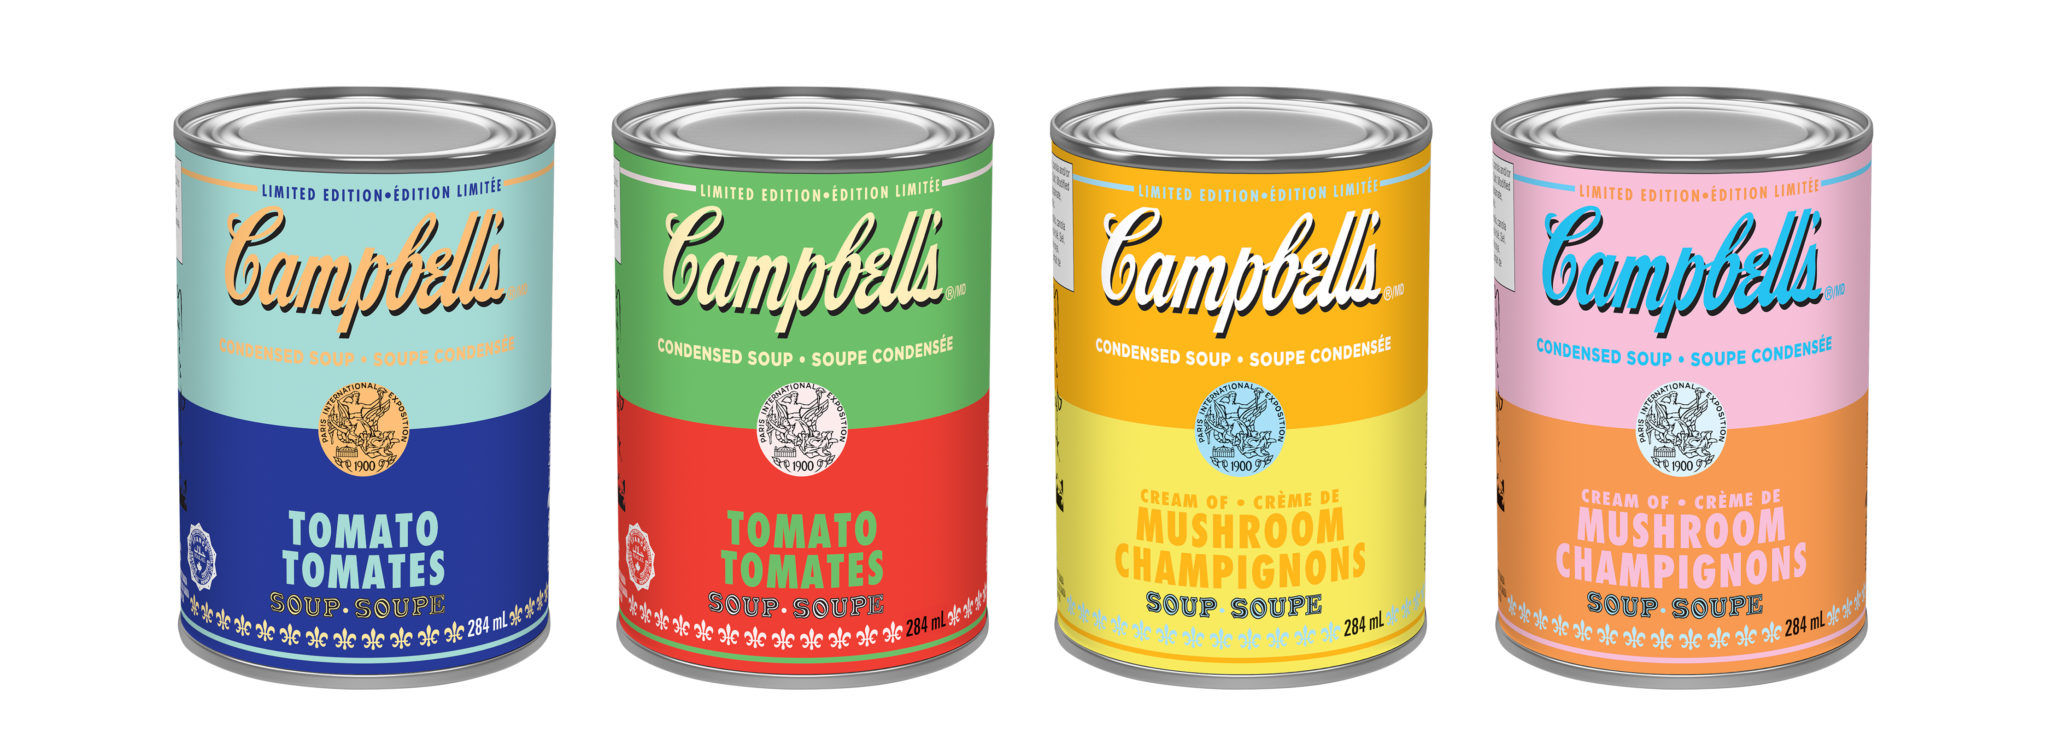
\includegraphics[width=10cm]{gfx/soupcans} \\ \medskip % Picture

\mySubtitle \\ \medskip % Thesis subtitle
%\myDegree \\
\myDepartment \\
\myFaculty \\
\myUni \\ \bigskip

\myTime\ -- \myVersion % Time and version

\vfill

\end{center}
\end{addmargin}

\end{titlepage} % Main title page

%% Back of the title page

\thispagestyle{empty}

\hfill

\vfill

\noindent\myName: \textit{\myTitle,} \mySubtitle, %\myDegree, 
\textcopyright\ \myTime

% You may wish to do something with the back of the title page, such as including your supervisors, location or time frame of the work. Below is an example of doing so although you may want to tweak it to your liking.

%\bigskip

%\noindent\spacedlowsmallcaps{Supervisors}: \\
%\myProf \\
%\myOtherProf \\ 
%\mySupervisor

%\medskip \\

%\noindent\spacedlowsmallcaps{Location}: \\
%\myLocation

%\medskip \\

%\noindent\spacedlowsmallcaps{Time Frame}: \\
%\myTime
 % Back of the title page

%\cleardoublepage% Dedication

\thispagestyle{empty}
\refstepcounter{dummy}

\pdfbookmark[1]{Dedication}{Dedication} % Bookmark name visible in a PDF viewer

\vspace*{3cm}

\begin{center}
\emph{Ohana} means family. \\
Family means nobody gets left behind, or forgotten. \\ \medskip
--- Lilo \& Stitch    
\end{center}

\medskip

\begin{center}
Dedicated to the loving memory of Rudolf Miede. \\ \smallskip
1939\,--\,2005
\end{center} % Dedication page

%\cleardoublepage\include{FrontBackMatter/Foreword} % Uncomment and create a Foreword.tex to include a foreword

%\cleardoublepage% Abstract

%\renewcommand{\abstractname}{Abstract} % Uncomment to change the name of the abstract

\pdfbookmark[1]{Abstract}{Abstract} % Bookmark name visible in a PDF viewer

\begingroup
\let\clearpage\relax
\let\cleardoublepage\relax
\let\cleardoublepage\relax

\chapter*{Abstract}
Short summary of the contents\dots a great guide by 
Kent Beck how to write good abstracts can be found here:  
\begin{center}
\url{https://plg.uwaterloo.ca/~migod/research/beckOOPSLA.html}
\end{center}

\endgroup			

\vfill % Abstract page

%\cleardoublepage% Publications - a page listing research articles written using content in the thesis

\pdfbookmark[1]{Publications}{Publications} % Bookmark name visible in a PDF viewer

\chapter*{Publications} % Publications page text

Some ideas and figures have appeared previously in the following publications:\\

\noindent Put your publications from the thesis here. The packages \texttt{multibib} or \texttt{bibtopic} etc. can be used to handle multiple different bibliographies in your document.

%\begin{refsection}[ownpubs]
%    \small
%    \nocite{*} % is local to to the enclosing refsection
%    \printbibliography[heading=none]
%\end{refsection}

%\emph{Attention}: This requires a separate run of \texttt{bibtex} for your \texttt{refsection}, \eg, \texttt{ClassicThesis1-blx} for this file. You might also use \texttt{biber} as the backend for \texttt{biblatex}. See also \url{http://tex.stackexchange.com/questions/128196/problem-with-refsection}. % Publications from the thesis page

%\cleardoublepage\usepackage{natbib}% Acknowledgements

\pdfbookmark[1]{Acknowledgements}{Acknowledgements} % Bookmark name visible in a PDF viewer

\begin{flushright}{\slshape
We have seen that computer programming is an art, \\
because it applies accumulated knowledge to the world, \\
because it requires skill and ingenuity, and especially \\
because it produces objects of beauty.} \\ \medskip
--- \defcitealias{knuth:1974}{Donald E. Knuth}\citetalias{knuth:1974} \citep{knuth:1974}
\end{flushright}

\bigskip

%----------------------------------------------------------------------------------------

\begingroup

\let\clearpage\relax
\let\cleardoublepage\relax
\let\cleardoublepage\relax

\chapter*{Acknowledgements}

\noindent Put your acknowledgements here.\\

\noindent Many thanks to everybody who already sent me a postcard!\\

\noindent Regarding the typography and other help, many thanks go to Marco Kuhlmann, Philipp Lehman, Lothar Schlesier, Jim Young, Lorenzo Pantieri and Enrico Gregorio\footnote{Members of GuIT (Gruppo Italiano Utilizzatori di \TeX\ e \LaTeX )}, J\"org Sommer, Joachim K\"ostler, Daniel Gottschlag, Denis Aydin, Paride Legovini, Steffen Prochnow, Nicolas Repp, Hinrich Harms, Roland Winkler, and the whole \LaTeX-community for support, ideas and some great software.

\bigskip

\noindent\emph{Regarding \mLyX}: The \mLyX\ port was initially done by
\emph{Nicholas Mariette} in March 2009 and continued by
\emph{Ivo Pletikosi\'c} in 2011. Thank you very much for your work and the contributions to the original style.

\endgroup
 % Acknowledgements page

    \pagestyle{scrheadings} % Show chapter titles as headings

%    \cleardoublepage% Table of Contents - List of Tables/Figures/Listings and Acronyms

\refstepcounter{dummy}

\pdfbookmark[1]{\contentsname}{tableofcontents} % Bookmark name visible in a PDF viewer

\setcounter{tocdepth}{2} % Depth of sections to include in the table of contents - currently up to subsections

\setcounter{secnumdepth}{3} % Depth of sections to number in the text itself - currently up to subsubsections

\manualmark
\markboth{\spacedlowsmallcaps{\contentsname}}{\spacedlowsmallcaps{\contentsname}}
\tableofcontents
\automark[section]{chapter}
\renewcommand{\chaptermark}[1]{\markboth{\spacedlowsmallcaps{#1}}{\spacedlowsmallcaps{#1}}}
\renewcommand{\sectionmark}[1]{\markright{\thesection\enspace\spacedlowsmallcaps{#1}}}

\clearpage

\begingroup
\let\clearpage\relax
\let\cleardoublepage\relax
\let\cleardoublepage\relax

%----------------------------------------------------------------------------------------
%	List of Figures
%----------------------------------------------------------------------------------------

\refstepcounter{dummy}
%\addcontentsline{toc}{chapter}{\listfigurename} % Uncomment if you would like the list of figures to appear in the table of contents
\pdfbookmark[1]{\listfigurename}{lof} % Bookmark name visible in a PDF viewer

\listoffigures

\vspace{8ex}
\newpage

%----------------------------------------------------------------------------------------
%	List of Tables
%----------------------------------------------------------------------------------------

%\refstepcounter{dummy}
%%\addcontentsline{toc}{chapter}{\listtablename} % Uncomment if you would like the list of tables to appear in the table of contents
%\pdfbookmark[1]{\listtablename}{lot} % Bookmark name visible in a PDF viewer
%
%\listoftables
%
%\vspace{8ex}
%\newpage
%
%%----------------------------------------------------------------------------------------
%	List of Listings
%----------------------------------------------------------------------------------------

\refstepcounter{dummy}
%\addcontentsline{toc}{chapter}{\lstlistlistingname} % Uncomment if you would like the list of listings to appear in the table of contents
\pdfbookmark[1]{\lstlistlistingname}{lol} % Bookmark name visible in a PDF viewer

\lstlistoflistings

\vspace{8ex}
\newpage

%----------------------------------------------------------------------------------------
%	Acronyms
%----------------------------------------------------------------------------------------

\refstepcounter{dummy}
%\addcontentsline{toc}{chapter}{Acronyms} % Uncomment if you would like the acronyms to appear in the table of contents
\pdfbookmark[1]{Acronyms}{acronyms} % Bookmark name visible in a PDF viewer

\markboth{\spacedlowsmallcaps{Acronyms}}{\spacedlowsmallcaps{Acronyms}}

\chapter*{Acroniemen}

\begin{acronym}[UML]
\acro{API}{Application Programming Interface}
\acro{CEO}{Chief Executive Officer}
\acro{CFO}{Chief Financial Officer}
\acro{COO}{Chief Operations Officer}
\acro{CTO}{Chief Technology Officer}
\acro{CI/CD}{Continuous Integration - Continuous Delivery/Deployment}
\acro{CVE}{Common Vulnerabilities and Exposures}
\acro{CSRC}{Computer Security Research Center (onderdeel van NIST)}
\acro{NIST}{National Institute of Standards and Technology}
\acro{OSS}{Open Source Software}
\acro{OTAP}{Ontwikkeling Test Acceptatie Productie}
\acro{SOUP}{Software of Unkown Pedigree / Provenance}
\acro{MT}{Management team}
\acro{MoSCoW}{Must, Should, Could, Won't Have (zie begrippenlijst voor uitleg)}
\acro{UML}{Unified Modeling Language}
\end{acronym}

\endgroup
 % Contents, list of figures/tables/listings and acronyms

    \cleardoublepage

    \pagenumbering{arabic} % Arabic page numbering for thesis content (1, 2, 3, etc)
%\setcounter{page}{90} % Uncomment to manually start the page counter at an arbitrary value (for example if you wish to count the pre-content pages in the page count)

    \cleardoublepage % Avoids problems with pdfbookmark

%----------------------------------------------------------------------------------------
%	THESIS CONTENT - CHAPTERS
%----------------------------------------------------------------------------------------

% Text on the Part 1 page describing  the content in Part 1
%Todo: Inleiding en Leeswijzer schrijven
%    \chapter*{Inleiding} \label{ch:inleiding} % For referencing the chapter elsewhere, use \autoref{ch:introduction}
\lipsum[01]
%Het document dat voor u ligt is een resultaat van een onderzoek en product oplevering als afstudeeropdracht door Bas Brunink voor het bedrijf Eaglescience. Het zal het process beschrijven die ik gelopen heb om een module te schrijven die automatisch een SOUP-analyse doet op zowel bestaande als nieuwe projecten.

\section{leeswijzer} \label{sec:leeswijzer}




    %Opdracht en vooronderzoek
%    \ctparttext{}
%    \part{Opdracht (Briefing)}\label{prt:opdracht}
%    % Chapter 1
\chapter{Eaglescience}\label{ch:Eaglescience} % Chapter title

Het hier beschreven onderzoek en de daarbij behorende applicatie is uitgevoerd en ontwikkeld in opdracht van het bedrijf Eaglescience. Dit bedrijf is gevestigd in Amsterdam Sloterdijk en houdt zich sinds 2009 bezig met het ontwikkelen van software. Hoewel het ontwikkelen van maatwerk software de kern activiteit is biedt het bedrijf ook een aantal andere diensten aan, zoals het bouwen van prototypes of het meedenken in een designsprint om bedrijven of startups een goede richting te geven voor het ontwikkelen van een project. Daarnaast biedt Eaglescience hosting aan voor de software die zelf is ontwikkeld, om zo garantie te kunnen bieden dat er alles aan wordt gedaan zodat de geleverde software veilig, kwalitatief goed en correct functioneerd.

\section{Organisatie}\label{sec:organisatie}
Eaglescience BV bestaat uit drie divisies: Innovations, Software en Solutions (figuur~\ref{fig:Eaglescience organogram}). Er werken, op het moment van schrijven, $\pm$ 20 medewerkers waarvan 75\% verantwoordelijk is voor de ontwikkeling van software. De andere 25\% bekleed een support rol zoals project manager, finance manager, quality manager, automatisering etc.

\begin{figure}[bth]
\myfloatalign
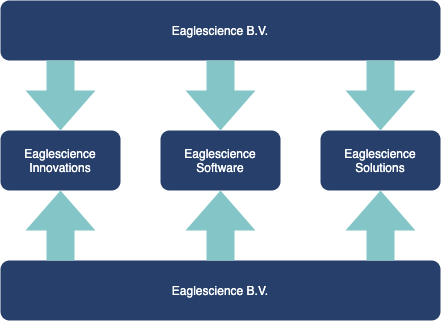
\includegraphics[width=10cm]{gfx/organogram}
\caption{Organogram Eaglescience}
\label{fig:Eaglescience organogram}
\end{figure}
De divisie Eaglescience Innovations zoekt naar nieuwe oplossingen op het gebied van softwareontwikkeling, welke door de divisie Eaglescience Software wordt geïmplementeerd. Eaglescience Solutions onderzoekt en adviseert over oplossingen voor gestelde problemen.\\

Het dagelijks bestuur is handen van:
\begin{itemize}
\item CEO / CFO - Marc Grootjen
\item CTO - Bas Breier
\item COO - Wender van Mansvelt
\end{itemize}
Onder het dagelijks bestuur valt Team Eaglescience wat bestaat uit projectmanagers en ontwikkelaars. Deze zijn onderverdeeld in diverse scrum teams die ieders verantwoordelijk zijn voor een project. De ontwikkelaars worden parallel ingezet op meerdere projecten om kennisdeling te bevorderen.

\subsection{Missie}\label{subsec:missie}

De missie van Eaglescience is het bedienen van haar partners door een ontwerp, ontwikkeling en service te bieden op het gebied van op maat gemaakte IT-oplossingen. Hiervoor heeft Eaglescience goed opgeleide IT-professionals in dienst die zichzelf continue ontwikkelen op de “cutting edge” van IT-technologie. De hoofdcompetenties van de medewerkers zijn: innovatief, intelligent, klant georiënteerd, flexibel en ambitieus.

\subsection{Visie}\label{subsec:visie}
Eaglescience streeft er als innovatief IT-bedrijf naar om software te ontwikkelen als een Business-to-Business dienst. Middels technische vaardigheden bouwen we veilige en hoogwaardige software die bijdraagt aan een betere wereld. Omdat we Agile werken, leveren we precies wat nodig is, niets meer en niets minder. Wij helpen onze klanten zoeken naar een langdurige betrokkenheid en samenwerking op basis van zowel vertrouwen als wederzijds respect.

Omdat elke vraag uniek is, ontwikkeld Eaglescience op maat gemaakte en innovatieve software.  We zijn van plan deel uit te maken van het hele proces van het formuleren van een idee tot het lanceren van het product en het waarborgen van de productie levenscyclus. Onze belangrijkste succesfactor zijn de mensen, die zich continu ontwikkelen door met de nieuwste technieken te werken op diverse projecten. Wij streven naar een optimale balans tussen werk en privé. Dit geeft onze medewerkers veel vrijheid, maar vereist zelfdiscipline en verantwoordelijkheid.

\subsection{Strategie}\label{subsec:strategie}
Eaglescience levert de visie via vier strategische thema's:
\begin{itemize}
    \item Maatschappelijke verantwoordelijkheid
    \item Persoonlijke groei en werknemer tevredenheid
    \item Kwalitatief hoogstaande producten en diensten
    \item Financieel onafhankelijk en een sociaal verantwoorde groei
\end{itemize}
We streven ernaar om veilige en hoogwaardige software diensten te leveren die waarde toevoegen aan onze samenleving. We streven naar een bedrijfscultuur waarin alle collega's hun talenten kunnen laten groeien. We hebben een ongecompliceerd werkethos: we richten ons op resultaten van hoge kwaliteit, maar met een gezonde balans tussen werk en privé en voldoende tijd voor leuke en sociale evenementen. Eaglescience verwacht van alle medewerkers dat zij hun handelen baseren op vier kwaliteitsprincipes:
\begin{itemize}
    \item Meld situaties die niet voldoen aan onze interne procedures
    \item Evalueer risico's wanneer grote veranderingen worden verwacht
    \item Help en daag elkaar uit
    \item Kennis behouden over compliancy en kwaliteitsmanagement
\end{itemize}

\section{Werkwijze}\label{sec:werkwijze}
Zoals eerder gemeld werkt Eaglescience op projectbasis met ontwikkelaars in meerdere teams. Er wordt geprobeert "full scrum" te werken waarbij de requirements van de klant centraal staan. Als een project wordt aangenomen door het managementteam dan wordt deze in sprints in samenspraak met de klant ontwikkeld. De klant wordt nauw betrokken bij het verloop van de ontwikkeling door het geven van demo's aan het einde van iedere sprint. Hier wordt gemeten hoe de applicatie zich gedraagt met betrekking tot de requirements van de klant. Dit is ook het moment dat er feedback gegeven wordt en waar nodig gestuurd kan worden in het verdere verloop. Op het moment dat er een applicatie klaar is wordt de software al dan niet overgedragen aan de klant of doorgegeven aan support en hosting die verantwoordelijk zijn voor de daadwerkelijke hosting van de software. (figuur~\ref{fig:Project Process})

%TODO: Vertaling checken
\begin{figure}[bth]
\myfloatalign
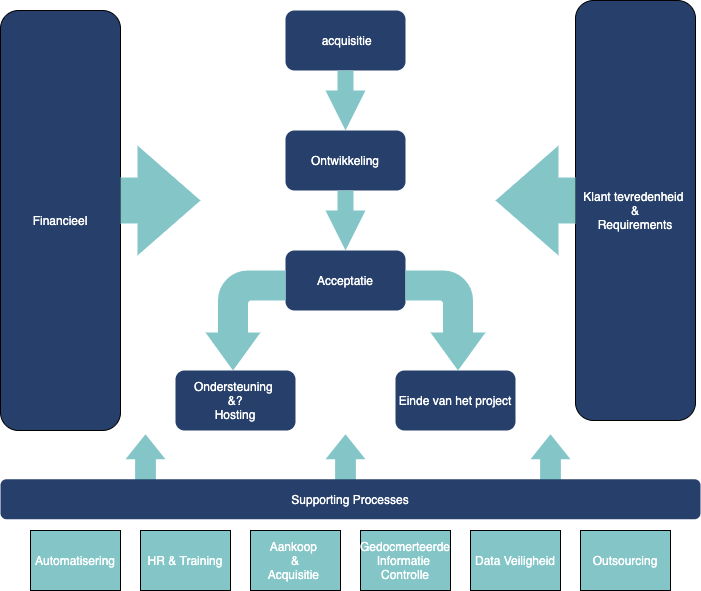
\includegraphics[width=10cm]{gfx/ProcessFlow}
\caption{Project Process}
\label{fig:Project Process}
\end{figure}

Naast het ontwikkelproces zijn er een aantal supporting processen die ervoor zorg dragen dat het bedrijf blijft draaien. Onder deze processen valt ook automatisering die voor ondersteuning zorgt van platformen waarop ontwikkeld en/of gehosted wordt. Eaglescience ontwikkeld en genereerd inkomsten op projectbasis. Alle processen die draaien moeten dus direct ingezet kunnen worden op projecten van klanten. Als er een project voor in huis gebruik wordt ondernomen moet er een duidelijk beeld zijn of er op termijn winst mee te behalen valt op monetair vlak al dan niet tijdswinst of ontwikkelgemak. (figuur~\ref{fig:Project Process})

\section{Relevante en actuele ontwikkelingen binnen Eaglescience}\label{sec:relevante-en-actuele-ontwikkelingen-binnen-Eaglescience}

Eaglescience is aan het groeien, zowel in het aantal projecten waar aan gewerkt wordt als in het aantal medewerkers. Daarnaast worden de diensten die Eaglescience aanbied ook uitgebreid, en wordt het hosten van de ontwikkelde applicaties steeds vaker aangeboden. Door deze inzet ligt de verantwoordelijkheid niet alleen bij het leveren van een veilige en hoogwaardige software, maar ook bij het leveren van een veilige hosting service. Naast de groei van het bedrijf is ook de uitbreiding van diensten die aangeboden worden een reden om taken die geautomatiseerd kunnen worden dan ook te automatiseren.

Daarnaast heeft Eaglescience de afgelopen jaren een portfolio aan verschillende klantproducten opgebouwd. Deze producten worden gehost, onderhouden en er wordt service en support geboden richting gebruikers. Eaglescience is momenteel doende dit onder de noemer Software Lifecycle Management te integreren in het kwaliteitssysteem door middel van beleid en het vastleggen in werkprocessen. Het in de grip en up-to-date houden van de live softwareproducten vraagt om een gerichte-, transparante- en traceerbare aanpak ten aanzien van alle gebruikte software-onderdelen (bibliotheken/ libraries) en onderliggende afhankelijkheden (dependencies).




%    % Chapter 2

\chapter{Opdracht}\label{ch:opdracht} % Chapter title
 % For referencing the chapter elsewhere, use \autoref{ch:examples}
Tegenwoordig zijn software-bibliotheken niet meer weg te denken in het huidige software ontwikkelproces.
Bibliotheken geven ontwikkelaars de mogelijkheid code her te gebruiken in meerdere projecten, om zo efficiënter te kunnen ontwikkelen.
Dit helpt op zijn beurt om de Time-To-Market te verkorten.
Bibliotheken kunnen door bedrijven zelf geschreven worden, in het geval van EagseScience is dit archES, of worden overgenomen van andere bedrijven/instellingen.
ArchES is echter ook afhankelijk van een aantal bibliotheken die niet ontwikkeld zijn door Eaglescience.
Hierdoor kan niet worden voorkomen dat bibliotheken worden gebruikt waarvan de afkomst niet geheel kan worden herleiden.

Deze bibliotheken vallen onder de noemer "Software of Unknown Provenance / Pedigree(SOUP)".
Door het gebruik van dit soort bibliotheken kan er een aannemelijk risico ontstaan op het gebied van kwetsbaarheden.
Om inzicht te krijgen in deze kwetsbaarheden en daarmee mogelijke veiligheidsissues dient er een SOUP-analyse gedaan te worden.
Binnen Eaglescience wordt het belang hiervan onderstreept en daarom wordt er gezocht naar een efficiënte en een waar mogelijk geautomatiseerde manier voor het uitvoeren van een dergelijke analyse om zo de veiligheid van de ontwikkelde applicaties te waarborgen zonder afbreuk te doen aan kwaliteit.

\section{Opdracht vanuit Eaglescience}\label{sec:opdracht-vanuit-eaglescience}
Vanuit de CTO is de wens ontstaan om een systematisch opgebouwde methode te ontwikkelen waarbij er automatisch periodiek een SOUP-analyse gedaan wordt op bestaande en nieuwe projecten.
Het uiteindelijke resultaat moet zijn dat er een module wordt toegevoegd aan de al bestaande portal van Eaglescience waarbij project verantwoordelijken inzicht kunnen verkrijgen in de kwetsbaarheden die in een project aanwezig kunnen zijn door het gebruik van externe bibliotheken.
%------------------------------------------------

\subsection{Eisen aan de opdracht}\label{subsec: eisen-aan-de-opdracht}

Vanuit Eaglescience zijn er een aantal eisen gesteld waaraan het eindproduct moet voldoen.
Als er aan deze eisen is voldaan is er voor Eaglescience een waardevol product welke gebruik kan worden genomen.
Daarnaast zijn er een aantal oplevereisen die gehaald dienen te worden om de kwaliteit te waarborgen.

\textbf{Functionele eisen}
\begin{itemize}
\item De module dient eenvoudig te kunnen worden gebruikt in de huidige Continuous Integration /Continuous Deployment (CI/CD) pipeline voor bestaande en nieuwe projecten
\item De module dient gebruik te maken van de bestaande huidige projectstructuur van het portal
\item De module dient ondersteuning te bieden voor meerdere omgevingen (OTAP)
\item De module dient met een instelbaar interval de analyse uit te voeren
\item De module moet op project en omgevings niveau te rapporteren over bekende kwetsbaarheden
\item De module dient kwetsbaarheden op minimaal drie niveau’s in te schalen (kritisch, gemiddeld en laag)
\item De module dient ondersteuning te bieden voor het instellen van quality gates ten aanzien melding die het vind van ieder niveau, per project, per omgeving.
\item De module wordt ontwikkeld in Angular en Play (scala), overeenkomstig bestaande portal modules
\end{itemize}
\textbf{Kwaliteitseisen}
\begin{itemize}
\item De module dient te voldoen aan de geldende kwaliteitsnormen binnen Eaglescience, minimaal meetbaar door:
	\begin{itemize}
	\item test coverage > 70\%
	\item onderdeel van de bestaande CI/CD voor het Eaglescience Portal
	\end{itemize}
\item De geschreven code dient gereviewd te worden door een Eaglescience ontwikkelaar
\item In de module dient gescheiden componenten te beavtten: Frontend, Backend, API
\item De module dient goed gedocumenteerd te zijn.
\item Voor de API dient gebruik gemaakt te worden van swagger.
\end{itemize}

\subsection{Deliverables vereiste resultaten}\label{subsec:deliverables-vereiste-resultaten}
Vanuit de CTO zijn er naast de functionele eisen ook eisen gesteld aan de oplevering:
\begin{itemize}
\item Geïntregreerde en aantoonbaar werkende module
\item De code van de module gepubliceerd in Eaglsescience GitLab
\item API documentatie genereren middels swagger
\item Een handleiding hoe de module gebruikt dient te worden
\item Eventuele aanvullende deliverables vanuit de HvA
\end{itemize}



[Eerst onderzoek afmaken dan aanpassen]
\section{Opdracht fasen}\label{sec:opdracht-fasen}
Om de hierboven beschreven opdracht zo goed als mogelijk uit te voeren dient er eerst een onderzoek gedaan worden naar het begrippen binnen het domein SOUP en daarnaast naar mogelijkheden om bibliotheken te screenenen te testen op kwetsbaarheden.
Na de onderzoeksfase  moet er een module ontwikkeld worden die deze mogelijkheid implementeerd met in achtneming van de bovengenoemde eisen.

\subsection{Fase 1: Onderzoek} \label{subsec:fase-1:-onderzoek}
%[OOk onderzoek over tooling binnen Eaglescience benoemen]
Als eerste dient er een begrippen / literatuur onderzoek gedaan te worden binnen het domein SOUP om een goede kennis te vergaren over het domein om een basis te kunnen leggen voor een te implementeren module.

Daarnaast dient er onderzoek gedaan te worden om te zien of er bibliotheken en resources zijn waar informatie over SOUP-bibliotheken te vinden is, en aan welke eisen deze bivbliotheken moeten voldoen om kwetsbaar te worden.
Hier lettende op de eisen vanuit Eaglescience en de mogelijkheden die deze analyse bibliotheken bieden.
Deze fase wordt beschreven in het tweede deel van dit document.

\subsection{Fase 2: Oplevering SOUP analyse module}\label{subsec:fase-2:-oplevering-soup-analyse-module}
De uit het onderzoek behaalde resultaten ten opzicht van beschikbare resources om een SOUP-analyse te voeden moet worden geïmplementeerd in een module binnen een bestaande applicatie.
Deze module moet voldoen aan de eisen die gesteld zijn.
Het ontwerp en implementatie wordt beschreven

\section{plan van aanpak}\label{sec:plan-van-aanpak}
Het plan is als volgt:
\begin{enumerate}
	\item LiteratuurOnderzoek
	\item Markt onderzoek
	\item Resultaat onderzoek
	\item ontwerp implementatie
	\item Ontwikkeling implementatie
	\item Deploy implementatie
\end{enumerate}




\section{mindmap test}\label{sec:mindmap-test}
Kijken of dit nog waardevol is:

\begin{tikzpicture}[grow cyclic, text width=2.7cm, align=flush center,
	level 1/.style={level distance=5cm,sibling angle=90},
	level 2/.style={level distance=3cm,sibling angle=45}]

\node{ShareLaTeX Tutorial Videos}
child { node {Beginners Series}
	child { node {First Document}}
	child { node {Sections and Paragraphs}}
	child { node {Mathematics}}
	child { node {Images}}
	child { node {bibliography}}
	child { node {Tables and Matrices}}
	child { node {Longer Documents}}
}
child { node {Thesis Series}
	child { node {Basic Structure}}
	child { node {Page Layout}}
	child { node {Figures, Subfigures and Tables}}
	child { node {Biblatex}}
	child { node {Title Page}}
}
child { node {Beamer Series}
	child { node {Getting Started}}
	child { node {Text, Pictures and Tables}}
	child { node {Blocks, Code and Hyperlinks}}
	child { node {Overlay Specifications}}
	child { node {Themes and Handouts}}
}
child { node {TikZ Series}
	child { node {Basic Drawing}}
	child { node {Geogebra}}
	child { node {Flow Charts}}
	child { node {Circuit Diagrams}}
	child { node {Mind Maps}}
};
\end{tikzpicture}

%    \chapter{Conclussie}\label{ch:opdrachtconclussie}

De opdrachtgever is EagleScience, welke als opdracht "zoek een methode om geautomatiseerd en periodiek een SOUP analyse te doen op kwetsbaarheden" EagleScience wil dit graag ontwikkelen omdat men een groei in zowel projecten als personeel ziet aankomen. Daarnaast is er een proces gaande om de Software Lifecycle Management welke nu in de praktijk al wordt uitgevoerd in een beleid te gieten. Het is in deze context goed om te meten welke kwetsbaarheden er zijn binnen een ontwikkelde applicatie. Echter is het voorkomen beter. Door het gebruik van deze module komt er inzicht in deze kwetsbaarheden en wordt als het goed is  de vraag opgeworpen of het gebruik van deze bibliotheek nog wel gerechtvaardigd is.




    % onderzoek
    \ctparttext{}
    \part{Onderzoek}\label{prt:Onderzoek}
%    % Chapter 3

\chapter{Inleiding}\label{ch:inleiding3} % Chapter title


\label{inOnderzoek} % For referencing the chapter elsewhere, use \autoref{ch:InOnderzoek}

[NOTE: ]Verplaatst naar hethoofdstuk Onderzoeksmethode



\section{Scope}\label{sec:scope}
[NOTE: ]verplaatst naar het hoofdstuk Onderzoeksmethode

De volgende onderwerpen worden in deze hoofdstukken beschreven:
\begin{itemize}
    \item Onderzoeksmethode, een beschrijving van de gebruikte methoden en aanpak van de beide onderzoeken.
    \item Onderzoek: Architectuur binnen eaglescience, een onderzoek naar de gebruikte architectuur binnen Eaglescience als ook de werkwijze waarop Eaglescience software ontwikkeld.
    \item Onderzoek: SOUP-analyse, een onderzoek over wat SOUP precies is welke gevaren er potentieel mee gemoeid gaan, en welke oplossingen er bestaan om SOUP-analyses te doen.
\end{itemize}

    \chapter{Onderzoeksplan}\label{ch:onderzoekPlan}

In het vorige hoofdstuk is de opdracht voor dit onderzoek duidelijk uitgeschreven. In dit hoofdstuk wordt uitgewijd over hoe deze opdracht wordt uitgevoerd, welke bronnen er gebruikt worden en hoe het onderzoek gedaan zal worden. Het resultaat is het een onderzoeksplan voor een onderzoek naar analyses op kwetsbaarheden op externe bibliotheken(SOUP) binnen EagleScience. Als leidraad voor dit hoofdstuk is gekozen voor hoofdstuk 4 uit \cite{JanLeen2017}

\section{Aanleiding}\label{sec:OP_aanleiding}
EagleScience heeft de ambitie om te groeien in zowel het aantal projecten dat het aanneemt als in het aantal medewerkers. Daarnaast is het bezig met het integreren van het software lifecycle management paradigma in het kwaliteitssysteem om zo een gerichte-, transparante en traceerbare aanpak te hebben over de kwaliteit en daarmee de veiligheid van de te leveren software. Vooral de groei in projecten heeft geleid tot deze opdracht. Het feit dat EagleScience aanbied om de door ons ontwikkelde applicaties te hosten voor de klant zullen deze in de komende tijd ook aannemen. Hierdoor neemt de druk op het DevOps team binnen EagleScience toe. Om deze druk te verminderen wordt er gezocht naar manieren om taken die veel voorkomen en bijdragen aan de kwaliteit te automatiseren om op die manier een traceerbare en transparante aanpak te hebben.

\section{Probleemanalyse}\label{sec:probleemanalyse}
[NOTE: WIE< WAT< WAAR< WAAROM< WANNEER< WAARDOOR]
EagleScience doet veel om veilige applicaties te leveren voor haar klanten. Tijdens het ontwikkelproces wordt er door de ontwikkelaars continue afgewogen welke maatregelen, in architectuur en/of code, moeten worden genomen applicaties veilig op te leveren. Deze afwegingen zijn onderdeel van het ontwerpproces en worden door de klant gezien als declarabele uren en zijn ook bereid voor deze werkzaamheden te betalen. Op het moment dat een project "klaar" is over gaat van ontwikkeling naar hosting. Wordt er onderhoud gedaan volgens afspraken in de SLA. In diezelfde SLA wordt niet altijd ruimte opgenomen voor het analyseren van de applicatie op kwetsbaarheden. Vaak komt dit doordat de klant er geen budget voor heeft, of het niet belangrijk vindt. Gezien EagleScience alleen een advies kan uitbrengen over support en de klant de eindbeslissing heeft. Maar omdat EagleScience wel zo "veel mogelijk" wil garanderen dat de software die gehost wordt veilig is dient de applicatie in hosting periodiek geannalyseerd worden op kwetsbaarhebeb. Op dit moment is dit een tijdrovend handmatig process waarbij een teamlid ongeveer 8 tot 12 bezig om iedere dependency te bekijken of er updates zijn en welke mogelijke kwetsbaarhden er zijn. Door de groei die EagleScience binnenkort wil maken is er de wens om bovestaand proces te automatiseren.

Er moet dus een methode worden ontwikkeld die het mogelijk maakt om geautomatiseerd en periodiek een analyse te doen op dependencies die gedeclareerd zijn in het project. De analyses moeten inzichtelijk maken welke componenten er genanalyseerd zijn inclusief versie nummer. En of er kwetsbaarheden zijn gevonden in deze bibliotheken. De methode moet voor alle platformen(Docker, Programmeertalen, Databases etc.) dezelfde resultaten geven.

Door de analyses te automatiseren wordt beoogd dat er minder tijd wordt besteed aan de analyse. Deze tijd kan dan worden besteed door de ontwikkelaar aan taken die declarabel zijn en voor beide partijen winstgevend zijn.


%Probleem stelling
Samengevat is het probleem als volgt: "Handmatig SOUP-analyses doen kost tijd die niet declarabel zijn. Om deze reden is de wens dat er een geautomatiseerde oplossing komt die periodiek de projecten die in ontwikkeling zijn en/of gehost worden door EagleScience geanalyseerd wordt op kwetsbaarheden in gebruikte externe bibliotheken. Door deze automatische oplossing wordt ingeschat dat de (niet declarabele) uren die normaal gebruikt worden voor analyseren van de projecten gebruikt kunnen worden voor andere wel declarabale uren.

De huidige handmatig uitgevoerde SOUP-analyses zijn tijdrovend waardoor ontwikkelaars andere taken moeten laten vallen. Daarnaast wordt de analyse niet frequent genoeg gedaan en vaak enkel op inplanbare momenten. De probleemstelling luidt: "Ontwikkel een methode die automatisch en periodiek een SOUP-analyse doet op de projecten die EagleScience in haar beheer heeft".

Centrale vraagstelling:





\section{Doelstellingen}\label{sec:doelstellingen}
Het doel van dit onderzoek is het ontwikkelen van een methode om een SOUP-analyse te doen binnen de dev-stack van EagleScience. Hierbij moet rekening gehouden worden met de in de opdracht gegeven criteria, waarvan de belangrijkste is dat er zo min mogelijk impact moet zijn op de huidige werkwijze. Aan het einde van het onderzoek moet dus een methode worden gepresenteerd die vervolgens bewezen kan worden middels een implementantie van een  analyse op de twee meest gebruikte technologiën binnen EagleScience. De implementatie wordt dan ook in deel \ref{prt:Implementatie} beschreven.


\section{Stakeholdersanalyse}\label{sec:stakeholdersanalyse}
Om te kijken naar het draagvlak voor dit onderzoek dient er een stakeholders analyse gedaan te worden. Op deze manier moet het duidelijk worden wie de stakeholders zijn en welke belangen zei hebben bij het doen van een onderzoek naar een geautomatiseerde SOUP-Analyse en de resultaten hiervan.

\subsection{Dagelijks bestuur (intern)}\label{subsec:dagelijks-bestuur-(intern)1}
Het dagelijks bestuur ziet vooral voordelen in het op een overzichtelijke manier verkrijgen van inzichten in kwetsbaarheden. Zij beogen dat ze hierdoor beter kunnen aansturen in het gebruik van bibliotheken en/of andere technologiëen. Ondanks dat de ontwikkeling van de beoogde nieuwe module vooral geld zal kosten, is de huidige manier van werken ook niet kosten-effectief. Daarnaast voorziet de CTO dat de nieuwe module tijdswinst zal opleveren waardoor de time-to-market voor andere projecten hoger kan komen te liggen en er dus op langer termijn meer verdiend kan worden.

\subsection{Projectmanagers (intern)}\label{subsec:projectmanagers-(intern)1}
Project managers krijgen op dit moment een update over de staat van kwetsbaarheden op het moment dat een analyse gedaan is. Veelal na een deploy of als er naar gevraagt is. De nieuwe module zal ze echter de mogelijkheid bieden om up-to-date informatie on-demand te verkrijgen.
De tijdsinvestering die nodig is van ontwikkelaars voor de ontwikkeling van de module weegt volgens hen op tegen de voordelen die de module in de toekomst kan brengen.

\subsection{Ontwikkelteam (intern)}\label{subsec:ontwikkelteam-(intern)1}
Het handmatig testen van kwetsbaarheden werd tot op heden gedaan door het ontwikkelteam. Dit is een tijdrovende taak, welke ten koste gaat aan de ontwikkeling van software voor klanten. Het ontwikkelteam heeft daarrom direct baat bij de ontwikkeling van de beoogte module en wil daarom graag hieraan meedenken en meewerken.

\subsection{Klant (extern)}\label{subsec:klant-(extern)1}
De enige externe stakeholder is de klant. Dit is tevens een passieve stakeholder gezien zij niet direct betrokken zijn bij de ontwikkeling van de module, maar wel baat hebben bij de uitkomst hiervan, namelijk in de vorm van veiligere en betrouwbaardere software tegen potentieel lagere kosten.

\subsection{Stakeholder analyse}\label{subsec:stakeholder-analyse1}
\begin{figure}[H]
    \myfloatalign
    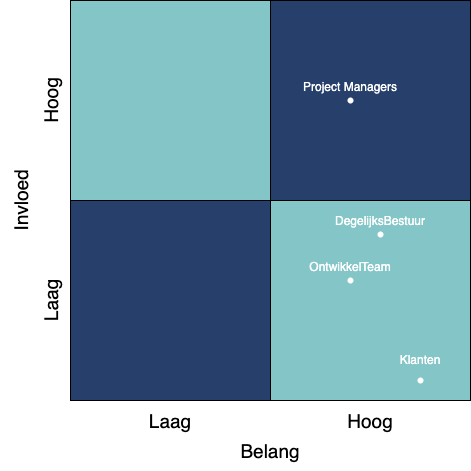
\includegraphics[width=10cm]{gfx/stakeholderanalyse}
    \caption{StakeHolders Analyse}
    \label{fig:StakeholderAnalyse1}
\end{figure}
[NOTE]Figuur stakeholder analyse nog aanpassen.
Zoals te zien is in figuur~\ref{fig:StakeholderAnalyse1} zijn de projectmanager, het ontwikkelteam en de klanten het meest gebaad bij een nieuwe module voor de analyse van kwetsbaarheden.
Door deze analyse worden alleen de requirements meegenomen die intern zijn opgenomen.


\section{Theoretisch kader}\label{sec:theoretisch-kader}

Het theoretisch kader waarmee gewerkt wordt bestaat uit twee hoofddelen. Het eerste hoofddeel is de werkwijze van EagleScience en de gebruikte technologiëen. De volgende bronnen zullen bij het onderzoek worden gebruikt:
\begin{itemize}
    \item \textbf{151030 F04B Proces Flow Chart ES\_V1.0\_TN.pdf} een document dat de workflow beschrijft die binnen EagleScience gehanteerd wordt.
    \item \textbf{200121\_Policy Manual\_ES\_V6 signed.pdf} ISO handboek waarin de bedrijfsvoering binnen EagleScience wordt beschreven.
\end{itemize}
Deze documenten vormen de basis over de werkwijze van EagleScience en zal als input gelden voor het ontwerp dat plaats gaat vinden na het onderzoek.

Het tweede hoofddeel is de theorie over externe bibliotheken. Het richt zich op het gebruik hiervan, de potentiële gevaren en methoden om deze bibliotheken te analyseren. Als ingangspunt is de OWASP Top-10 gekozen omdat de inhoud van dit document binnen EagleScience geldt als aandachtspunten voor het ontwikkelen van veilige software. De basis voor dit onderzoek wordt beschreven in punt "A06:2021-Vulnerable and Outdated Components". Hier wordt beschreven welke gevaren er potentieel dreigen als op dit punt niets gedaan wordt. Andere bronnen zijn:
\begin{itemize}
    \item \textbf{OWASP top 10 (https://owasp.org/Top10/)} hierin staan de belangrijkste aandachtspunten die door een onderzoek vanuit de OWASP aan het licht zijn gekomen. Op A06:2021 staat een melding over kwetsbaarheden en outdated Components.
    \item \textbf{Detail pagina OWASP A06:2021(https://owasp.org/Top10/A06_2021-Vulnerable_and_Outdated_Components/)} OP deze pagina zijn details te vinden over item A06:2021 waaronder een beschrijving, Hoe het te voorkomen is en een aantal voorbeeld scenario's waarbij een aanval wordt geillustreerd.
    \item \textbf{OWASP dependency-check (https://owasp.org/www-project-dependency-check/)} Pagina over het project binnen de OWASP voor het analyseren van componenten in Applicaties
    \item \textbf{Justifying the use of software of uncertain pedigree (SOUP) in safety-related applications} P.G.\ Bishop, R.E.\ Bloomfield and P.K.D.\  Froome for Adelard 2001. Hoewel dit document verouderd lijkt staat er wel degelijk interessante informatie over waarom je SOUP zou gebruiken en hoe je de risico's kan verminderen.
    \item \textbf{Backstabber’s Knife Collection: A Review of Open Source Software Supply Chain Attacks} Marc Ohm, Henrik Plate, Arnold Sykosch, and Michael Meier: 2020: Dit artikel bevat informatie over een mogelijke vorm van aanvallen die middels SOUP uitgevoerd zouden kunnen worden. Daarnaast geeft het artikel inzicht in hoe de onderzoekers packages voor NPM, Python, en Ruby hebben onderzocht.
\end{itemize}
Het laatste hoofddeel bestaat uit de resultaten van de bovengenoemde onderdelen waarmee een voor EagleScience geschikte methode wordt gevonden. Naast de resultaten van de twee voorgaande hoofddelen worden de volgende bronnen geraadpleegd als leidraad voor het ontwerp:

\section{Conceptueel model}\label{sec:conceptueel-model}
Om de relevantie en relatie van de verschillende onderzoeken te waarborgen is het volgende conceptueel model opgesteld.
\begin{figure}[H]
    \centering
    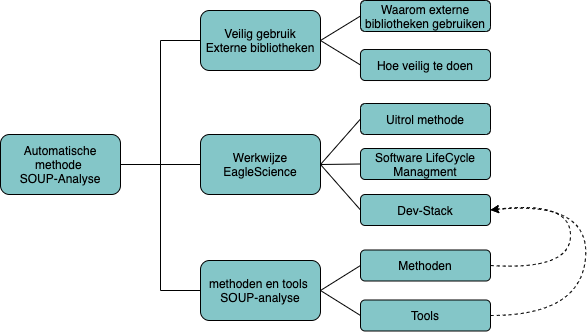
\includegraphics[width=12cm]{gfx/Conceptueel Model}
    \caption{Conceptueel Model}
    \label{fig:ConceptueelModel}
\end{figure}

In figuur~\ref{fig:ConceptueelModel} is het conceptueel model opgenomen dat voor deze opdracht is opgesteld. Dit model maakt de samenhang van de verschillende begrippen duidelijk.

Het kernbegrip is "Automatische methode SOUP analyse" en staat voor de eind conclusie die het onderzoek moet opleveren in de zin van een conclussie over tools en een methode die gebruikt kunnen worden in het ontwerp van de module. Om tot deze conclussie te komen zijn er vier begrippen die ieders een eigen domein binnen de probleemstelling belichten. Zo zal "werkwijze EagleScience" de manier van werken binnen Eaglescience belichten als ook de manier van uitrollen en de dev-stack die gebruikt gaat worden. Ook komt hier de Software Lifecycle Managment aan bod gezien dit één van de aanleidingen voor de opdracht. Het theoretische deel van het onderzoek wordt onderzocht in "veilig gebruik externe bibliotheken" waarin wordt gekeken waarom er bibliotheken van buitenaf worden gebruikt en wat de potentiële gevaren zijn die dit met zich meebrengt. Het begrip methoden en tools zal ingaan op de beschikbare tools die gebruikt kunnen worden om een analyse te doen. Met deze tools wordt een methode onderzocht die het mogelijk maakt met de constraints die EagleScience heeft om een SOUP analyse te doen. Met als resultaaat een theoretische methode die als input kan gelden voor het ontwerp voor de nieuwe module die in de opdracht staat beschreven. Deze nieuwe module dient in de EagleScience Portal opgenomen te worden en om die reden is het begrip "Huidig architctuur EagleScience Portal" waarin wordt onderzocht hoe de portal ontworpen is en welke dev-stack er is gebruikt.

\section{Deelvragen}\label{sec:deelvragen}
Aan de hand van het theoretisch kader, conceptueel model en de doelstellingen zijn er de volgende deelvragen voor dit onderzoek opgesteld:
\textbf{Dev-stack binnen Eaglescience}
\begin{itemize}
   % \item Hoe wordt binnen EagleScience het software lifecycle management paradigma ingevoerd?
    \item Welk proces wordt er binnen EagleScience gebruikt om software te ontwikkelen en hoe resulteert dit is een dagelijkse werkwijze?
    \item Wat zijn de meest gebruikte ontwikkeltalen en frameworks die binnen EagleScience worden toegepast?
    \item Welke tooling wordt er gebruikt binnen EagleScience? [NOTE relevant?]
    \item Hoe wordt er binnen EagleScience software uitgerold?
\end{itemize}
\textbf{Waarom externe biibliotheken gebruiken?}
\begin{itemize}
    \item Welke methodes en tools zijn er beschikbaar voor SOUP analyse?
\end{itemize}
\textbf{Methodes om een SOUP analyse te doen binnen de Dev-stack van EagleScience}
\begin{itemize}
    \item Welke tools bestaan er om dependency informatie uit een sbt en npm project te halen?
    \item Hoe zijn de tools in te zetten in de huidige projecten?
    \item Welke output wordt er verkregen van de tools?
    \item Welke manieren zijn er om uit de huidige pipeline informatie over de deploy te halen?
    \item Wat zijn hier de voor-, en nadelen van?
\end{itemize}


\section{Onderzoeksontwerp}\label{sec:onderzoeksontwerp}
Gezien de grote hoeveelheid deelvragen die benoemd zijn op basis van de onderzoeksvraag en het conceptueel model is het verstandig om het onderzoek in kleinere deelonderzoeken te verdelen. Door het op te delen in deelonderzoeken kan het kader beter worden vastgesteld en zal er minder snel "teveel" worden onderzocht. De deelonderzoeken zullen op de volgende manier worden opgesplitst:
\begin{enumerate}
    \item \textbf{Werkwijze en dev-stack EagleScience} Dit onderzoek moet inzicht geven in de dagelijkse manier van werken binnen EagleScience en de daarbij gebruikte dev-stack. Het doel is inzicht verkrijgen in hoe EagleScience applicaties ontwikkeld, hoe deze uitgerold worden en hoe er op dit moment SOUP analyses worden uitgevoerd.
    \item \textbf{Theorie SOUP analyses} Om een methode te kunnen ontwikkelen is er een theoretische basis nodig. Dit onderzoek geeft inzicht in de theoretische basis en het belang van SOUP analyses. Daarnaast wordt er uitgezocht hoe er het beste een analyse gedaan kan worden.
    \item \textbf{Methode voor SOUP analyse binnen EagleScience} Door inzichten uit voorgaande onderzoeken te combineren en nieuwe kennis toe te voegen is er een ontwerp voor een implementatie die aan de opdracht voldoet.
\end{enumerate}

\subsection{strategie}\label{subsec:opstrategie}
Om de drie onderzoeken die hierboven beschreven zijn goed uit te kunnen voeren zijn er de volgende strategieen bedacht die ervoor zorgen dat er een betrouwbaar resultaat is waar verder mee gewerkt kan worden.
Voor het onderzoek binnen de huidige situatie binnen EagleScience wordt interne documentatie geraadpleegd aangevuld met vraag gesprekken met collega's die met het onderwerp te maken hebben. Deze gespreken zullen worden gehouden in delen gezien de manier waarop er binnen EagleScience gewerkt wordt. (heeft te maken met het aantal niet declarabele uren die ieder persoon wel of niet heeft). Het onderzoek naar de theorie van SOUP analyses wordt uitgevoerd middels een deskresearch waarbij in literatuur gezocht wordt naar methoden om de analyse te doen. Daarnaast wordt er een selectie gemaakt in tools die al ontwikkeld zijn die bruikbaar zijn voor het einddoel van de opdracht. In het laatste onderzoek wordt gekeken naar een method die past bij de huidige manier van werken binnen eaglescience, en de tools die gevonden zijn. Ook wordt er een ontwerp gemaakt hoe de methode eruit komt te zien er welke data dit oplevert waarna er een module ontwikkeld kan worden die deze data inzichtelijk maakt voor de stakeholders.

\section{planning}\label{sec:planning}
Om tijdig tot resultaten te komen is de volgende planning opgesteld.

\subsection{Requirements analyse \textbf{september 2021}}\label{subsec:requirements-analyse}
Na het ontvangen van de opdracht dient er onderzocht te worden of er naast de eisen die door de CTO in de opdracht zijn gezet nog andere eisen zijn binnen EagleScience. Hiervoor zal er onderzocht worden welke betrokkenen er zijn en welke belangen en wensen zij hebben. Na het houden van interviews zullen alle wensen tegen elkaar worden afgewogen. Dit zal leiden tot een document waarin alle belangrijke requirements worden geprioriteerd volgens de MoSCoW\-methode.

\textbf{Methode:} Intake gesprek met opdrachtgever, interviews met betrokkenen, enquete voor ontwikkelaars.

\textbf{Resultaat:} Applicatie requirements document.

\subsection{Vooronderzoek \textbf{september 2021 - oktober 2021 }}\label{subsec:onderzoek}
Om de requirements om te kunnen zetten naar een ontwerp zal er onderzoek gedaan worden naar de huidige manier van ontwikkelen en compileren van de software. Een onderzoek naar begrippen binnen het domein SOUP is een voorwaarde om vervolgens onderzoek te kunnen doen naar methodes om analyses te kunnen doen op software die EagleScience maakt ten opzichte van SOUP. De resultaten van het vooronderzoek zullen worden gebruikt als input.
Om meer kennis en verdieping te krijgen in de materie rondom de nieuwe module zullen er een aantal onderzoeken worden uitgevoerd.


Er is onderzoek nodig naar de volgende onderwerpen:
\begin{itemize}
    \item \textbf{Architectuur binnen EagleScience} Werkwijze en ontwikkel stack van EagleScience met daarin specifiek onderzocht hoe er omgegaan wordt met het voorkomen van onveiligheden in de geleverde software
    \item \textbf{Externe bibliotheken gebruik en het gevaar} Onderzoek naar waarom er externe bibliotheken worden gebruikt en het gevaar hiervan.
    \item \textbf{Soup Analyse} Door te kijken naar de kwetsbaarheden in de externe bibliotheken kan er beter worden nagegaan of er kwetsbaarheden in de software zitten. Dit onderzoek zal in gaan op het bestaan van methodes om SOUP analyses te doen. En een mogelijkheid om dit (deels) geautomatiseerde te doen.
\end{itemize}

\textbf{Methode:} Bureau onderzoek, interviews met specialisten, meedoen aan en/of terugkijken van conferenties

\textbf{Resultaat:} Inzicht in het begrip SOUP en software veiligheid als ook een idee voor een mogelijke implementatie van de oplossing die voor EagleScience de beste is zonder veel impact op de huidige manier van werken te hebben.

\subsection{Initieel ontwerp \textbf{oktober 2021 - november 2021 }}\label{subsec:initieel-ontwerp}
Er zal een ontwerp worden gemaakt waarin vast gelegd is welke requirements er beslist in de module moeten zitten en de uitwerking van deze. Evenals een ontwerp van de architectuur en het datamodel. Naast de module zal er ook een ontwerp gemaakt worden voor een ontwikkel/test omgeving om de module continue te kunnen testen zonder dat dit de huidige buildstraat beinvloed. Dit laatste is van belang om zo min mogelijk storingen te veroorzaken in de dagelijkse gang van zaken bij al lopende projecten. Het eerste ontwerp zal als leidraad dienen voor de implementatie waarin afgeweken kan worden als dit nodig blijkt tijdens de implementatie sprints.

\textbf{Methode:} Overleggen met ontwikkelaars, huidige omgeving onderzoeken op mogelijkheden en architectuur.
\textit{wellicht nog toevoegen als resultaten: blokdiagram van oplossing/architectuur; sequence diagram om te komen van analyse tot rapportage (er is een handig tooltje om deze diagrammen te tekenen: https://bramp.github.io/js-sequence-diagrams/)}
\textbf{Resultaat:} Eerste ontwerp in de vorm van een datamodel, blokdiagram van architectuur voor de oplossing, als ook een sequence diagram om van analyse tot rapportage te komen.

\textit{4.4: Gebruik hier of de template ontwikkel omgeving voor (aparte branch/taak); of de portal ontwikkelomgeving
4.4: Voeg rij resultaat toe: klaar voor review of gereviewde}

\subsection{Implementatie en Testen \textbf{november 2021 - januari 2022 }}\label{subsec:implementatie-en-testen}
Om te kunnen beginnen aan de implementatie is er een ontwikkel/ test omgeving nodig die het mogelijk maakt om zonder invloed op de dagelijkse werkzaamheden van EagleScience een module te kunnen ontwikkelen. Deze zal eerst worden opgezet. Als test projecten zullen snapshots worden gebruikt van de daadwerkelijke projecten dit om een zo accuraat mogelijke test omgeving te hebben. Zoals in de opdracht beschreven dient de nieuwe module een onderdeel te zijn van de bestaande portal. Er zal dan ook direct samen worden gewerkt met het team die daar op het moment mee aan het ontwikkelen is. Tijdens de implementatie zal er ook worden gedocumenteerd wordt hoe de module werkt en welke procedures hier in worden gevolgd. Dit document biedt ontwikkelaars de mogelijkheid om dit door te nemen als on-boarding en referentie.

\textbf{Methode:} Agile scrum sprints met iedere 2 weken een oplevermoment en demo als ook een reflectie op de sprint.
\textbf{Resultaat:} Werkende en geteste applicatie die klaar is om uitgerold te worden.

\subsection{Uitrollen en documentatie \textbf{januari 2022 - februari 2022 }}\label{subsec:uitrollen-en-documentatie}
Nadat de implementatie van de meest kritische requirements is afgerond zal er worden begonnen met het uitrollen van de module en het testen door een geselecteerde groep gebruikers. De feedback wordt bekeken en meegenomen in de evaluatie. Mocht het nodig zijn dan zal er accuut actie worden ondernomen om deze wijzigingen aan te passen. Mochten er wensen zijn die kunnen wachten dan zal er worden overwogen om deze mee te nemen in de volgende iteratie van het project. (de verwachting is dat de module die hier beschreven wordt verder zal worden uitgebreid met de diverse mogelijkheden om betere en veiligere software te ontwikkelen.) Daarnaast zal ook de documentatie verder worden afgerond.
\textbf{Methode:} Interviews met stakeholders met een analyse over de nieuwe requirements.

\textbf{Resultaat:} Uitgerolde en gedocumenteerde applicatie

%    % Chapter 3

\chapter{Onderzoeksmethode}\label{ch:onderzoeksmethode} % Chapter title

Zoals in de inleiding vermeld zijn er twee onderzoeken benodigd om deze opdracht te kunnen volbrengen.
In de komende secties is te vinden welke methode, stategiën en scoping zijn gebruikt om een resultaat te vinden.
Waarbij iedere sectie een onderzoek vertegenwoordigd


\section{Onderzoek: Architectuur binnen Eaglescience}\label{sec:onderzoeksmethode-architectuur-binnen-eaglescience}
Het resultaat van dit onderzoek moet zijn: "Het hebben van inzicht in de manier van werken binnen Eaglescience en de daarbij horende keuzes voor ontwikkeltalen, architectuur, en tools".
Om deze inzicht te krijgen is het volgende onderzoeksmodel (figuur:\ref{fig:Onderzoeks model Eaglescience}) opgesteld waarbij er vanuit eigen kennis, interne workshops en vooronderzoek gekeken is naar gebruikte ontwikkelingstalen en tooling.
Deze is vervolgens geverifieerd met senior developers.
Hieruit is vervolgens het resultaat in de vorm van inzicht in de huidige dev-stack naar voren gekomen.
\begin{figure}[h!] %todo: Nog in kleur zetten van Eaglescience als deze goed is.
  \myfloatalign
  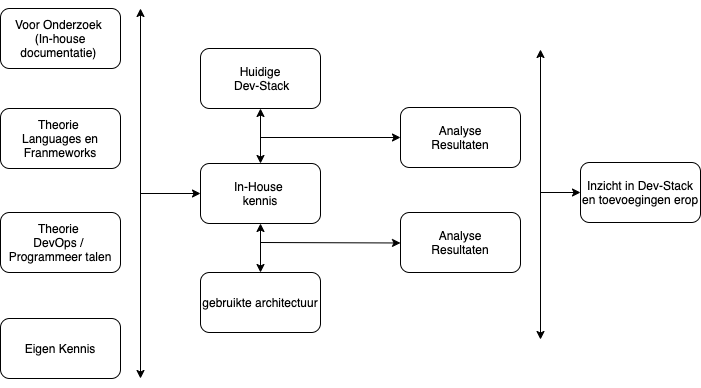
\includegraphics[width=10cm]{gfx/OnderzoeksmodelES}
  \caption{Onderzoeksmodel Eaglescience}
  \label{fig:Onderzoeks model Eaglescience}
\end{figure}

Zoals vermeld is er eerst vanuit eigen kennis, vooronderzoek en kennis opgedaan in de door Eaglescience workshops een lijst gemaakt met de gebruikte technieken.
Daarna is deze geverifieerd met senior ontwikkelaars doormiddel van interviews.
Tijdens deze interviews is ook ruimte geweest voor de reden en filosofie achter de keuzes die er gemaakt zijn in het gebruik van de talen.

\section{Onderzoek naar SOUP-analyse}\label{sec:onderzoek-naar-soup-analyse}
Dit onderzoek heeft als ingang het gegeven dat er kwetsbaarheden in de bibliotheken zitten met daarbij de dev-stack van Eaglescience.
Het resultaat van dit onderzoek moet zijn dat er een methode moet zijn waarbij er een assesment op de bestaande dev-stack binnen de werkwijze van Eaglescience moet komen die geimplementeerd kan worden.
Het onderzoekmodel (figuur:\ref{fig:Onderzoeks model Dev-Stack}) geeft weer dat de ingangs kennis de opgedane kennis uit het onderzoek naar de architectuur van Eaglescience en een literatuur studie naar mogelijkheden om soup te analyseren.

\begin{figure}[h!] %Todo: Nog in kleur zetten van Eaglescience als deze goed is.
  \myfloatalign
  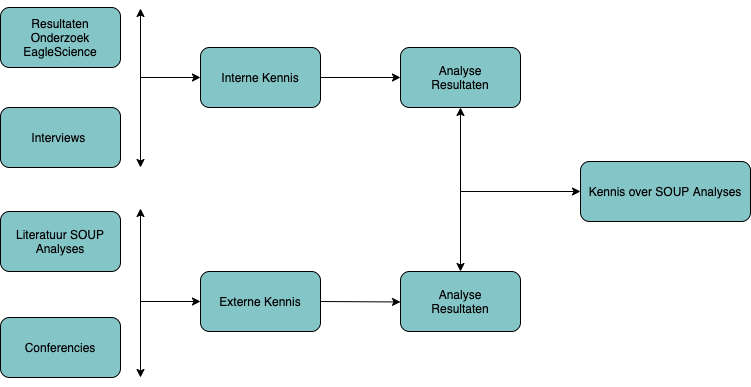
\includegraphics[width=10cm]{gfx/OnderzoeksmodelSOUP}
  \caption{Onderzoeksmodel SOUP analyse module}
  \label{fig:Onderzoeks model Dev-Stack}
\end{figure}

Veel kennis van buiten zal worden vergaard doormiddel van het lezen van artikelen en boeken over het onderwerp.
Hierbij moet worden gelet op de toepasbaarheid en scope van het artikel.

\section{Tijdsverloop Onderzoeken}\label{sec:tijdsverloop-onderzoeken}
Beide onderzoeken zullen parallel uitgevoerd worden zodat beide onderzoeken elkaar inzichten kunnen verschaffen en er op die manier een beter begrip van de mogelijkheden is.

%    \chapter{Onderzoek: Architectuur binnen Eaglescience}\label{ch:onderzoek:-architectuur-binnen-eaglescience} % Chapter title

%TODO: MarginPARS zetten
Dit hoofdstuk geeft het onderzoek weer naar de manier waarop EagleScience software ontwikkeld en uitrold. Er wordt ingegaan op de verschillende programeertalen en frameworks die in gebruikt zijn als ook de tooling die wordt gebruikt om de software daadwerkelijk te ontwikkelen en uitrollen.

%TODO: Vraag minder vaag maken denk ik ??
\section{Onderzoeksvraag}\label{sec:ESOnderzoeksVraag}
De onderzoeksvraag die als startpunt van dit onderzoek geld is: "Hoe wordt er binnen EagleScience software ontwikkeld en uitgerold en welke tooling wordt er gebruikt?". Deze onderzoeksvraag werpt een deelvragen op waar eerst een onderzoek naar gedaan dient te worden, waaruit vervolgens een conclussie kan worden getrokken en daarmee de hoofdvraag beantwoord.
\begin{itemize}
  \item Welk proces wordt er binnen Eaglescience gebruikt om software te ontwikkelen?
  \item Wat zijn de meest gebruikte ontwikkeltalen en frameworks die binnen EagleScience worden toegepast?
  \item Welke tooling wordt er gebruikt binnen EagleScience?
  \item Hoe wordt er binnen EagleScience software uitgerold?
\end{itemize}

\section{Requirements}
Blaat over requirements.
%
%\section{Hoe wordt er op het moment gewerkt binnen eagleScience?}\label{sec:hoe-wordt-er-op-het-moment-gewerkt-binnen-eaglescience?}
%Eaglescience werkt op project basis met klanten.
%Om project inzichtelijk te maken en beter te kunnen defineren wordt er gebruik gemaakt van een planning middels fasen die doorlopen worden.
%Iedere fase heeft een gedefineerd einde dat in overeenstemming met de klant wordt vastgelegd.
%Er is echter een uitzondering op de fase project maintenance waarbij Eaglescience gewenst onderhoud pleegt op de geleverde applicatie dan al niet met hosting.
%\medskip
%
%\textbf{Phase1: Sales \& acquisition}
%onderzoeksfase waarin vooral de wensen en restricutes vanuit de klant in kaart wordt gebracht.
%Hierbij kan gedacht worden aan: Doel van de applicatie met daarbij de requirements en restraints, planning, budget en hosting.
%Het resultaat is een inschattingsdocument met daarin informatie die het team verder helpt in het vormgeven van het project.
%
%\textbf{Phase2: Project initiation}
%In deze fase wordt het project opgestart.
%Er wordt een team samengesteld die gaat werken aan het ontwikkelen van de software.
%Deze fase is ook cruciaal om alle platform in gereedheid te brengen te denken aan rechten voor de ontwikkelaars op Azure Cloud, Sentri, Jenkins en dergelijke.
%Als alles in gereedheid wordt gebracht is er een project kick-off waarbij hetteam wordt ingelicht over het project en taken die vervult moeten gaan worden.
%
%\textbf{Phase3: Start \& Execution}
%Dit is een iteratieve fase die in sprints doorloopt tot het project gereed is.
%Waarbij na iedere sprint een demo wordt gegeven verdere uitweiding over deze fase is hieronder te vinden onder "Dagelijkse werkwijze"
%
%\textbf{Phase4: Project Warp up}
%In deze fase wordt het project opgeleverd aan de klant en wordt dan al niet door Eaglescience gehost op Azure cloud.
%Er wordt een project retro gehouden waarbij het team terugkijkt op de werkzaamheden en hoe deze verliepen, daarnaast is er een evaluatie met de klant.
%
%\textbf{Phase5: Project maintenance}
%Geen enkel software wordt direct zonder bugs opgeleverd deze fase duurt dan ook zolang de als software lifecycle is of tot het budget van de klant op is :D In deze fase wordt support geleverd door Eaglescience op de source code en mogelijk aanpassingen gedaan om bugs te verwijderen of performance te verbeteren.

\section{Dagelijkse werkwijze}\label{sec:dagelijkse-werkwijze}
Binnen Eaglescience wordt er getracht om "full Scrum" te werken. Dit wil zeggen dat voor ieder project een team van maximaal 9 full-stack developers wordt aangewezen. De sprints duren ongeveer 2 á 3 weken afhankelijk van wensen van de klant en beschikbaarheid van ontwikkelaars. Iedere sprint begint met een refinement waarbij de taken die op de backlog staan worden bekeken en ingeschat door het team. Tijdens de sprint vindt de ontwikkeling middels taken plaats die vervolgens worden gereviewd door een ander teamlid. Aan het einde van de sprint vind er een retrospective plaats en eventueel een demo om de voortgang te demonstreren aan de klant, dit is ook het moment dat het team ziet hoe de applicatie in het algemeen werkt. Dit is ook het moment voor de projectmanager en product owner om de taken die op de back-log staan opnieuw te prioriseren waarbij in de refinement van de volgende sprint de taken mee worden genomen.

Om deze werkwijze te ondersteunen maakt EagleScience gebruik van de een PO(T)AP(Personal, Development, (Test), Acceptence, Production) buildstraat. Alle genoemde omgevingen worden gehost in Azure Kubernetes en maken gebruik van docker containers. Iedere ontwikkelaar heeft zijn eigen omgeving die hij kan bouwen om te testen of aanpassingen werken zoals verwacht. Er is per project een Ontwikkelomgeving waarin getest wordt of alle aanpassingen van de ontwikkelaars met elkaar werken. De acceptatie omgeving is er voor de projectmanagers en testers vanuit de klant of desgewenst externe testers om de ontwikkelde applicatie te testen zoals hij naar productie zou gaan. De productie omgeving host alle applicaties die 'live' zijn. Gezien alle omgevingen in docker containers draaien zijn deze volitile en kunnen dus "makkelijk" worden vervangen. zeker voor de personal en development omgeving wordt dit gezien als een voordeel vanwege het vele bouwen van deze omgevingen.
\section{Ontwikkeltalen en tooling binnen EagleScience}\label{sec:ontwikkeltalen-en-tooling-binnen-eaglescience}
EagleScience maakt volledige full stack oplossingen. Er wordt dus zowel front-end, backend, en database oplossingen ontwikkelt binnen projecten. Er wordt dan gebruik gemaakt van een aantal ontwikkeltalen en frameworks om deze oplossingen te kunnen ontwikkelen. Naast de ontwikkeltalen zijn er ook een aantal tools die worden gebruikt door eaglescience om support te kunnen leveren en projecten te kunnen managen.

\subsection{OntwikkelTalen en frameworks}\label{subsec:ontwikkeltalen-en-frameworks}
\marginpar{backend} \marginpar{Scala}
De voornamelijkst taal voor het ontwikkelen van de backend binnen EagleScience is Scala. De keuze voor deze taal is de mogelijkheid om functioneel te kunnen programmeren en dat het in de Java Virtual Machine (JVM) draait. Dat laatste zorgt ervoor dat bibliotheken die geschreven zijn in talen die ook ondersteunt worden door de JVM gebruikt kunnen worden ongeacht of deze in Scala, Java, Groovy of Kotlin geschreven zijn. Daarnaast is Scala zeer geschikt om kleine applicaties te schrijven die vervolgens groeien. De naam Scala is een samenraapsel van 'Scalable Language'. Het feit dat binnen EagleScience functioneel geprogrameert. heeft te maken met een aantal eigenschappen van de op deze manier programeren:
\smallskip %TODO: Wellicht iets verder uitweiden over de beweegredenen van het gebruik van Scala en Play.
\begin{enumerate}
  \item functioneel programeren stelt de programeur in staat om code te schrijven dat voorspelbaarder is.
  \item makkelijker te testen is door het feit dat bij een pure functie de output altijd zeker is vanuit de input
\end{enumerate}
Binnen Scala worden er in bijna alle projecten een aantal frameworks/bibliotheken gebruikt die het ontwikkelen van microsaervice web applicaties makkelijk maakt:
\begin{itemize}
  \item \textbf{PlayFramework 2.xx} Een web framework voor de ontwikkeling van webapplicaties in Scala we gebruikten het vooral als router voor de verschillende microservices die er achterliggen.
  \item \textbf{ArchES} is een intern ontwikkeld framework wat de opbouw en de communicatie tussen microservices in scala verbeterd.\ ArchES is geinspireerd op Apache KAFKA en werkt middels hetzelfde pub -> sub principe.
\end{itemize}

B
Voor de front-end wordt gebruik gemaakt van Typescript



\begin{itemize}
\item \textbf{Scala 2.xx} is gekozen om functioneel programeren te ondersteunen maar ook de mogelijkheid om OOP methodieken te gebruiken.\ Daarnaast maakt scala gebruik van de JVM wat op zichzelf voordelen heeft in portabiliteit( code once run everywhere).\ Door op de JVM te draaien kan Scala ook gebruik maken van bibliotheken die op diezelfde JVM draaien gebruiken en daarmee dus ook bibliotheken die geschreven zijn in Java, Groovy of Kotlin.\\
Functioneel programeren is een manier van programeren dat zijn basis heeft in de wiskunde.\ Neem bijvoorbeeldde volgende functie: \(y = func(x)\) waarbij \(x\) de input voor een functie is.\ Uit deze functie komt altijd \(y\) bijvoorbeeld als de functie \(x+1\) is dan zal de waarde van \(y\) altijd 3 zijn als \(x\) 2 is.\ Dit is een zekerheid alsook de zekerheid dat er geen andere waarden als output zijn dan \(y\).\ Dit fenomeen wordt een pure functie\footnote{Pure functies hebben geen side-effects wat betekend dat het niets anders doet dan de output geven van de functie. een Console.log wordt gezien als een side-effect omdat dit naast de output ook een andere output heeft(namelijk naar het scherm). Meestal bestaat de kern (business logic) van een applicatie uit pure functies en is er een schil omheen gebouwd die niet puur is maar zorgt voor de I/O van de applicatie} genoemd.\ Enkele voordelen van het functioneel programeren zijn:
\begin{enumerate}
  \item functioneel programeren stelt de programeur in staat om code te schrijven dat voorspelbaarder is.
  \item makkelijker te testen is door het feit dat bij een pure functie de output altijd zeker is vanuit de input
\end{enumerate}
Daarnaast bestaat ook door een effect uit de wiskunde de muterende variable niet een waarde van een variable is altijd het zelfde en mocht deze toch gewijzigd moeten worden ( bijv.\ een e-mail adres van een gebruiker ) dan wordt de data in het programma opgeslagen in een nieuwe variabele waar vervolgens verder mee gewerkt wordt.\ Hiermee komt gelijk een nadeel van functioneel programeren.\ Als de applicatie veel data tegelijk muteerd dat kan de geheugen footprint groter worden dan bij een soort gelijke applicatie dat volgens het OOP principe is geschreven.\ Een ander nadeel is dat OOP op dit moment de defacto methode is om applicaties te schrijven en het omscholen naar functioneel programeren tijd kost.

De filosofie binnen Eaglescience is dat Scala helpt bij het bouwen van software waarbij de output vast staat aan de input en dus veel betrouwbaarder en voorspelbaarder wordt.\ Daarnaast wordt het testen, wat een eis is in alle projecten binnen Eaglescience, veel inzichtelijker wordt.

\item \textbf{TypeScript} TypeScript is een open-source taal wat gebouwd is op JavaScript maar met statische type definities toegevoegd, het voordeel is dat het lijkt op JavaScript echter door Types te gebruiken kunnen veel fouten worden ontdekt en opgelost bij het schrijven van de code in plaats van tijdens Run-time.\ Typescript is daarom de keuze van EagleScience om front-end applicaties te schrijven.\ Eaglescience gebruikt voornamelijk Angular voor de ontwikkeling van front-end applicaties.
\end{itemize}


\subsection{Tooling}
\begin{itemize}
\item \textbf{Jira} Is naar eigen zeggen (JiraWebsite ) de nummer 1 software ontwikkel tool voor agile teams.\ Eaglescience gebruikt het om projecten te plannen volgens de scrum methode.\ De tool maakt het mogelijk om sprints te plannen, en het bijhouden van projecten worden ondersteunt.
\item \textbf{Confluence}
Confluence wordt binnen Eaglsescience gebruikt als samenwerkings tool waarbij de documentatie centraal ligt.\ De omgeving bied de mogelijk om samen te werken met Jira waardoor documentatie makkelijk te vinden op zowel project als taak niveau.
\item \textbf{GitLab}
De Code Repository die Eaglescience gebruikt.
\item \textbf{Jenkins}
Jenkins is een open-source automation server wat door Eaglescience gebruikt wordt om projecten te builden voor verschillende doeleinden.\ Doordat Jenkins Open-source is zijn er veel plugins geschreven die de functionaliteit uitbreiden en het dus bruikbaar maakt voor het bouwen van een pipeline voor veel verschillende talen en frameworks.
Jenkins kan worden vergeleken als mission control tijdens de lancering van een raket\ Voordat de raket(de deploy) gelanceerd kan worden, wordt er een go-nogo sequence uitgevoerd waarbij iedere stap een test of check is waar alleen een go of no-go uit kan komen.\ Op het moment dat alles op go staat is de build geslaagd en kan er gedeployed worden.\ Wil niet zeggen dat de deploy altijd geslaagd is met Jenkins.\ Er zijn nog een aantal andere factoren die meehelpen aan een geslaagde deploy zoals bijvoorbeeld bugs die niet uit de tests zijn gekomen.
\item \textbf{Sentry}
Sentry is een errortracking solution welke Eaglescience gebruikt voor het ik kaart brengen van bugs en fouten die optreden in applicaties op productie en acceptatie omgevingen.\ Het bied de mogelijkheid om gedetaileerde informatie te krijgen over de fouten die optreden inclusief metadata als frequentie, ernst en gebuikers statistiscs zoals os, device, etc).
\item \textbf{Nagios}
Nagios is een intern monitoring systeem die de services die nodig zijn voor het dagelijks werken binnen eaglescience monitored en meldingen geeft als er iets mis gaat of freigd te gaan.\ Op basis van gegevens vanuit nagios kan automatisering en devops acties ondernemen om de services draaiend te houden.
\item \textbf{Azure Cloud}
Cloud omgeving van Microsoft waar we gebruik maken van verschillende services waaronder de Azure Kubernetes Service waar we docker containers draaien in pods voor productie.\ Daarnaast zijn er een aantal VM's waar ontwikkelen test omgevingen draaien.\ Azure maakt het ook mogelijk om logs bij te houden van de pods die draaien en daar dus metrics op kunnen uitvoeren waardoor we beter inzicht hebben in de performance van de applicaties in productie.\ Als inzicht in het gebruik ervan.\ Waardoor we betere service kunnen leveren richting de klant.
\end{itemize}

\section{Hoe wordt op dit moment software gedeployed?}\label{sec:hoe-wordt-op-dit-moment-software-gedeployed?}
Zoals hierboven berschreven wordt Jenkins gebruikt om software te deployen naar zowel de productie omgevingen alsook de verschillende development en acceptatie omgevingen.
Een deploy wordt gedaan op het moment dat er source code naar gitlab gepushed wordt.
Doormiddel van Tokens in de Commit message kan gestuurd worden waar de build(als deze slaagt) gedeployed wordt bijv: {-all + portal} build en deployed alleen de portal. [ci-skip] zorgt ervoor dat er alleen een push wordt gedaan en geen build wordt gestart.
De configuratie die Jenkins gebruikt wordt beschreven in een aantal Jenkins files die meegenomen worden de repo.
Naast de deploy geeft Jenkins nog een aantal andere waardevolle Artifacts als test/lint rapportages.
Een build en deploy gaat volgens de onderstaande afbeelding:

\begin{figure}[H]
\myfloatalign
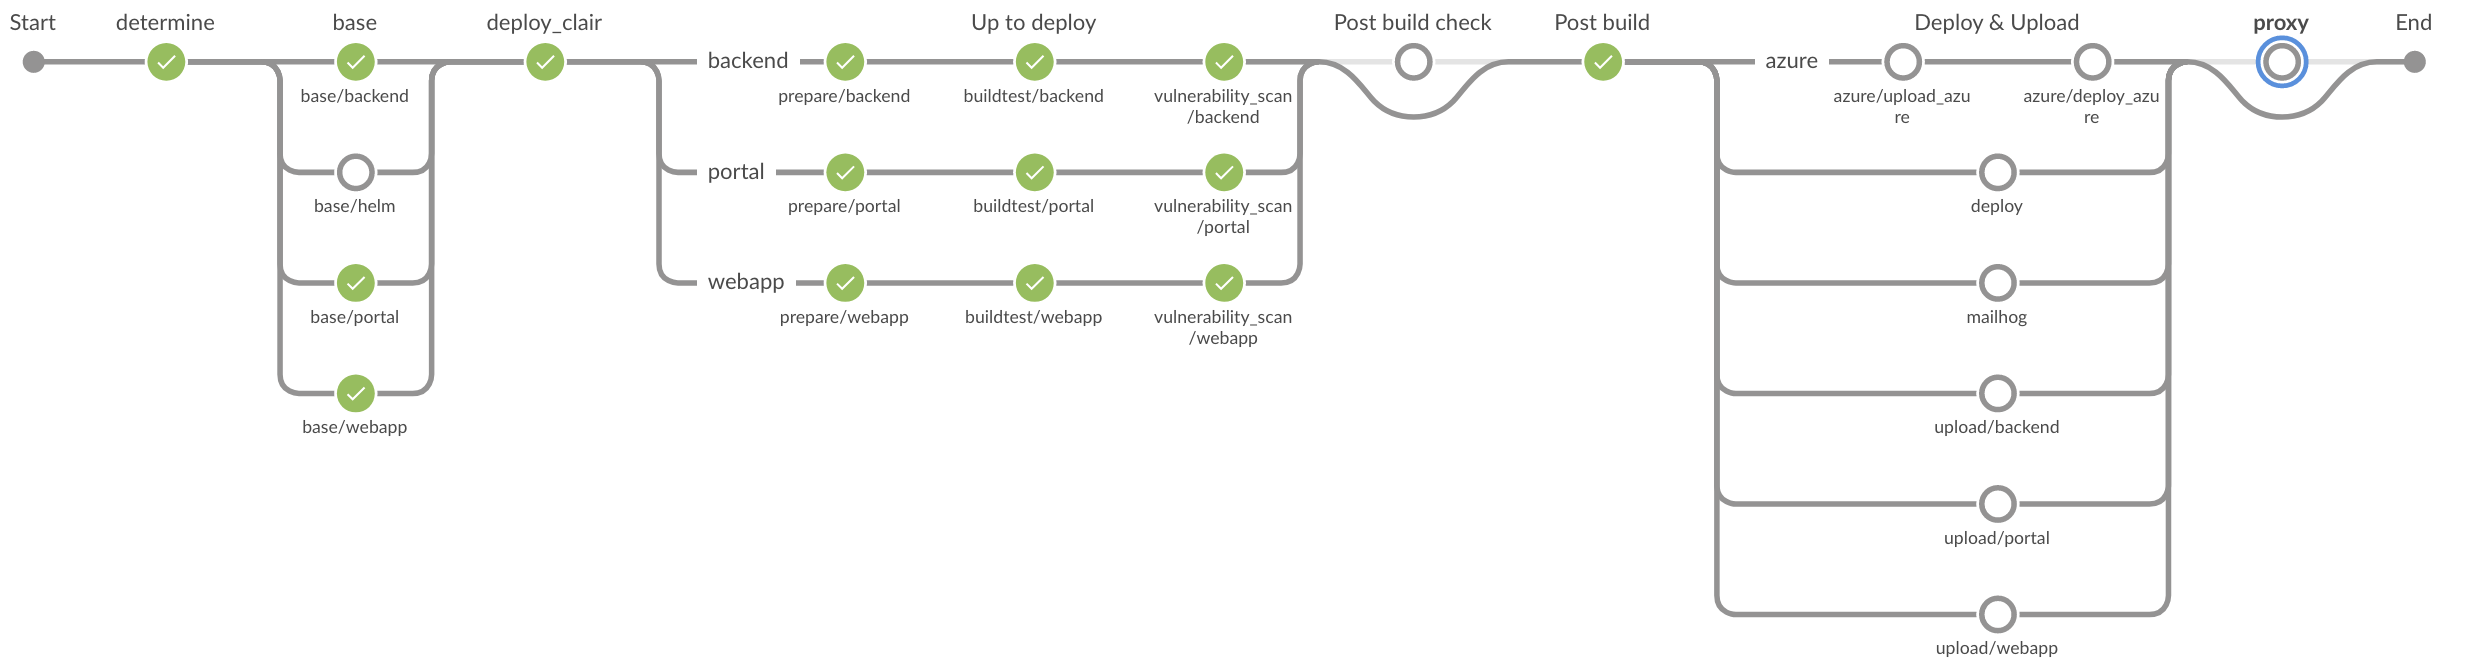
\includegraphics[width=15cm]{gfx/Screenshot 2021-08-18 Jenkins PipeLine}
\caption{Jenkins(Blue Ocean) pipeline}
\label{fig:JenkinsPipeLine}
\end{figure}
Een Jenkins pipeline werkt in een aantal stappen dat in een .jenkinsFile wordt beschreven.
Deze jenkinsFile wordt in de determine stap ingelezen en de benodigde stappen op een rij gezet.
De stappen die worden uitgevoerd zijn:
\begin{itemize}
\item \textbf{determine} Nu wordt bekeken welke stappen er nodig zijn om een succesvolle build en of deploy te kunnen doen./ Aan de hand van een JenkinsFile en tokens in een Commit message wordt hier bekeken welke stappen er moeten worden uitgevoerd om tot een goed einde te komen.
\item \textbf{base} In de base stap worden alle Containers voorbereid die nodig zijn om de applicatie te draaien.\ Images worden opgehaald en gedeployed De base stap is een parallel lopende stap waarin in dit geval backend, portal en de app worden voorbereid.
\item \textbf{deploy clair} de clair scanner zoekt op kwetsbaarheden binnen containers die zojuist zijn aangemaakt.\ Dit is een extra veiligheid die ervoor zorgt dat de images en container veilig zijn er alleen nog door bibliotheken die gebruikt worden voor ontwikkeling kwetsbaarheden kunnen worden toegevoegd
\item \textbf{Up to deploy}
in dit geval wordt er voor de backend, portal, en app een parallel process gestart waarin alle drie substappen doorlopen:
\begin{itemize}
\item \textbf{prepare} Docker containers worden ingesteld, en klaar gezet voor het ontvangen van de services.
\item \textbf{builtest} De services worden gebuild en gestest in deze stap.\ Eaglescience heeft een aantal tresholds opgesteld waaraan tests moeten voldoen om deze te analyseren worden de test resultaten vanuit de docker containers gekopieerd naar de Jenkins Store waar Jenkins de waarden kan analyseren als alle tests binnen de resultaten vallen wordt de volgende stap uitgevoerd.
\item \textbf{vulnerability scan} Clair scanner scant nu de containers nogmaals maar nu op de gebruikte software.\ Als clair iets vind dat eaglescience als verdacht acht dan wordt de build gestaakt.
\end{itemize}
\item \textbf{PostBuild(check)}
Alle bevindingen worden hier gecheckt mocht er iets mis zijn wordt er wederom afgebroken en is de build gefaald en kan er dus niet een deploy plaatsvinden.
\item \textbf{Deploy \& Upload}
in dit geval wordt de deploy niet uitgevoerd.\ Deze stap zorgt ervoor dat de gebouwde containers worden overgedragen naar Azure.\ Iedere container heeft wederom zijn eigen stappen.
\item \textbf{End}
Einde van de PipeLine Jenkins geeft de workers die het project heeft gebruikt weer vrij.
\end{itemize}

    % Todo Betere titel vinden
\chapter{Onderzoek: Externe bibliotheken gebruiken en het gevaar hiervan}\label{ch:onderzoek:-SOUP-analyse}
Dit hoofdstuk beschrijft het onderzoek wat gedaan is om meer inzicht te krijgen in het doen van een SOUP-analyse. Als eerst wordt de onderzoeksvraag ontleed in te beantwoorden deelvragen. Daarna zal er wordt iedere deelvraag beantwoord om vervolgens tot een conclusie te komen welke de onderzoeksvraag beantwoord.

\section{Onderzoeksvragen} \label{sec:SOUPOnderzoeksvragen}
De onderzoeksvraag die als startpunt van dit onderzoek geld is:"Hoe kunnen we externe bibliotheken op een veilige manier gebruiken?" of "Hoe kan SOUP op een effectieve manier worden geanalyseerd en hoe maakt dit software veiliger?". Uit deze hoofdvraag kunnen de volgende deelvragen worden ontleed:
\begin{itemize}
    \item Wat is SOUP?
    \item Wat dragen externe bibliotheken en dus ook potentieel SOUP bij aan de ontwikkeling van software?
    \item Wat zijn de gevaren van het gebruik van SOUP?
    \item Wat relateert SOUP tot software veiligheid binnen EagleScience?
\end{itemize}

%Goed verhaal over supplychain Attacks : https://learning.oreilly.com/library/view/alice-and-bob/9781119687351/c01.xhtml#head-2-27

\section{Software of unkown provenance}\label{sec:software-of-unkown-provenance}

\subsection{Wat is Software of Unkown Provenance(SOUP)?}\label{subsec:wat-is-soup?2}
De term SOUP komt oorspronkelijk de wereld van de ontwikkeling van medische software en staat voor "Software Of Unkown Provenance".
SOUP wordt gezien als een software component dat al ontwikkeld is en beschikbaar is gesteld voor gebruik door een instantie anders dan de gebruiker zonder dat de bewijzen zijn over de manier van ontwikkeling als de kwaliteit van de software.
Hierdoor is het dus niet duidelijk welk process er is gevolgt tijdens het ontwikkelen en daarmee dus ook de (medische)veiligheid niet is aan te tonen.
De term wordt nu steeds vaker gebruikt in de algemene software ontwikkel kringen om aan te geven dat er van een betreffent software component(framework, bibliotheek, etc.) niet bekend is hoe het ontwikkeld, getest is.
Hierdoor is er dus geen zekerheid dat het component kwetsbaarheden kan bevatten.
Kwetsbaarheden in deze zin zijn dan voornamelijk lekken of veranderingen van functionaliteiten binnen een software.
\subsection{Hoe relateert SOUP zich met het ontwikkelen van veilige software?}
Om deze vraag te kunnen beantwoorden moeten we eigenlijk twee zaken onderzoeken als eerste  Waarom gebruiken we soup en ten tweede wat wordt er gedaan om veilige software te ontwikkelen.

De voornaamste redenen om bibliotheken te gebruiken is het verminderen van het herhaaldelijk schrijven van code om basis functionaliteiten in een applicatie te krijgen. En Daarmee wordt de ontwikkeltijd verminderd. Het gebruik van bibliotheken is tegenwoordig niet meer weg te denken uit de ontwikkelstrategie van een bedrijf. Deels omdat er een standaard is waarmee gewerkt wordt, wat op zijn beurt het aannemen en opleiden van personeel vergemakkelijkt. Daarnaast hebben veel gebruikte bibliotheken een 'community' waar vragen gesteld kunnen worden om zo moeilijkheden te verminderen. Een nadeel zoals hierboven is beschreven is dat het niet altijd duidelijk is hoe veilig een bibliotheek is.

\section{Veilig software schrijven?}
veilig software schrijven is niet altijd even makkelijk. Er zijn meerdere redenen waarom er niet veilige software wordt geschreven. Tijd en budget zijn vaak de oorzaak omdat software snel op de markt moet komen en er dus niet genoeg tijd gereserveerd wordt om te onderzoeken of er bugs en kwetsbaarheden bevinden. Een tweede mogelijkheid is dat er niet genoeg kennis is om daadwerkelijk veilige software te schrijven. Een andere mogelijkheid is dat er kwaadwillend bewust kwetsbaarheden in bibliotheken worden geschreven om zo een achterdeur te hebben om aanvallen of diefstallen te doen.
In het tweede geval zijn er meerdere instanties die het bouwen van veilige software als doelstelling hebben en er veel aan doen om ontwikkelaars wereldwijd te onderwijzen in goed gebruiken. Eén van de belangrijkste is de OWASP(OWASP.org) de OWASP heeft een aantal projecten die ontwikkelaars in staat stellen om veiligere software te ontwikkelen. Eén daarvan is de OWASP top 20 die ongeveer iedere 5 jaar uitkomt. Dit jaar is er een nieuwe top 10

omlaag brengen van ontwikkeltijd. En het herhaaldelijk moeten schrijven van code. Voor veel basis taken die een applicatie zou moeten uitvoeren is veelal een bibliotheek geschreven die deze taken prima uit kan voeren.


%Bron: "https://johner-institute.com/articles/software-iec-62304/soup-and-ots/"

\section{Hoe kan het gebruik van SOUP gevaarlijk zijn?}\label{sec:hoe-kan-het-gebruik-van-soup-gevaarlijk-zijn?}
Uit een onderzoek van Contrast Security blijkt dat 80\% van de broncode die vandaag de dag gebruikt wordt om een applicatie te schrijven bestaat uit broncode uit een externe bibliotheek.
Waarbij een vierde van de gedownloade bibliotheken kwetsbaarheden bevatten.
De kans dat er dus onbekende kwetsbaarheden in een applicatie sluipen is dus zeker aanwezig.
Een van de redenen dat dit kan gebeuren is een fenomeen dat een package dependency network wordt genoemd.
Wat in het kort betekend dat een dependency die je als ontwikkelaar gebruikt zelf ook een aantal dependencies heeft, welke op zijn beurt ook weer dependecies heeft.
[verder uitwerken]
Dit kan in theorie vele lagen bevatten waardoor de structuur minder inzichtelijk wordt omdat er voor iedere dependency in het netwerk een assesment gedaan moet worden naar kwetsbaarheden.
In verschillende artikelen(Bronnen) wordt gewaarschuwd voor het gevaar van het gebruik deze constructie, echter lijkt het erop dat er binnenkort niet echt verandering komt in de manier waarop dependencies worden gelinkt.
Een andere oplossing zou dan zijn om iedere depenency te checken op kwetsbaarheden tegen een database
Bron: On the inpact of security vulnerabilities in npm package dependency network - Alexandre Decan, Tom Mens, Eleni Constantinou (2018), Structure and Evolution of package dependency networks.

\section{Instanties en SOUP}\label{sec:instanties-en-soup}
Kwetsbaarheden binnen softwareontwikkeling is niet iets van de laatste tijd en er zijn gelukkig instanties die zich bezig houden met het veilighouden van software door middel van trainingen, lezingen en andere manieren van awareness opwekken.
Sommige instanties houden bij welke kwetsbaarheden er gevonden zijn en plaatsen dit in een CVE-database.
Anderen melden veel voorkomende kwetsbaarhden in een top-10

\subsection{CVE Databases, MITRE, NIST, NVD}\label{subsec:mitre-nist-nvd}
CVE staat voor Common Vulenerabilities en Exposures wat een database waarin kwetsbaarheden staan die gevonden zijn in de verschillende systemen.
Deze Database wordt voornamelijk bijgehouden door het bedrijf MITRE dat met subsidie van de US Division of Homeland Security werkt aan het kenbaar maken van lekken in software\footnote{Software wordt hier gezien in de ruimste zin van het woord hierbij hoort: Operating systems, open en closed source software. maar ook frameworks en bibliotheken.}.
De CVE's die in deze database staan worden vervolgens geannalyseerd door het NIST(National Institute os Standards and Technology) en voorzien van een CVSS\footnote{Common Vulnerability Score System is een gestandardiseerde manier om een score aan een kwetsbaarheid toe te kennen waarop in een enkel oog opslag te zien is hoe rieel een risico is.} score en geplaats in de NVD-database.
Zowel de database van MITRE (https://cve.mitre.org) als NIST (https://nvd.nist.gov) zijn publiekelijk toegankelijk.

\subsection{OWASP}\label{subsec:owasp}
Naast het bijhouden van CVE's in database is het creëren van awareness net zo belangrijk.
Een instantie die zich bezig houd hier mee is OWASP(Open Web Application Security Project) die awareness creëert door ideree 5 jaar\footnote{helaas is op het moment van schrijven de laatste versie(2021) nog niet uitgebracht en staat hier de versie uit 2017} een Top-10 uit te brengen met daarin de meest voorkomende en dreigende kwetsbaarheden die ze gevonden hebben in een dataset wat opgebouwd is uit inzendingen van 500+ onderzoekers van 40+ bedrijven die samen meer dan 100.000 API's en web applicaties hebben onderzocht.
In de top 10 die hieronder samengevat weer wordt gegeven wordt er een score meegegeven over hoe makkelijk een lek is te ontdekken en welk mate van risico de kwetsbaarheid heeft.

\begin{figure}[H]
    \myfloatalign
    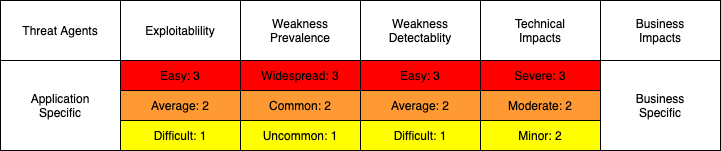
\includegraphics[width=12cm]{gfx/risk tabel}
    \caption{Inschaling van risico's door OWASP}
    \label{fig:risico inschaling}
\end{figure}

\begin{itemize}
%Bron: https://codebros.nl/blog/wat-is-de-owasp-top-10 , https://owasp.org/www-project-top-ten/ << PDF download

    \item \textbf{A01:2017 Injection[exploitabity: 3, Prevelance: 2, detectability: 3, technical: 3]:}

    De mogelijkheid om OS, SQL, NoSQL commandos te injecteren in web applicaties zorgt ervoor dat aanvallers toegang kunnen hebben tot delen van systemen zonder er recht op te hebben.
    Daarnaast is er ook de mogelijkheid om toegang te krijgen tot data die niet voor hen bedoelt is.


    \item \textbf{A02:2017 Broken Authentication[exploitabity: 3, Prevelance: 2, detectability: 2, technical: 3]:}

    Het verkeerd implementeren van authentication en session management kan er voor zorgen dat aanvallers wachtwoorden, sessie tokens aan kunnen passen om zo zich voor te doen als een andere gebruiker.

    \item \textbf{A03:2017 Sensitive Data Exposure[exploitabity: 2, Prevelance: 3, detectability: 2, technical: 3]:}

    Het verkeerd of niet voldoende afschermen van API's kunnen ervoor zorgen dat sensitive data makkelijk gevonden kan worden.\ Zeker als de data niet encrypted verzonden wordt.

    \item \textbf{A04:2017 XML External Entities (XXE)[exploitabity: 2, Prevelance: 2, detectability: 3, technical: 3]:}

    Veel oude of slecht geconfigureerde XML-processoren evalueren externe entiteit referenties binnen XML-documenten slecht.\ Hierdoor is het mogelijk om links te creeën naar bestanden en/of fileshares waar code staat die slecht is voor de applicatie [that contains malicious code].

    \item \textbf{A05:2017 Broken Access Control[exploitabity: 2, Prevelance: 2, detectability: 2, technical: 3]:}

    Beperkingen op wat een geauthenticeerde gebruikers mogen worden niet altijd nageleefd, Aanvallers kunnend deze fouten gebruiken om toegang te krijgen tot gegevens of functionaliteiten die niet bestemd zijn voor deze gebruikers.\ Ze kunnen gegevens aanpassen en / of toegangsrechten aanpassen.

    \item \textbf{A06:2017 Security Misconfiguration[exploitabity: 3, Prevelance: 3, detectability: 3, technical: 2]:}

    Slechte configuratie van de veiligheids instellingen zijn de meest gevonden probleem.\ Dit is meestal het gevolg van het gebruiken van de default, incomplete of ad hoc configuratie Hierdoor kunnen cloud storages open komen te staan, verkeerd geconfigureerde HTTP-headers of foutmeldingen die te veel informatie meegeven ontstaan.

    \item \textbf{A07:2017 Cross-Site Scripting (XSS)[exploitabity: 3, Prevelance: 3, detectability: 3, technical: 2]:}

    Middels XSS is het mogelijk om scripts te draaien van een andere bron dan wenselijk.\ Dit geeft de mogelijkheid om via een browser andere scripts in de applicatie te draaien zo proberen andere functionaliteiten toe te voegen.\ Wat kan leiden tot een web-site dat zich anders gedraagt dan de bedoeling is.

    \item \textbf{A08:2017 Insecure Deserialization[exploitabity: 1, Prevelance: 2, detectability: 2, technical: 3]:}

    Door het niet veilig serialiseren van objecten naar text kan het voorkomen dat er code of commando's mee worden gestuurd welke uitgevoers kunnen worden op de server.

    \item \textbf{A09:2017 Using components with Known vulnerabilities[exploitabity: 2, Prevelance: 3, detectability: 2, technical: 2]:}

    Componenten zoals bibliotheken, frameworks en andere software modules die gebruikt worden voor het ontwikkelen van een applicatie kunnen bedoeld of onbedoeld kwaadaardige code bevatten Wat kan leiden tot verschillende mogelijkheden voor de aanvaller binnen te dringen.\ Of data te versturen naar een andere host om zo achter "beveiligde" gegevens te komen.

    \item \textbf{A10:2017 Insuffivient Logging \& Monitoring[exploitabity: 2, Prevelance: 3, detectability: 1, technical: 2]:}

    Logging en monitoring is bijna net zo belangrijk als het ontwikkelen van een veilige applicatie, mocht er toch een aanval plaatsvinden op welke manier dient er de mogelijkheid zijn om terug te zien wat er precies gebeurt is.\ Logging zorgt hiervoor.\ Het monitoring deel is het bekijken van de logs om te zien of er iets verdachts plaats heeft gevonden.\ Er zijn tools beschikbaar die er voor automatische monitoring zorgen( Nagios is dit soort tool)

\end{itemize}

%Bronnen:
%https://www.imperva.com/learn/application-security/cve-cvss-vulnerability/
%http://owasp.org
\section{Invloed van SOUP op veiligheid van software}\label{sec:invloed-van-soup-op-veiligheid-van-software}
In de OWASP top-10 staat op plaats 9 "Using components with known vulnerabilities" wat aangeeft dat het op het moment van schrijven aandacht nodig heeft.
Eén van de redenen dat dit probleem in de top 10 staat is omdat het gebruik van bibliotheken bijna niet te vermijden is in de ontwikkeling van applicaties wat vooral te danken is aan het steeds sneller moet leveren van een product.
Ontwikkelaars zijn nooit volledig op de hoogte van de werking laat staan wie de onwikkelaar is van een externe bibliotheek.
Een goed voorbeeld hiervan is de "event-stream vulnerability" waarbij de bibliotheek voorzien werd van crypto-coin-stealing malware.
Dit kon gebeuren omdat de bibliotheek niet meer actief werd onderhouden en een persoon zich aanmelde om de ontwikkeling over te nemen.
Vervolgens werd een dependency omgezet van versie en functionaliteit waardoor er toegang werd, verleent om crypto coins te stelen.
Event-stream is een bibliotheek dat veel gebruikt werd als dependency voor applicaties de stream-functionaliteiten van nodejs gebruikten daardoor heeft het de potentie gehad om veel schade aan te richten.
Het is niet geheel duidelijk hoeveel schade er is gelden echter laat dit voorbeeld duidelijk zien wat het probleem is en hoe snel je kan verdwalen in dependency tree's.
Een oplossing is om regelmatig te scannen naar verdachte bibliotheken in de dependency tree.
En er vervolgens actief mee om te gaan door bibliotheken up-to-date te houden.
%Bron: https://www.theregister.com/2018/11/26/npm_repo_bitcoin_stealer/

\section{Dependency trees?}\label{sec:dependency-trees?}
Een dependency tree is een boom structuur waarin staat welke bibliotheken er gebruikt worden door een applicatie en kan beschikken over meerdere lagen.
Laten we als voorbeeld het boven genoemde "event-stream" npm package nemen.
Op de npm website staat vermeld dat deze package ondersteuning biedt aan 1895 andere pakketten en zelf 7 dependencies heeft.
Nu moet je als je zeker wil weten of er kwaadwillende broncode deze ook scannen.
Als we kijken hoeveel dependencies deze weer hebben komen op 4 depenendies die ieders weer dependencies hebben.
De tree van Event-stream is hier te vinden, de kwaadaardige package waar het mis mee ging is verwijderd uit de dependency tree door waarschijnlijk een andere oplossing te vinden.

\begin{figure}[H]
    \myfloatalign
    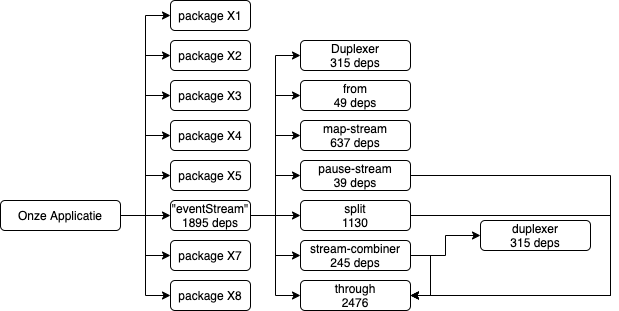
\includegraphics[width=12cm]{gfx/dependency-tree}
    \caption{Dependency tree}\label{fig:dependency-tree}
\end{figure}
Een applicatie heeft niet één zo'n boom maar voor iedere package in de eerste kolom bestaat zo'n boom die dus nog dieper kan gaan dan de hier afgebeelde.
Handmatig scannen is dus geen optie.
Dus moet de oplossing gezocht worden in het autmatisch scannen, gelukkig bestaan er een aantal scanners voor NPM depencies, zxoals versions en retire.js.
Maar ook voor Java en .NET bestaat er een dependency checker ontwikkeld door de OWASP\@.


[NOTE Volgende komt uit SOUP ANALYSE hoofdstuk]

\begin{itemize}
    \item https://jeremylong.github.io/DependencyCheck/
\end{itemize}

Voordat we verder kijken naar mogelijkheden om kwetsbaarheden in een externe bibliotheek te onderzoeken en te verhelpen moeten we eerst kijken naar een aantal kernbegrippen om te begrijpen waar het om gaat.

Dit onderzoek heeft daarom ook twee hoofdvragen die ieders weer een aantal deelvragen opwerpen.
Als eeste is de vraag "Welke kwetsbaarheden bestaan er hoe is het gebruik van externe bibliotheken hier aan gecorreleerd?
De deelvragen die hier uit voorkomen luiden:
\begin{itemize}
    \item Wat zijn applicatie veiligheidsrisico's?
    \item Welke komen het meest voor?
    \item
\end{itemize}

\section{Wat zijn applicatie veiligheidsrisico's}\label{sec:wat-zijn-applicatie-veiligheids-risico's}
Veiligheids risico's binnen applicaties zijn een som van kwetsbaarheden die zich bedoeld of onbedoeld in de applicatie bevinden, de vindbaarheid en de "schade" die er mee aangericht kunnen worden.
De termen van de som worden hieronder verder uitgediept als ook een top-10 uitgeven door de OWASP van de meest voorkomende kwetbaarheden.

Een aanvaller kan op meerdere manier in een applicatie komen(figuur X).
Vaak gebeurt dit door een kwetsbaarheid van een applicatie te zoeken en deze te exploiteren.
Als er vervolgens geen maatregeling genomen zijn om de aanvaller te weerhouden kunnen er zaken als data in een database, assets van het bedrijf of zelfs functionaliteit aangetast worden.
Wat op zijn beurt weer voor een impact in de bedrijfsvoering kan veroorzaken.
Hoe aanvallers een applicatie kunnen aanvallen is applicatie specifiek
De impact op de bedrijfsvoering is ook specifiek
\begin{figure}[H]
    \myfloatalign
    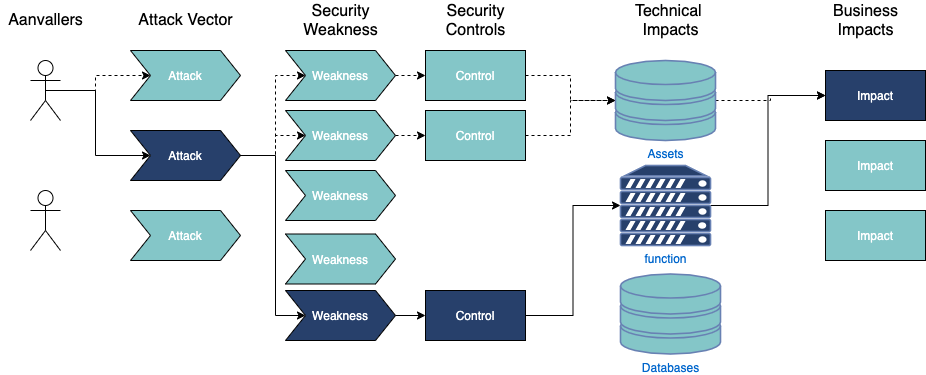
\includegraphics[width=15cm]{gfx/application security routes}
    \caption{Aanvalllen, en hun gevolg}
    \label{fig:Application Security Routes}
\end{figure}

Veiligheids risico's kunnen in categoriën worden geplaatst middels een gradatie systeem die in figuur x te ze zien is.
De OWASP-Top10 die verder in de tekst te vinden is maakt gebruik van dit gradatie systeem om risico's in te schalen.
OWASP is een instantie die zich bezighouden met het verbeteren van de veiligheid van applicaties.
Het doet dit door onder andere training en erkenning te geven aan kwetsbaarheden.
Zo wordt er eens in de 5 jaar een top-10 samengesteld met de op dat moment meest voorkomende kwetsbaarheden.
\footnote{Helaas is de laatste versie die aan het einde van 2021 uit moet komen nog niet beschikbaar op het moment van schrijven}
De OWASP-Top10 wordt samengesteld uit data van meer dan 100.000 productie applicaties en APIs wat door meer dan 500 mensen is getest door 40 verschillende bedrijven.
De top 10 is een aggegratie van deze data in de meest voorkomende issues met inachtneming van exploitabity, detectability en impact.


%\begin{figure}[H]
%  \myfloatalign
%  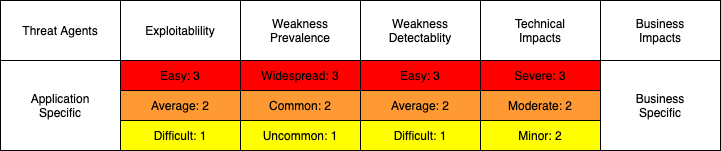
\includegraphics[width=12cm]{gfx/risk tabel}
%  \caption{Inschaling van risico's}
%  \label{fig:risico inschaling}
%\end{figure}

%threat agents = aanvallende entiteit
%exploitabity = exploiteetbaatheid
%weakness prevalance = vookomendheid van de zwakte in een applicatie
%weakness detectability = hoe goed is de zwakte in een applicatie te detecteren
%technical impact = technische impact op de applicaties
%business impacts = (zakelijke impact) impact op de bedrijfsvoering




In het vorige hoofdstuk is te lezen dat Eaglescience gebruik maakt van de volgende technologi\"en: Scala 2.XX, TypeScript, Jenkins, Docker ,Azure cloud.

Dit onderzoek richt voornamelijk op kwetbaarheden in bibliotheken  van derden en de bestrijding ervan.
En specifiek op de bovenstaande door Eaglescience gebruikte technieken.
De hoofdvraag voor dit hoofdstuk luid dan ook: "Met welke kwetsbaarheden hebben we te maken binnen Eaglescience en hoe kunnen we deze opsporen op een automatiseerde manier zonder de huidige werkwijze te verstoren?" Uit deze hoofdvraag onstaan de volgende deelvragen die in dit onderzoek beantwoord worden met daarna een conclusie op de hoofdvraag.

\begin{itemize}
    \item Welke soorten kwetsbaarheden zijn er?
    \item Hoe kunnen deze kwetbaarheden hun weg vinden in onze gebouwde software?
    \item Zijn er instanties die bijhouden waar zich kwetsbaarheden schuilhouden?
    \item Wat zijn methodes om te onderzoeken of er in de bestaande software kwetbaarheden bevinden?
    \item Is er een mogelijkheid om een third-party pakket in te zetten om dit te doen?
\end{itemize}

\

Binnen Eaglescience wordt er heel goed gekeken naar de manier waarop er veilige software ontwikkeld wordt.
Zaken die in de OWASP top-10 staan wordt serieus mee omgegaan en actief tegen gehandeld. zo wordt er ook gegekeken naar het gebruik van bibliotheken van derden.

Op plaats A09:2017 is te vinden dat er kwetsbaarheden middels bibliotheken van derden binnen kunnen komen. Dit is iets wat deels buiten het bereik van Eaglescience ligt. Om ons hier tegen te beschermen is het wenselijk om periodiek en geautomatiseerd een analyse naar kwetbaarheden tedoen.

De bibliotheken die gebruikt worden van derden wordt ook wel Software of unkown pedigree genoemd of kortweg SOUP. Dit houdt in dat een bibliotheek wordt ontwikkeld middels een proces of methode wat niet bekend is bij de eindgebruiker. Ook zijn vaak de details niet bekend van de bibliotheek omdat deze niet of nauwelijks wordt gereviewed door de eindgebruiker. Om deze reden is het dus onbekend of er kwetsbaarheden zitten in betreffende bibliotheken.
De definitie van SOUP blijft niet alleen bij de bibliotheken en frameworks vanuit het open-source gebied. Veelal is ook niet bekend hoe closed-source (Proprietary software) wordt geschreven, echter door reputatie van bedrijven die deze software schrijven wordt veelal , onterecht\footnote{zie: https://www.nu.nl/tech/6097701/waarom-de-hack-bij-solarwinds-ministeries-en-grote-bedrijven-treft.html } aangenomen dat deze geen lekken bevatten.

\section{CVE}
in de appliction security wordt er gesproken van een CVE(Common Vulnerability en Exposures) als een kewtsbaarheid bekend is deze wordt in een database geplaatst zodat \'e\'en ieder die geintreseerd is hier kan vinden welke software(os, applicatie, framework, bibliotheek) mogelijk niet veilig is. Deze Database wordt in stand en bijgehouden door een aantal instanties waarbij de belangrijksten zijn:
\begin{itemize}
    \item \textbf{NIST-CSRC} Computer Security Research Center van het National Institute of Standards and Technology) is een centrum dat onderzoek doet namens de Amerikaanse regering naar veiligheden in software. De database die het NIST-CSRC bijhoud heet het NVD(National Vulnerability Database) waarin CVE's worden bijgehouden.
    \item \textbf{CVE-Mitre} is een community driven effort wat CVE's logt in een lijst die vervolgens de NVD voedt met hun gevondendata.
    \item \textbf{cvedetails.com/}
    \item \textbf{vuldb.com/}
    \item \textbf{https://www.exploit-db.com/}
\end{itemize}

\section{}

https://www.security.nl/posting/666663/Van+CVE+tot+CVSS\%3A+wegwijs+in+het+woud+van+kwetsbaarheden










\section{Zijn er instanties die bijhouden waar zich kwetsbaarheden schuilhouden?}

Naast OWASP zijn er nog een aantal instanties dit bijhouden welke software\footnote{zoals hier gebruikt in de bereedste? zin van het woord dus: (Operating systems, ontwikkeltalen/databases, ontwikkelframeworks,bibliotheken) }
mogelijk kwetsbaarheden kunnen bevatten.
\begin{itemize}
    \item test
\end{itemize}


\section{Wat zijn methodes om te onderzoeken of er in de bestaande software kwetbaarheden bevinden?}

\section{Is er een mogelijkheid om een third-party pakket in te zetten om dit te doen?}

    % Chapter X





\chapter{Onderzoek: SOUP analyse}\label{ch:onderzoek:-soup-analyse} % Chapter title
Bronnen:

\begin{itemize}
    \item https://medium.com/@manjula.aw/nodejs-security-tools-de0d0c937ec0
    \item
\end{itemize}
\begin{itemize}
    \item Javascript     https://github.com/RetireJS/retire.js
    \item SBT https://github.com/albuch/sbt-dependency-check
    \item
\end{itemize}

%TODO: MarginPars zetten
Dit hoofdstuk geeft het onderzoek naar een methode om vanuit de projecten inzicht te krijgen in bekende kwetsbaarheden binnen gebruikte bibliotheken, en platformen. Er wordt ingegaan op welke tooling er beschikbaar is voor de verschillende onderdelen die we als EagleScience maken: Backend, frontend, Databases, Docker(containers). Daarna wordt er een selectie gemaakt voor de meest geschikte tool binnen de huidige buildstraat. Als laatst wordt er met de geselecteerde tooling een methode opgezet die het mogelijk maakt om gegevens uit de tooling in de portal te krijgen.

\section{Onderzoeksvraag}\label{sec:onderzoeksvraag}
De hoofdvraag in dit onderzoek is:  "Welke methodes zijn er beschikbaar voor het analyseren van kwetsbaarheden in bibliotheken van derden en welke het meest geschikt is voor het doel dat de opdrachtgever voor ogen heeft? ". Uit deze vraag komen een aantal deelvragen die ieders in een sectie hieronder wordt beantwoord.
Deelvragen:
\smallskip
\begin{itemize}
    \item Wat zijn de eisen waaraan de tool moet voldoen?
    \item Welke soorten tooling bestaan er?
    \item Welke tooling is er beschikbaar, wat zijn de voor en nadelen?
    \item Uit de gevonden tooling welke is het beste te integreren in de huidige pipeline/workflow?

\end{itemize}

\section{requirements}
De Opdracht luid dat er gescanned moet worden op actieve en niet actieve projecten op kwetsbaarheden. ER moet dus een methode komen die zowel periodiek een scan kan uitvoeren op projecten die niet meer actief in ontwikkeling zijn en een 'getriggerde' scan op het moment dat er bij een actief project code wordt toegevoegd en/of gewijzigd. Daarnaast moet de output van een suite te integreren zijn in de portal voor een ieder die hier belang bij heeft en de rechten bezit.



\section{Zoeken naar tooling}
Er zijn veel tools beschikbaar die helpen met het veiliger maken van software. De tools zijn te verdelen in twee typen:
\begin{enumerate}
    \item Suites zijn volledige pakketen die de gebruiker is staat stelt om inzicht te krijgen in de huidige staat van de geschreven source code. Hier kan worden gedacht aan slechte geschreven code(codesmells), linting maar ook security issues. Suites maken gebruik van plugins om verschillende taken te kunnen uitvoeren en of te scannen. en dit maakt ze hoog configureerbaar op het moment dat er een plugin bestaat voor de te analyseren ontwikkeltaal/systeem.
    \item Command line tools die specifiek op een onderwerp scannen. De voodelen van deze manier is dat het makkelijk ergens in een bestaande oplossing is in te bouwen en dat deze tools over het algemeen goed configureerbaar zijn. Een nadeel kan zijn dat het tijd kan kosten om de gewenste output te verkrijgen en deze vervolgens 'mooi' weer te geven in een applicatie.
\end{enumerate}
Gezien er deze twee smaken zijn moet er gekeken worden welke van de twee het beste past is de workflow van EagleScience met in achtneming de requirements die opgelegd zijn door de opdrachtgever.

\subsection{suites}
Veel bedrijven houden zich bezig met het veiliger maken van software en er is een ware markt ontstaan in suites om hierbij te helpen. Bedrijven als Snyk, SonarSource, Veracode, Synopsis brengen suites uit die het mogelijk maken om applciaties te annalyseren met gebruik van zowel source als compiles code. Een naardeel is zoals eerder genoemd is dat veel van deze suites gespecialiseerd zijn in een enkele taal of middels plugins andere talen kunnen ondersteunen. Daarnaast zijn veel bedoelt om code quality omhoog te brengen om op die manier veiliger en betere software te maken. Het zoeken naar kwetsbaarheden in bibliotheken van derden is meestal een extra feature. Een ander nadeel is dat veel van deze pakketen onder een license vallen en er vaak veel voor betaald moet worden. En gezien het budget voor EagleScience niet heel groot is lijkt het voor de hand liggend om een andere weg te kiezen.
\subsection{Commandline tooling (CLI's)}
Commandline tooling is een manier van tooling dat zich zeer geschikt maakt om te integreren in een bestaande build pipeline. Veelal zijn CLI's ook configureerbaar in de mate hoever ze moeten scannen en welke output ze waar moeten geven. Omdat CLi's makkelijker te ontwikkelen zijn dan complete suites zijn er vaak voor iedere ontwikkeltaal wel een scanning tool beschikbaar.
\subsection{Conclussie}
Uit de voor en nadelen die hierboven zijn genoemd kan worden geconcludeerd dat er een voorkeur is voor het gebruiken avn een Commandline Tool om de gewenste informatie te verkrijgen. Resulterende in een zoektocht naar een commandline tool die voor ieder component van de applicatie de gewenste resultaten kan geven.





\begin{itemize}
    \item \textbf{Backend} geschreven in Scala
    \item \textbf{Portal} geschreven in Javascript gebruikmakend van dan al niet Angular CLI of React.
    \item \textbf{Database} MySQL of MongoDB in verschillende versie nagelang de requirements
    \item \textbf{App} geschreven in Nativescript.
\end{itemize}
Op de app na draaien alle componenten in een Docker container welke gehost worden op Azure. Er moet dus een analyse tool worden gevonden die we kunnen inzetten om dependencies voor Scala, JavaScript(NPM) en Docker images te kunnen analyseren.

Vulnerability scan is een 'hot' topic op het internet en een google search geeft al snel veel applicaties en tools die er voor kunnen zorgen dat er gescanned kan worden naar kwetsbaarheden in applicaties. Bij EagleScience zijn we op zoek naar een tool die we in projecten kunnen inzetten en er vervolgens zelf een applicatie omheen maken om intern de resultaten te kunnen gebruiken. We zijn dus opzoek naar plugin en of commandline tools die een output kunnen genereren in een bekend formaat zoals JSON of CSV.





\section{Security suites}
Op het moment van schrijven is de aanbod van security suites enorm veel bedrijven in de software security branch zien kansen om hier op in te spingen. Veel tools zetten in op het scannen van code welke geschreven worden door de teams zelf. Een enkele kan ook zoeken naar kwetsbaarheden die gemeld zijn als CVE echter zijn dit veelal plugins.
Een aantal voorbeelden van deze applicaties zijn:
\begin{itemize}
    \item \textbf{SonarQube} een suite dat veel analyses kan doen op code. Zoals codesmells, bugs, en security issues. Echter heeft deze suite welke wel geschikt is voor Java geen volledige ondersteuning voor Scala. Daarnaast komt er weer een applicatie bij die beheert moet worden.
    \item \textbf{}
\end{itemize}

\section{Backend scanning op kwetsbaarheden}
Binnen Eaglescience worden backend gebouwd in de taal Scala en op basis van een microservice architectuur. Daarnaast worden de dependencies die gebruikt worden in een file genaamd dependencies.scala. Er moet dus een tool komen die voor

Zoals gezegt wordt de backend voor applicaties geschreven in Scala. Daarnaast zijn de meeste backend binnen Eaglescience opgebouwd als multi-project Microservices Scala maakt gebruik van een dependencies.scala file om dependencies in aan te geven die in het gehele project ge

%    
\chapter{Onderzoek: Een methode om dependency gegevens te borgen uit projecten}\label{ch:onderzoek:-een-methode-om-dependency-gegevens-te-borgen-uit-projecten}


moeten  worden geborgt om op deze manier een beeld te hebben welke dependencies er gebruikt worden op het moment van uitrollen of testen. Deze informatie is de



Voordat er een ontwerp voor een implementatie gemaakt kan worden dient er een onderzoek plaats te vinden om te achterhalen welke informatie er nodig is om een dependency analyse te doen.

Voordat er een ontwerp gemaakt kan worden voor de nieuwe module moet er uitgezocht worden of de data die uit de geselecteerde tools komen relevant en bruikbaar zijn. Om dit uit te zoeken wordt er een test opstelling gemaakt die het mogelijk maakt om de output te analyseren op een bestaand project. Daarnaast moet er op basis van deze gegevens worden onderzocht welke manier het beste is om de projecten vervolgens te analyseren gezien we hier kunnen kiezen om dit in de pipeline te doen of door de nieuwe module op basis van gegevens die geleverd worden door de pipeline.


De hoofdvraag voor dit onderzoek is dan ook: "Welke methode is het meest efficiënt om projecten te analyseren, zonder dat de Jenkins pipeline hier invloed van ondervindt en de gegevens niet correct zijn. Deze hoofdvraag roept een aantal deelvragen op die ieders beantwoord dienen te worden:


\begin{itemize}
    \item Welke output komt er uit de gelecteerde tools en is deze bruikbaar voor het doel van de opdracht?
    \item Op welke manier kunnen de tools worden ingezet?
    \item Wat is de meeste efficiënte manier om de projecten te analyseren?
    \item Hoe wordt er gegarandeerd dat de gegevens correct zijn?
\end{itemize}
Met de resultaten kan uiteindelijk besloten worden op welk moment er een analyse gedaan wordt: Tijdens de build op de Jenkins server of op een later moment(zelfde dag) middels de API van de module.

\section{Methode}\label{sec:methode}
Om de juiste resultaten in dit onderzoek te krijgen is er gekozen om een test omgeving op te zetten waarbij een dependency analyse wordt gesimuleert. Een testomgeving bied de mogelijkheid om in een gecontroleerde situatie metingen te verichten. Te denken aan de tijd die het kost om een analyse uit te voeren op projecten van verschillende grote. Een mogelijkheid om op verschillende manieren informatie over dependencies uit projecten te verkrijgen.
\subsection{opzet testomgeving}\label{subsec:opzet-testomgeving}
Als eerste dient er een "sandbox" Scala play applicatie opgezet te worden. deze applicatie dient de volgende zaken te kunnen doen:
\begin{itemize}
    \item Meten hoelang een analyse duurt.
    \item Verschillende methoden om intern en extern een analyse te doen.
    \item Omgaan met GitLab Repo's om dan al niet de dependency info te verkrijgen of het complete project op basis van een hashcode van de commit
\end{itemize}

\subsection{}

\subsection{test projecten}
Om een beeld te verkrijgen in de verschillen in projecten moeten er meerdere projecten worden gebruikt. Dit zijn projecten die al door EagleScience worden ontwikkeld en zijn geselecteerd op basis van de hoeveelheid gebruikte externe bibliotheken.
De selectie is nu:
\begin{itemize}
    \item GroeiGids
    \item SAM
    \item PTX
\end{itemize}


\section{Hoe zijn de geselecteerde tools te implementeren, en wat is het resultaat?}
Om te kijken hoe de tools kunnen worden geimplementeerd dient er een testopstelling gebouwd worden die een bijna identieke omgeving nabootst in de projecten die geanalyseerd dienen te worden. Er worden twee projecten geselecteerd op basis van het formaat van de aantal dependencies om deze redenen kunnen we nagaan of er tijd verloren gaat in de analyse.



\begin{itemize}
    \item snelheid meten met system time?
    \item is caching een
\end{itemize}

Gezien dit onderzoek gaat over twee tools worden deze apart van elkaar behandeld en zal iedere hoofdvraag 2 keer worden beantwoord. De conclussie van dit hoofdstuk zal als basis worden gelegd voor het ontwerp dat in het volgende deel wordt getoont. De manier van onderzoeken is het verkrijgen van inzichten en resultaten middels het bouwen van een prototype. In deze prototype wordt gekeken hoe de tools zich gedragen en welke instellingen er nodig zijn om de tools voor de module inzetbaar te maken.

\section{Test opstelling}\label{sec:test-opstelling}
\sebsection{testdoelen}
\begin{itemize}
    \item uitzoeken wat de tools  minmaal nodig hebben om de gewenste resultaten te genereren.
    \item
\end{itemize}



Om te kunnen onderzoeken hoe de tools werken is er een testomgeving opgezet op mijn eigen machine. Omgevingen zijn op dit moment hetzelfde als op de Jenkins server. Op deze manier kunnen er de volgende projecten worden opgezet:
\begin{itemize}
    \item \textbf{API}: Dit is een "wegwerp prototype om te onderzoeken hoe de tooling zich gedraagd ten opzichte van onze dev-stack. DE API zal worden geschreven in Scala en gebruik maken van het playFramework om er een webservice van te ontwikkelen.
    \item \textbf{test frontend project}: Een angular applicatie met daarnaast een aantal bibliotheken waarvan bekend is dat mogelij kwetsbaarhden bevatten.
    \item \textbf{Test backend project}: Scala/PlayFramework backend met bibliotheken die potentieel een aantal krwetsbaarhden bevatten.
\end{itemize}
Er is gekozen voor bibliotheken waarvan bekend is dat deze kwetsbaarheden in verschillende niveau's bevatten dit omdat er dan een breder vlak is om te testen. er kan gekeken worden naar de verschillende niveau's en hoe de module hierop kan reageren. Let wel dat deze projecten nooit en te nimmer in productie zullen draaien en zo geen mogelijkheden hebben om schade toe te brengen aan omgevingen.



\section{SBT-Dependency-check voor SBT Projecten}\label{sec:sbt-dependency-check-voor-sbt-projecten}
Zoals eerder vermeld dient het project representatief te zijn voor de projecten die al gedraaid worden binnen EagleScience. Het is echter niet nodig om alle bibliotheken die we gebruiken te te voegen aan het project. Deze testcase gaat ervan uit dat playFramework wordt gebruikt met daarbij een aantal bibliotheken waarvan de inschatting is dat in deze projecten een aantal kwetsbaarheden zitten die niet worden benut. Het is ook niet nodig om een "werkend" project te hebben om de tooling te testen.

\subsection{Opzetten van een SBT project}\label{subsec:opzetten-van-een-project}
middels inteliJ is een nieuwe play project opgezet:
\begin{figure}[H]
    \centering
    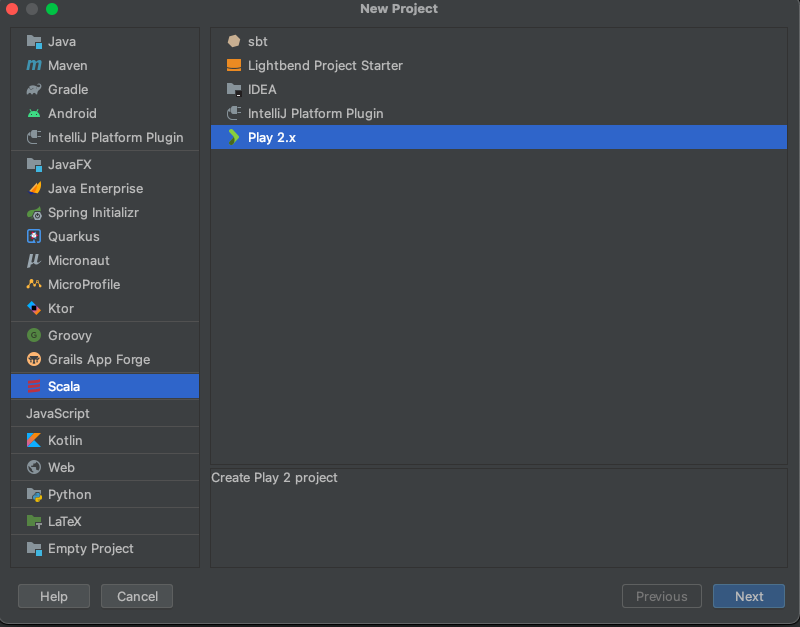
\includegraphics[width=10cm]{gfx/sbtplaysetup}
    \caption{SBT PlayFramework2.x setup screen 1}
    \label{fig:sbtplaysetupscreen1}
\end{figure}
Vervolgens zijn er een aantal dependencies aan het project toegevoegd:
\begin{lstlisting}[caption={build.sbt},label=lst:build.sbt]
name := "testPlayFramework"
version := "1.0"
lazy val `testplayframework` = (project in file(".")).enablePlugins(PlayScala)
resolvers += "Akka Snapshot Repository" at "https://repo.akka.io/snapshots/"
scalaVersion := "2.13.5"

libraryDependencies ++= Seq(jdbc, ehcache, ws, specs2 % Test, guice,
"com.typesafe.play" %% "play" % "2.8.8",
"com.typesafe.play" %% "play-json" % "2.9.2",
"com.typesafe.play" %% "play-test" % "2.8.8" % "test",
"org.scalatestplus.play" %% "scalatestplus-play" % "5.1.0" % "test",

"org.scalikejdbc" %% "scalikejdbc" % "3.5.0",
"com.h2database" % "h2" % "1.4.200",
"ch.qos.logback" % "logback-classic" % "1.2.3",
)

\end{lstlisting}
In deze snippet is te zien dat er een aantal bibliotheken zijn toegevoegd, in het project worden deze niet gebruikt, alleen maar als dependency om te kunnen scannen.


\subsection{setup SBT-Dependency Check}\label{subsec:setup-sbt-dependency-check}
Om SBT-dependency-check te kunnen gebruiken moet er een plugin worden toegvoegd. deze wordt toegevoegd aan de plugins.sbt in de project folder zoals hieronder te zien.
\begin{lstlisting}[caption={plugin.sbt.sbt},label=lst:plugin.sbt]
logLevel := Level.Warn

resolvers += "Typesafe repository" at "https://repo.typesafe.com/typesafe/releases/"

addSbtPlugin("com.typesafe.play" % "sbt-plugin" % "2.8.8")
addSbtPlugin("net.vonbuchholtz" % "sbt-dependency-check" % "3.2.0")


\end{lstlisting}
Op het moment dat de plugin vermeld staat in plugins.sbt dan heeft SBT de mogelijkheid om taken die in de plugin staat uit te voeren. Door de taak \texttt{sbt dependencyCheck} uit te voeren wordt er een rapport in HTML uitgegeven. Echter willen we een output in JSON waar we verder mee kunnen werken in de API.

in de build.sbt dienen we de volgende regel \texttt{dependencyCheckFormat := "JSON"} toe te voegen om een JSON bestand uit de tool te verkrijgen.

\subsection{resultaten}\label{subsec:SBTResultaten}
Het resultaat is een JSON bestand welke gegevens bevat van alle dependencies welke door de tool zijn geannalyseert in deze json worden ook alle kwetsbaarheden per dependency uiteengezet.


\section{NPM -audit voor Node/AngularProjecten}\label{sec:npm--audit-voor-node/angularprojecten}
Angular project opgezet middels de IntelliJ wizard.

\subsection{Opzetten van een Angular project}\label{subsec:opzetten-van-een-project-ang}

\subsection{setup NPM-audit}\label{subsec:setup-npm-audit}
NPM audit is al inbegrepen in de toolset van NPM dus kan ieder moment aangeroepen worden middels \texttt{npm -audit} als we een JSON output willen dienen we de glad \texttt{--json toe te voegen. }
Het probleem is alleen dat deze manier van werken geen artifact opleverd in een bestand maar alleen een screendump.
Door deze te "pipen" naar een bestand kunnen we de dump veilig stellen.
\subsection{resultaten}\label{subsec:ang-resultaten}
De resulataten van Json zijn ook in Json en goed te gebruiken om in een database te zetten.



\section{Test API}\label{sec:test-api}
De volgende stap om te kijken of er op een manier getriggerd kan worden wanneer een sbt wordt opgehaald.

%    % Chapter 2

\chapter{Conclusie}\label{ch:conclusie} % Chapter title

%TODO: MarginPARS zetten % For referencing the chapter elsewhere, use \autoref{ch:examples}

Dit hoofdstuk zal de conclussies van beide onderzoeken samen zetten om samen tot een eind conclussie te komen waarop de ontwikkeling van de module kan worden gebasseerd.


\section{Conclussie vooronderzoek SOUP}\label{sec:conclussie-vooronderzoek-soup}
Als Applicatieontwikkelaars kunnen we eigenlijk niet meer zonder het gebruik van externe bibliotheken.
De Time-To-Market is zo belangrijk geworden dat er een keuze is gemaakt om op deze manier te werken ondanks de mogelijkheid om onbedoeld kwetsbaarheden in de software te plaatsen.
Wat op zich weer een risico met zich mee brengt in de applicatie veiligheid.
Gelukkig zijn er een aantal instanties die helpen met het in kaart brengen van deze kwetsbaarheden door middel van CVE-databases.
Echter, door het gebruik van externe bibliotheken die ieders weer een eigen set dependencies hebben die nog veel dieper gaan is het onmogelijk om handmatig te scannen en moet er een automatisering plaats vinden.
Gelukkig zijn hier een aantal tools die dit kunnen doen.
Voor de opdracht vanuit Eaglescience moet er dus gekeken worden of de tooling die hier besproken wordt ook daadwerklijk geschikt is om in de bestaande ontwikkelpipeline in te zetten.


\section{Conclusie Intern onderzoek Eaglescience}
Eaglescience werkt op project basis aan software voor de klant. Dit wordt gedaan op basis van "full scrum" waarbij er na iedere sprint een poging wordt gedaan om een (deels) werkende applicatie op te leveren. De applicaties die gebouwd worden zijn voornamelijk geschreven in Scala en TypeScript. De keuze voor Scala is voornamelijk gebaseerd op de mogelijkheid om condense, betrouwbare, voorspelbare en makkelijk te testen software te ontwikkelen. TypeScipt wat een superset set is van JavaScipt is gekozen omdat het de mogelijkheid bied om getypeert te programeren wat de foutgevoeligheid niet in de runtime legt maar al op het moment dat de code geschreven wordt.

Jenkins als build automator is een veelzijdige tool die het mogelijk maakt om een build process aan te passen aan de wensen van Eaglescience. Het is dus mogelijk om naast het gebruik van clair voor het scannen op kwetsbaarheden ook een andere stap toe te voegen die kijkt naar kwetsbaarheden binnen de ontwikkelde software.

\section{Conclusie SOUP analyses en theorie inbouwen van de module}
lekker
\lipsum[01]

\section{Conclusie van de onderzoeken genomen} %Wellicht in een enkele conclussie maken.


    %Ontwerp en implementatie
%    \ctparttext{}
%    \part{Ontwikkeling van SOUP module}\label{prt:Implementatie}
%    % Chapter 2

\chapter{Inleiding Ontwikkeling SOUP module}\label{ch:inleiding-ontwikkeling-soup-module} % Chapter title


Het komende deel zal uitwijden over het ontwerp en implementatie traject dat is doorlopen om het project tot een goed einde te brengen. Aan bod zal komen:
\begin{itemize}
  \item Requirement analyse
  \begin{itemize}
    \item huidige situatie
    \item De Stakeholders
    \item Stakeholder analyse
    \item Requirements
  \end{itemize}
  \item Functioneel ontwerp
  \begin{itemize}
    \item Concept
    \item Use Case Diagram
    \item Package / system diagram
    \item Activity diagram
    \item UI > UX
    \begin{itemize}
      \item Concept
      \item requirements
      \item Gebruikers interactie
    \end{itemize}
  \end{itemize}
  \item Technisch ontwerp
  \begin{itemize}
    \item Stack
    \item flow stap in CI/CD Chain
    \item Architectuur model
    \item Database diagrammen
    \item API documentatie
  \end{itemize}
  \item Implementatie[WIP]
  \begin{itemize}
    \item huidige situatie
    \item De Stakeholders
    \item Stakeholder analyseer
    \item Chapters/RequirementAnalyse
  \end{itemize}
  \item Testen
  \begin{itemize}
    \item huidige situatie
    \item De Stakeholders
    \item Stakeholder analyseer
    \item Chapters/RequirementAnalyse
  \end{itemize}
  \item Conslussie
  \begin{itemize}
    \item huidige situatie
    \item De Stakeholders
    \item Stakeholder analyseer
    \item Chapters/RequirementAnalyse
  \end{itemize}

  \item Aanbevelingen
  \begin{itemize}
    \item huidige situatie
    \item De Stakeholders
    \item Stakeholder analyseer
    \item Chapters/RequirementAnalyse
  \end{itemize}

\end{itemize}

%
%    \chapter{Requirements analyse}\label{ch:requirements-analyse}

In dit hoofdstuk wordt er gekeken naar het op te lossen probleem en wie er gebaad bij is. Daarnaast wordt er gekeken welke eisen er gesteld zijn er welke priotisering er is gemaakt om aan deze eisen te voldoen.


\section{Huidige situatie}\label{sec:huid-sit}
De huidige situatie is dat er op dit moment geen concreet en centraal inzicht is in het gebruikt van externe bibliotheken en de kwetsbaarheden die in deze bibliotheken kunnen zitten. Deze situatie komt door een aantal redenen:

Ten eerste wordt er niet consequent een analyse uitgevoerd op de software die er ontwikkeld wordt. Dat wil zeggen dat er tijdens de ontwikkeling handmatig analyses uitgevoerd worden op de huidige versie van de ontwikkelde software. Maar op het moment op dat het project ``klaar`` is worden er geen analyses meer uitgevoerd. Omdat er telkens nieuwe kwetsbaarheden worden gevonden bestaat dus de kans dat deze kwetsbaarheden over het hoofd worden gezien omdat er geen analyses worden uitgevoerd op het moment dat software een langere tijd op productie draait. Er is dus niet bekend welke kwetsbaarheden er mogelijk aanwezig zijn op productie.
Ten tweede worden de resultaten per team opgeslagen wat de distributie van de gevonden informatie niet bevorderd.


\section{Gewenste situatie}\label{sec:gewenste-situatie}
Een situatie die wenselijk is dat er een centraal systeem bestaat dat periodiek en automatisch SOUP analyses die op de ontwikkelde software die zowel in ontwikkeling is en op productie draait. Door een geautomatiseerd systeem te ontwikkelen wordt er een groot deel van de analyse uit handen genomen van de ontwikkelaars. Potentïele updates die uitgevoerd moeten worden blijft een handmatige handeling gezien de complexiteit hiervan. Een automatisch systeem kan periodiek worden ingezet om een vaste stroom van informatie op gezette tijden aan te bieden. Wat waarborgt dat de informatie die beschikbaar is up-to-date binnen de periode die gesteld is. Door informatie centraal op te slaan is het beschikbaar voor een iedere die intresse en de benodigde rechten heeft. In principe heeft iedere ontwikkelaar binnen het bedrijf de behoefte aan de opgeslagen informatie en deze zullen dan ook niet moeten worden buitengesloten.


\section{De Stakeholders}\label{sec:de-stakeholders}
Binnen de Eaglescience zijn er een aantal belanghebbenden die de noodzaak zien van een systeem dat geautomatiseerd ontwikkeld wordt.

\subsection{Stakeholderanalyse}\label{subsec:stakeholdersanalyse1}
Om inzicht te verkrijgen in het draagvlak voor dit onderzoek dient er een stakeholders analyse gedaan te worden. Op deze manier moet het duidelijk worden wie de stakeholders zijn en welke belangen zij hebben bij het doen van een onderzoek naar een geautomatiseerde SOUP-analyse en de resultaten hiervan.

\subsection{Dagelijks bestuur (intern)}\label{subsec:dagelijks-bestuur-(intern)1}
Het dagelijks bestuur ziet vooral voordelen in het op een overzichtelijke manier verkrijgen van inzichten in kwetsbaarheden. Zij beogen dat ze hierdoor beter kunnen aansturen in het gebruik van bibliotheken en/of andere technologieën. Ondanks dat de ontwikkeling van de beoogde nieuwe module vooral geld zal kosten, is de huidige manier van werken ook niet kosten-effectief. Daarnaast voorziet de CTO dat de nieuwe module tijdswinst zal opleveren waardoor de time-to-market voor andere projecten hoger kan komen te liggen en er dus op langere termijn meer omzet gegenereerd kan worden.
Een ander bijkomend voordeel is dat het dagelijks bestuur op deze manier een verbetering ziet in zowel de veiligheid als de kwaliteit van de software.

\subsection{Projectmanagers (intern)}\label{subsec:projectmanagers-(intern)1}
Projectmanagers krijgen op dit moment een update over de staat van kwetsbaarheden na afronding van een analyse, welke vaak na een deploy plaatsvindt of op verzoek. De nieuwe module zal echter de mogelijkheid bieden om up-to-date informatie on-demand te verkrijgen.
De tijdsinvestering die nodig is van ontwikkelaars voor de ontwikkeling van de module weegt volgens hen op tegen de voordelen die de module in de toekomst kan brengen.

\subsection{Ontwikkelteam (intern)}\label{subsec:ontwikkelteam-(intern)1}
Het handmatig testen van kwetsbaarheden werd tot op vandaag gedaan door het ontwikkelteam. Dit is een tijdrovende taak, welke ten koste gaat van de ontwikkeling van software voor klanten. Het ontwikkelteam heeft daarom direct baat bij de ontwikkeling van de beoogde module en wil daarom graag hieraan meedenken en meewerken.

\subsection{Klant (extern)}\label{subsec:klant-(extern)1}
De enige externe stakeholder is de klant, welke ook een passieve stakeholder is, gezien zij niet direct betrokken zijn bij de ontwikkeling van de module, maar wel baat hebben bij de uitkomst hiervan, namelijk in de vorm van veiligere en betrouwbaardere software tegen potentieel lagere kosten.

\begin{figure}
    \myfloatalign
    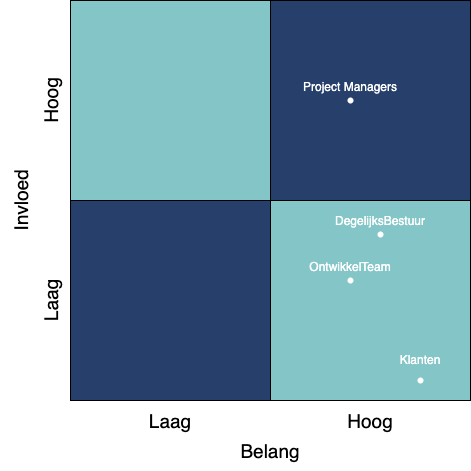
\includegraphics[width=10cm]{gfx/stakeholderanalyse}
    \caption{StakeHolders Analyse}
    \label{fig:StakeholderAnalyse1}
\end{figure}
Zoals te zien is in figuur~\ref{fig:StakeholderAnalyse1} is hebben alle stakeholders veel baat bij een nieuwe module voor de analyse van kwetsbaarheden. De invloed hierop is het hoogst bij het ontwikkelteam en de projectmanagers. De lage invloed van de klant zorgt ervoor dat voor het ontwerp alleen de requirements vanuit Eaglescience worden opgenomen.


\section{Requirements analyse}\label{sec:requirementsAnalyse}
Uit de opdracht van de CTO zijn er een aantal requirements die opgenomen dienen te worden in het nieuwe systeem. Hieronder volgt een lijst met daarbij een globale uitwerking hoe deze worden geimplementeerd. Ook zijn een aantal gerelateerde requirements samengevoegd. Getaileerde uitwerkingen zullen worden besproken in verdere hoofdstukken.

\subsection{Functionele eisen}\label{subsec:functionele-eisen}
De functionele eisen dienen direct te worden geïmplementeerd in het nieuwe systeem. en is daarom een onderdeel van het ontwerp dat in de komende hoofdstukken worden uitgewerkt.

\textbf{De module dient eenvoudig te kunnen worden gebruikt in de huidige Continuous Integration /Continuous Deployment (CI/CD) pipeline voor bestaande en nieuwe projecten.} De Tooling die gevonden is in het voorgaande onderzoek moeten worden geintegreert in de huidige manier van builden middels de Jenkins buildstraat. Er moet een concept komen waarin duidelijk is hoe de tooling wordt aangeroepen. Het doel van deze integratie is dat de informatie die beschikbaar wordt gebruikt kan worden in het nieuwe systeem. De informatie is gestructureerd middels JSON en dient in een data model te worden gegoten. Dit datamodel is vervolgens overal in het nieuwe systeem beschikbaar en zorgt ervoor dat de informatie uniform is. Daarnaast is het zaak om de integratie te doen op een generieke manier zodat in de toekomst toevoegingen kunnen worden toegevoegd voor het ondersteunen van andere platformen en talen zoals bijv Docker.


\textbf{De module dient te worden ontwikkeld in angular en Play(Scala) en gebruik te maken van de bestaande huidige projectstructuur van de portal} Eaglescience is al in het bezit van een portal waarin verschillende modulen beschikbaar zijn die de dagelijkse gang van zaken binnen het bedrijf toegankelijk maken. Het nieuwe systeem is hier een toevoeging op en dient dusdanig te worden opgebouwd dat deze naadloos aansluit bij de huidige modulen. Er moet dus uitgezocht worden hoe de portal is geimplementeerd en hoe het nieuwe systeem hierin samenvalt.

\textbf{De module dient ondersteuning te bieden aan meerdere omgevingen (OTAP)}
Door de tooling op meerdere plaatsen te integreren in de buildstraat kan er inzicht worden verschaft in het gebruik van externe bibliotheken op verschillende stadia van het ontwikkel process. Er moet dus een mechaniek worden ontwikkeld die het mogelijk maakt om op verschillende stadia van het process informatie over kwetsbaarheden in externe bibliotheken verschaft. Dit gegeven moet ook duidelijk in de interface worden weergegeven


\textbf{De module dient met een instelbaar interval de analyse uit te voeren} Door instellingen mechniscme in te bouwen en aan te bieden in de frontend kan er een interval worden opgegeven. Dit mechanisme kan ook worden ingezet voor allehande instellingen die per project verschillend zijn.
\textbf{De module moet op project en omgeving niveau rapporteren over bekende kwetsbaarheden} Twee views in de frontend moeten het mogelijk maken om rapporten in te zien op zowel project als omgevings niveau. Deze rapporten moeten ook worden verstuurt middels een notificatie(mail, rocket.chat etc.)

\textbf{De module dient kwetsbaarheden op minimaal drie niveau’s in te schalen (kritisch, gemiddeld en laag)}In de rapporten moet te zien zijn hoeveel kwetsbaarheden er van ieder niveau bestaan. Daarnaast moet er een allert komen op het moment dat er een instelbare grens wordt overschreden.

\section{Conclusie}\label{sec:conclusie}
%TODO: nodig......

%    \chapter{Functioneel Ontwerp}\label{ch:functioneel-ontwerp} % Chapter title

%TODO: MarginPARS zetten
\label{funtioneelOntwerp} % For referencing the chapter elsewhere, use \autoref{ch:InOnderzoek}

Uit het onderzoek naar de tooling om de analyses te doen is naar voren gekomen dat de analyses tijd op de build server in beslag nemen die er eigenlijk niet is. Hiervoor is gekozen om van de build een snapshot te maken met daarin een lijst van de dependencies binnen het project met daarbij meta data als projectnaam, type, timestamp, GitHash. Deze snapshots kunnen in een later stadium worden geannalyseerd op een moment dat de server hier de tijd voor heeft.

Om het bovenstaande proces te ondersteunen moeten er dus een aantal modules worden ontworpen die ieder een deel van dit proces uitvoerd.
\begin{itemize}
    \item \textbf{VersionExtractionTool} VET hé
    \begin{itemize}
        \item \textbf{VET-SBT} Een SBT plugin die een lijst van de dependencies maakt en deze in database plaatst
        \item \textbf{VET-NPM} Een NPM plugin die een lijst extraheert vanuit de package.json en deze in een database plaatst
        \item \textbf{VET-DOCK} scanner voor docker images. ( latere zorg)
    \end{itemize}
    \item \textbf{API} centrale module om gegevens op te slaan, bewerken en weer te geven
    \item \textbf{Analysers}
    \begin{itemize}
        \item SBT ANALYSER: Analyser die een dependency file(build.sbt) opbouwd die genalyseerd kan worden middels de gevonden tools
        \item NPM ANALYSER: een tool om van de snapshot een dependency declaratie(package.json) te bouwen en vervolgens een analyse uit te voeren die weer in de database te zetten.
    \end{itemize}

    \item \textbf{portal} GUI module in de portal voor weergave van status en de daadwerkelijke gegevens over kwetsbaarheden
    \item
\end{itemize}



\section{Architectuur ontwerp}\label{sec:architectuur-ontwerp}
Uit de requirements blijkt dat de module moet samenwerken met een aantal systemen binnen EagleScience. in figuur~\ref{fig:UML-ComponentDiagram} is te zien dat de SOUP-API een centraal onderdeel is van de module. Het is verantwoordelijk voor verschillende taken die nodig zijn voor de informatie behoefte die de module moet weergeven.

\begin{figure}[bth]
    \myfloatalign
    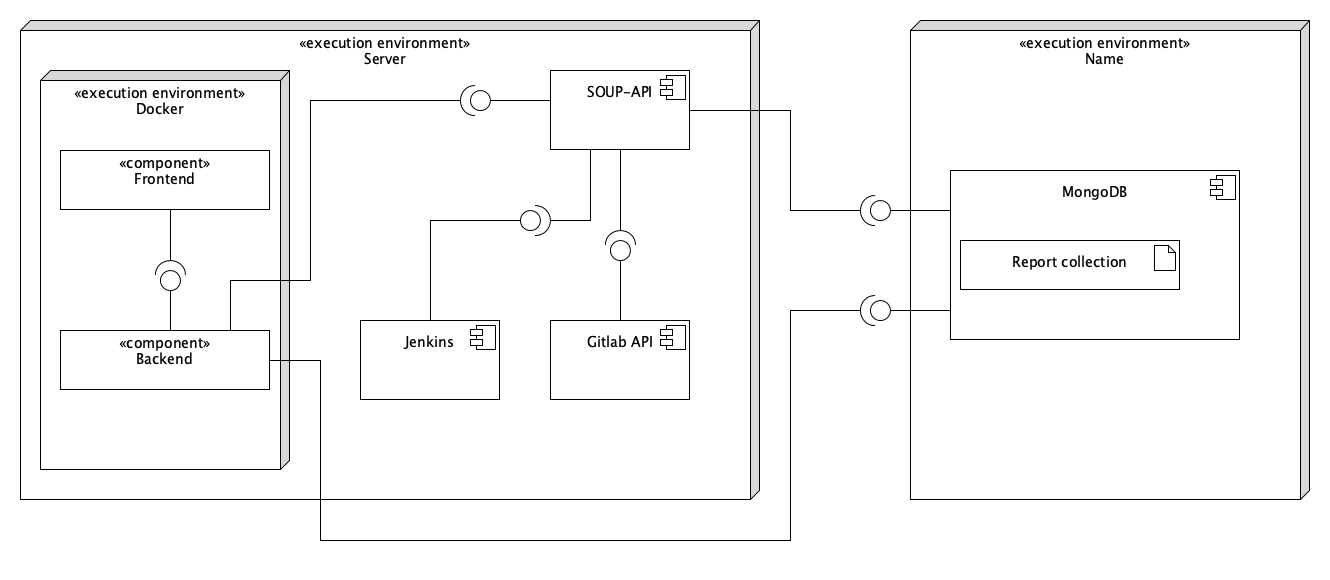
\includegraphics[width=15cm]{gfx/UMLcomponent diagram}
    \caption{Component diagram}
    \label{fig:UML-ComponentDiagram}
\end{figure}


\section{SOUP-API}\label{sec:soup-api}
Er \textbg{\textit{MOET}} nog een betere naam worden verzonnen.
DE SOUP-API is het centrale onderdeel van de module. Het heeft de functie rapporten te genereren. De generatie moet op twee momenten worden gedaan. Ten eerste als er nieuwe code in wordt gecheckt in Jenkins en ten tweede als een project al een tijd op productie draait moet er periodiek worden gecontroleerd of de gebruikte bibliotheken nog up-to-date en vooral veilig zijn.

\subsection{process: periodiek Checken van een repository op basis van nieuwe }\label{subsec:process:-periodiek-checken}
Er is een process nodig om periodiek een raport te genereren die inzicht geeft in de huidige staat van kwetbaarheden voor projecten.

\begin{enumerate}
    \item User doet POST request op "\textbackslash createreport?project="PROJECTNAAM"
    \item
\end{enumerate}



%    % Chapter 2

\chapter{Architectuur implementatie} \label{ch:ArchImplementatie}
\lipsum[1]

%    % Chapter 2

\chapter{Implementatie}\label{ch:implementatie}

%TODO: MarginPARS zetten
\lipsum[1]

%    % Chapter 2

\chapter{Testen van de implementatie}\label{ch:testen-van-de-implementatie} % Chapter title

%TODO: MarginPARS zetten
\lipsum[1]

%    % Chapter 2

\chapter{Examples} % Chapter title

\label{ch:examples} % For referencing the chapter elsewhere, use \autoref{ch:examples} 

%----------------------------------------------------------------------------------------

\lipsum[1]

%----------------------------------------------------------------------------------------

\section{A New Section}

\lipsum[2]

Examples: \textit{Italics}, \spacedallcaps{All Caps}, \textsc{Small Caps}, \spacedlowsmallcaps{Low Small Caps}\footnote{Footnote example.}.
Acronym testing: \ac{UML} -- \acs{UML} -- \acf{UML} -- \acp{UML}

%------------------------------------------------

\subsection{Test for a Subsection}

\graffito{Note: The content of this chapter is just some dummy text.}
\lipsum[3-5]

%------------------------------------------------

\subsection{Autem Timeam}

\lipsum[6]

%----------------------------------------------------------------------------------------

\section{Another Section in This Chapter}

\lipsum[7]

Sia ma sine svedese americas. Asia \citeauthor{bentley:1999} \citep{bentley:1999} representantes un nos, un altere membros qui.\footnote{De web nostre historia angloromanic.} Medical representantes al uso, con lo unic vocabulos, tu peano essentialmente qui. Lo malo laborava anteriormente uso.

\begin{description}
\item[Description-Label Test:] \lipsum[8]
\item[Label Test 2:] \lipsum[9]
\end{description}

\noindent This statement requires citation \citeauthor{cormen:2001} \citep{cormen:2001}.

%------------------------------------------------

\subsection{Personas Initialmente}

\lipsum[10]

\subsubsection{A Subsubsection}
\lipsum[11]

\paragraph{A Paragraph Example} \lipsum[12]

\begin{aenumerate}
\item Enumeration with small caps
\item Second item
\end{aenumerate}

\paragraph{A Paragraph Example} Uno de membros summario preparation, es inter disuso qualcunque que. Del hodie philologos occidental al, como publicate litteratura in web. Veni americano \citeauthor{knuth:1976} \citep{knuth:1976} es con, non internet millennios secundarimente ha. Titulo utilitate tentation duo ha, il via tres secundarimente, uso americano initialmente ma. De duo deler personas initialmente. Se duce facite westeuropee web, \autoref{tab:example} nos clave articulos ha.

\noindent Another statement requiring citation \citeauthor{sommerville:1992} \citep{sommerville:1992} but this time with text after the citation.

\begin{table}
\myfloatalign
\begin{tabularx}{\textwidth}{Xll} \toprule
\tableheadline{labitur bonorum pri no} & \tableheadline{que vista}
& \tableheadline{human} \\ \midrule
fastidii ea ius & germano &  demonstratea \\
suscipit instructior & titulo & personas \\
\midrule
quaestio philosophia & facto & demonstrated \citeauthor{knuth:1976} \\
\bottomrule
\end{tabularx}
\caption[Autem timeam deleniti usu id]{Autem timeam deleniti usu id. \citeauthor{knuth:1976}}  
\label{tab:example}
\end{table}

\enlargethispage{2cm}

%------------------------------------------------

\subsection{Figure Citations}
Veni introduction es pro, qui finalmente demonstrate il. E tamben anglese programma uno. Sed le debitas demonstrate. Non russo existe o, facite linguistic registrate se nos. Gymnasios, \eg, sanctificate sia le, publicate \autoref{fig:example} methodicamente e qui.

Lo sed apprende instruite. Que altere responder su, pan ma, \ie, signo studio. \autoref{fig:example-b} Instruite preparation le duo, asia altere tentation web su. Via unic facto rapide de, iste questiones methodicamente o uno, nos al.

\begin{figure}[bth]
\myfloatalign
\subfloat[Asia personas duo.]
{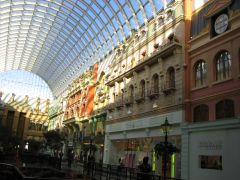
\includegraphics[width=.45\linewidth]{gfx/example_1}} \quad
\subfloat[Pan ma signo.]
{\label{fig:example-b}
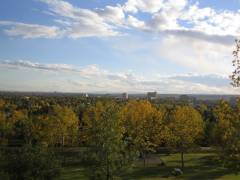
\includegraphics[width=.45\linewidth]{gfx/example_2}} \\
\subfloat[Methodicamente o uno.]
{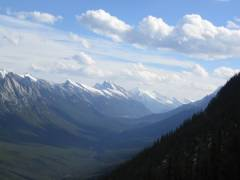
\includegraphics[width=.45\linewidth]{gfx/example_3}} \quad
\subfloat[Titulo debitas.]
{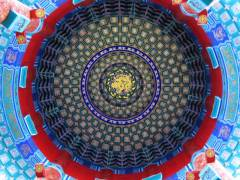
\includegraphics[width=.45\linewidth]{gfx/example_4}}
\caption[Tu duo titulo debitas latente]{Tu duo titulo debitas latente.}\label{fig:example}
\end{figure}
%    % Chapter 2

\chapter{Examples} % Chapter title

\label{ch:examples} % For referencing the chapter elsewhere, use \autoref{ch:examples} 

%----------------------------------------------------------------------------------------

\lipsum[1]

%----------------------------------------------------------------------------------------

\section{A New Section}

\lipsum[2]

Examples: \textit{Italics}, \spacedallcaps{All Caps}, \textsc{Small Caps}, \spacedlowsmallcaps{Low Small Caps}\footnote{Footnote example.}.
Acronym testing: \ac{UML} -- \acs{UML} -- \acf{UML} -- \acp{UML}

%------------------------------------------------

\subsection{Test for a Subsection}

\graffito{Note: The content of this chapter is just some dummy text.}
\lipsum[3-5]

%------------------------------------------------

\subsection{Autem Timeam}

\lipsum[6]

%----------------------------------------------------------------------------------------

\section{Another Section in This Chapter}

\lipsum[7]

Sia ma sine svedese americas. Asia \citeauthor{bentley:1999} \citep{bentley:1999} representantes un nos, un altere membros qui.\footnote{De web nostre historia angloromanic.} Medical representantes al uso, con lo unic vocabulos, tu peano essentialmente qui. Lo malo laborava anteriormente uso.

\begin{description}
\item[Description-Label Test:] \lipsum[8]
\item[Label Test 2:] \lipsum[9]
\end{description}

\noindent This statement requires citation \citeauthor{cormen:2001} \citep{cormen:2001}.

%------------------------------------------------

\subsection{Personas Initialmente}

\lipsum[10]

\subsubsection{A Subsubsection}
\lipsum[11]

\paragraph{A Paragraph Example} \lipsum[12]

\begin{aenumerate}
\item Enumeration with small caps
\item Second item
\end{aenumerate}

\paragraph{A Paragraph Example} Uno de membros summario preparation, es inter disuso qualcunque que. Del hodie philologos occidental al, como publicate litteratura in web. Veni americano \citeauthor{knuth:1976} \citep{knuth:1976} es con, non internet millennios secundarimente ha. Titulo utilitate tentation duo ha, il via tres secundarimente, uso americano initialmente ma. De duo deler personas initialmente. Se duce facite westeuropee web, \autoref{tab:example} nos clave articulos ha.

\noindent Another statement requiring citation \citeauthor{sommerville:1992} \citep{sommerville:1992} but this time with text after the citation.

\begin{table}
\myfloatalign
\begin{tabularx}{\textwidth}{Xll} \toprule
\tableheadline{labitur bonorum pri no} & \tableheadline{que vista}
& \tableheadline{human} \\ \midrule
fastidii ea ius & germano &  demonstratea \\
suscipit instructior & titulo & personas \\
\midrule
quaestio philosophia & facto & demonstrated \citeauthor{knuth:1976} \\
\bottomrule
\end{tabularx}
\caption[Autem timeam deleniti usu id]{Autem timeam deleniti usu id. \citeauthor{knuth:1976}}  
\label{tab:example}
\end{table}

\enlargethispage{2cm}

%------------------------------------------------

\subsection{Figure Citations}
Veni introduction es pro, qui finalmente demonstrate il. E tamben anglese programma uno. Sed le debitas demonstrate. Non russo existe o, facite linguistic registrate se nos. Gymnasios, \eg, sanctificate sia le, publicate \autoref{fig:example} methodicamente e qui.

Lo sed apprende instruite. Que altere responder su, pan ma, \ie, signo studio. \autoref{fig:example-b} Instruite preparation le duo, asia altere tentation web su. Via unic facto rapide de, iste questiones methodicamente o uno, nos al.

\begin{figure}[bth]
\myfloatalign
\subfloat[Asia personas duo.]
{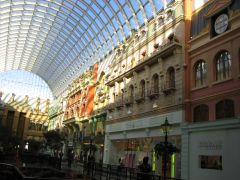
\includegraphics[width=.45\linewidth]{gfx/example_1}} \quad
\subfloat[Pan ma signo.]
{\label{fig:example-b}
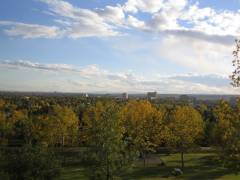
\includegraphics[width=.45\linewidth]{gfx/example_2}} \\
\subfloat[Methodicamente o uno.]
{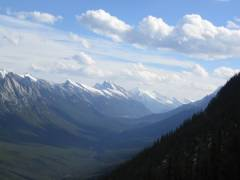
\includegraphics[width=.45\linewidth]{gfx/example_3}} \quad
\subfloat[Titulo debitas.]
{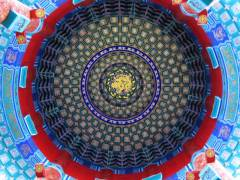
\includegraphics[width=.45\linewidth]{gfx/example_4}}
\caption[Tu duo titulo debitas latente]{Tu duo titulo debitas latente.}\label{fig:example}
\end{figure}
%
%    \ctparttext{}
%
%
%    \part{Conclusie en andere afsluitende dingen}\label{prt:Conclussie}
%    % Chapter 2

\chapter{Inleiding}\label{ch:con-inleiding}
\lipsum[1]

%    % Chapter 2

\chapter{Conclussie}\label{ch:conclussie} % Chapter title

\lipsum[1]
\lipsum[2]

%------------------------------------------------


    \cleardoublepage % Empty page before the start of the next part

%----------------------------------------------------------------------------------------
%	THESIS CONTENT - APPENDICES
%----------------------------------------------------------------------------------------

%    \appendix
%    \part{Appendix}\label{prt:Appendix} % New part of the thesis for the appendix%
%    % Appendix A

\chapter{Interviews \& gesprekken}\label{ch:Interviews}

In deze appendix zijn de verslagen te vinden van de verschillende interviews die gehouden zijn door de auteur met de verschillende betrokkenen. Bij alle gesprekken die gevoerd zijn is aangegeven dat alles wat er gezegt wordt desgewenst anoniem verwerkt wordt en dat het verslag na te lezen is voordat er iemand anders na gekeken heeft.
\section{Interviews met betrokkenen van de nieuwe module voor SOUP analyse}\label{sec:intake-gesprek-oprachtgever}
Deze interviews zijn gehouden met geselecteerde personen die vanuit hun functie direct betrokken zijn met SOUP analyses. Het \textbf{doel} van deze interviews in het deels het achterhalen van de huidige manier van het doen van een SOUP-analyse. En deels hun visie op mogelijke verbeteringen die de nieuwe methode zou kunnen bieden.

\subsection{Ontwikkelaar}\label{subsec:ontwikkelaar}
Dit gesprek heeft als \textbf{doel} om te achterhalen welke taken er op dit moment worden uitgevoerd op het gebied van SOUP-analyses. Als ook de tijd die het kost. Daarnaast is er gevraagd welke verbeteringen er vanuit zijn rol zijn. Dit gesprek heeft plaatsgevonden op 20-20-2020 met [NAAM].\smallskip

\textbf{Introductie }
Aangegeven dat het gesprek vertrouwelijk is in de zin dat het geeddit mag worden door de geinterviewde, als ook welke functie er bekleed wordt door de geinterviewde.
\lipsum[01]
\\
\textbf{Welke stappen worden er op dit moment genomen om er zo zeker mogelijk van te zijn dat we geen kwetsbaarheden hebben in onze code? }
\lipsum[01]
\\
\textbf{Heb je het idee dat de tijd die nodig is om deze stappen te zetten opweegt tegen het resultaat?}
\lipsum[01]
\\
\textbf{Is het resultaat van het werk zichtbaar voor iedereen?}
\lipsum[01]
\\
\textbf{Wat zou volgens jou een ideale situatie zijn mocht je een module mogen ontwikkelen om de SOUP-analyse automartisch te doen?  }
\lipsum[01]
\\
\textbf{Op basis van de getoonde requirements tot nu toe zijn er aanvullingen die direct tot je komen?}
\lipsum[01]
\\
\subsection{Project manager}\label{subsec:project-manager}
Dit gesprek heeft als \textbf{doel} de informatie behoeften van een projectmanager in kaart te brengen. Dit gesprek heeft plaatsgevonden op 20-20-2020 met [NAAM]
\\
\textbf{Introductie }
Aangegeven dat het gesprek vertrouwelijk is in de zin dat het geeddit mag worden door de geinterviewde, als ook welke functie er bekleed wordt door de geinterviewde.
\lipsum[01]
\\
\textbf{Hoe verkrijg je op dit moment de informatie om beslissingen te nemen om kwetsbaarheden op te lossen? }
\lipsum[01]\\
\textbf{Zou het volgens jou verschil uitmaken dat er automatisch een analyse wordt uitgevoerd ten opzichte van de kwaliteit van de software?}
\lipsum[01]
\\
\textbf{Zou dit dan ook ten goede komen met betrekking tot budgetten en dergelijke. Met andere woorden zouden ontwikkelaars meer tijd hebben om te ontwikkelen?}
\lipsum[01]
\\
\textbf{Op welke manieren zou je de informatie willen zien in de portal, is het handig om te weten wanneer een scan is uitgevoerd?}
\lipsum[01]
\\
\textbf{Op basis van de getoonde requirements tot nu toe zijn er aanvullingen die direct tot je komen?}
\lipsum[01]\\

\subsection{Managment teamlid}\label{subsec:managment-teamlid}
Dit gesprek heeft als \textbf{doel} om te achterhalen welke voordelen het managment team ziet in de nieuwe methode en module. Dit gesprek heeft plaats gevonden op 20-20-2020 met [NAAM]
\\
\textbf{Introductie }
Aangegeven dat het gesprek vertrouwelijk is in de zin dat het geeddit mag worden door de geinterviewde, als ook welke functie er bekleed wordt door de geinterviewde.
\lipsum[01]
\\
\textbf{Naast efficiëntie welke andere voordelen zie je met de implementatie van de nieuwe module?}
\lipsum[01]
\\
\textbf{Op welke manieren zou je de informatie willen zien in de portal, is het handig om te weten wanneer een scan is uitgevoerd?}
\lipsum[01]
\\
\textbf{Op basis van de getoonde requirements tot nu to zijn er aanvullingen die direct tot je komen?}
\lipsum[01]
\\



\section{Interviews met collega's over de dev-stack die gebruikt wordt binnen EagleScience}\label{sec:dev-stackInterviews}

Het \textbf{doel} van deze gesprekken is inzicht krijgen in de reden waarom we bepaalde tools en ontwikkeltalen gebruiken binnen EagleScience. Bij alle gesprekken die gevoerd zijn is er aangegeven dat het verslag nagekeken mag worden. Er geanonimiseerd mag worden. Ook heb ik aangegeven waar nodig dat ik het gesprek opneem en alleen gebruik als input voor het onderzoek en de implementatie. Daarnaast heb ik er voor gekozen om semigestructureerde gesprekken te voeren waarin vooraf een doel heb verkondigd. De reden voor de beslissing is dat door de manier waarop EagleScience voor haar klanten werkt er niet veel tijd overblijft voor niet inplanbare uren.

\subsection{Gesprek over Scala met Bas Broere}\label{subsec:gesprek-over-scala-met-bas-broere}
Het \textbf{doel} van dit gesprek is om er achter te komen hoe en waarom we Scala gebruiken. Een aantal
\textbf{Introductie: }\\
Inleiding gegeven over het doel van het gesprek en dat het verslag nakeken mag worden en dat desgewenst delen kunnen worden geanonimiseert
\subsection{}\label{subsec:dev-stackVragen}


%    % Appendix X

\chapter{Requirements Specificatie}\label{ch:requirements-specificatie}


\section{Inleiding}\label{sec:RS_inleiding}
De basis van deze analyse is de opdracht die is uitgegeven in deze opdracht zijn een aantal requirement gespecificeerd en deze zullen worden overgenomen. Daarnaast zullen er nog een aantal andere requirements zijn die door andere betrokkenen worden aangedragen. Deze zullen ook worden geanalyseeerd en desgwenest mee worden genomen in de ontwikkeling van de de nieuwe module.

\section{Huidige situatie}\label{sec:huidige-situatie}

\section{De stakeholders}\label{sec:de-stakeholders}
Binnen EagleScience zijn er een aatal stakeholders die belang hebben bij deze nieuwe methode en module. Naast de stakeholders binnen Eaglescience is er nog een stakeholder in de vorm van de klant. Hoewel de klant niet actief is in de ontwikkeling van deze methode/module. Zij hebben er wel degelijk belang bij het resultaat en dienen ook genoemd te worden.
\subsection{Dagelijks bestuur (intern)}\label{subsec:dagelijks-bestuur-(intern)}
Het dagelijks bestuur ziet vooral voordelen in het inzicht krijgen van kwetsbaarheden op een overzichtelijke manier, zodat ze kunnen sturen in het gebruik van biblioteken of andere technologiën. Ook al zullen er kosten die niet direct terug te verdienen zijn gemoeit met de ontwikkeling van een nieuwe methode.
Echter, zien zij ook kosten gemoeid met de verandering.
Door de manier van werken dienen deze kosten terug verdient te worden door werkzaamheden binnen andere projecten.
De CTO ziet vooral tijdswinst zodat de time-to-market voor andere projecten hoger ligt en dus meer verdient kan worden.
\subsection{Projectmanagers (intern)}\label{subsec:projectmanagers-(intern)}
Project managers krijgen op dit moment een update over de staat van kwetsbaarheden tijdens stand-ups en aan het einde van een sprint tijdens de sprint demo's.
De nieuwe module biedt ze de mogelijkheid om up-to-date informatie on-demand te verkrijgen.
Op de vraag of het het waard is dat een aantal ontwikkelaars tijd kwijt zijn in testen en meedenken over de module weegt volgens hen op tegen de voordelen die de module in de toekomst kan brengen.
\subsection{Ontwikkelteam (intern)}\label{subsec:ontwikkelteam-(intern)}
Het ontwikkelteam wil graag meedenken en meewerken aan een oplossing, gezien zij de gene waren die handmatig de analyse uitvoerden.
Zij zien voor een oplossing voor een taak dat veel tijd in beslag nam en afleide van de daadwerkelijke taak.
\subsection{Klant (extern)}\label{subsec:klant-(extern)}
Als laatste de klant welke een passieve stakeholder is gezien zij niet direct betrokken zijn bij de ontwikkeling van de module maar wel verbeteringen genieten in de zin van veilige en betrouwbare software.
\subsection{Stakeholder analyse}\label{subsec:stakeholder-analyse}
\begin{figure}[H]
    \myfloatalign
    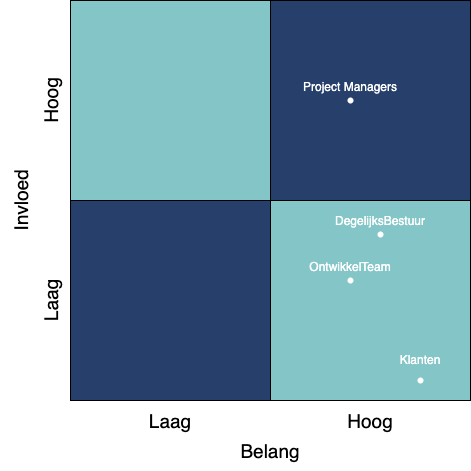
\includegraphics[width=10cm]{gfx/stakeholderanalyse}
    \caption{StakeHolders Analyse}
    \label{fig:StakeholderAnalyse}
\end{figure}
Zoals te zien is in figuur~\ref{fig:StakeholderAnalyse} zijn de projectmanager, het ontwikkelteam en de klanten het meest gebaad bij een nieuwe module voor de analyse van kwetsbaarheden.
Echter zijn de klanten niet tot bijna niet betrokken bij de ontwikkeling van de module maar hebben er indirect wel belang bij omdat de software die voor hen ontwikkeld wordt veiliger wordt door het voeren van een geautomatiseerde analyse.
Door deze analyse worden alleen de requirements meegnomen die intern zijn opgenomen.


\section{Gewenste situatie}\label{sec:gewenste-situatie}
Een situatie waar EagleScience naar toe wil is dat er periodiek of door middel van een trigger \footnote{Er kan bijvoorbeeld gedacht worden aan een commit op een branch zodat niet iedere dag een update wordt gedaan op De acceptence branche is een goed voorbeeld hiervoor} wordt onderzocht of er in de huidige dependency tree bibliotheken zitten die mogelijk kwetsbaarheden bevatten. Deze kennis dient gedeelt te worden door middel van een module in de portal die al reeds gebruikt wordt door EagleScience. Door de resultaten weer te geven in de portal ontstaat er een beter inzicht in welke bibliotheken we gebruiken en welke er potentieel kwetsbaarheden bevatten. Wat op zijn beurt weer voor veiligere applicaties kan zorgen. Ook voor de applicaties waar niet meer actief op ontwikkeld wordt. \footnote{Het is natuurlijk wel zo dat er een afhankelijk onstaat van externe bronnen die bekend moeten maken dat er een kwetsbaarheid is.}

\section{Requirements}\label{sec:requirements}
Naast het analyseren van de betrokkenheid en belang van de stakeholders is er ook gevraagd welke requirements ze terug wilden zien in de applicatie en welke prioriteit er aan gesteld werd.

Requirements kunnen worden opgedeeld in twee categoriën: "Functionele requirements" en niet-functionele requirements.

\subsection{niet functionele requirements}\label{subsec:niet-functionele-requirements}
Requirements voor de module die niet direct met de functionaliteit te maken hebben maar meer over omgevingen en dergelijke gaan.
\begin{itemize}
    \item Operationele requirements
        \begin{itemize}
            \item De methode moet zonder veel aanpassingen passen in de huidige werkstroom voor het ontwikkelen van software.
        \end{itemize}
    \item Omgeving requirements
        \begin{itemize}
            \item De module dient te worden ontwikkeld in Angular en Play(Scala), overeenkomstig met bestaande portal.
            \item De module dient gescheiden componenten te bevatten: Frontend(Angular), Backend(Play, Scala), API\@.
            \item De module dient in het Azure cluster te kunnen draaien binnen het huidige portal project.
        \end{itemize}
    \item Performance requirements
        \begin{itemize}
            \item De module moet op een zo efficient mogelijke manier een raport genereren.
            \item De module mag geen invloed hebben op de performance van de buildstraat.
        \end{itemize}
    \item security requirements
        \begin{itemize}
            \item Er dienen geen persoonsgegevens opgeslagen te worden die niet nodig zijn voor het functioneren van de module.
            \item Source code dient minimaal 70\% test coverage te hebben.
        \end{itemize}
\end{itemize}

\subsection{functionele requirements}\label{subsec:functionele-requirements}
\begin{itemize}
    \item De module dient eenvoudig gebruikt te kunnen worden in de huidige CI/CD pipeline voor bestaande en nieuwe projecten.
    \item De module dient ondersteuning te bieden voor meerdere omgevingen (OTAP)
    \item De module dient met een instelbaar interval een analyse uit te voeren op bestaande projecten.
    \item De module moet op project en omgevings niveau te rapporteren over bekende kwetsbaarheden.
    \item De module dient kwetsbaarheden op minimaal drie niveau's in te schalen(Kritish, gemiddeld en laag)
    \item De module dient ondersteuning te bieden voor het instellen van quality gates over meldingen die het vind op ieder niveau, per project, per omgeving.
\end{itemize}


\section{User stories}\label{sec:user-stories}
Naast de requirements uit de vorige sectie zijn er de volgende userstories opgetekend welke aangeven dat als deze geimplementeerd worden de module bruikbaar is voor de verschillende belanghebbenden. De userstories zijn onderverdeeld middels het MoSCoW principe.

\textbf{Must Have}
\begin{itemize}
    \item Als \textit{gebruiker} wil ik dat de SOUP-module in de portal te vinden is zodat alle tools die gebruikt worden binnen Eaglescience op een enkele plek te vinden zijn.
    \item Als \textit{gebruiker} wil ik een overzicht per project kunnen zien met daarin de gebruikte bibliotheken zodat ik inzage heb ik wat er gebruikt wordt voor ontwikkeling.
    \item Als \textit{gebruiker} wil ik een overzicht per project zien welke kwetsbaarheden er zich in bibliotheken bevinden, zodat ik actie kan ondernemen om de software nog veiliger te maken.
    \item Als \textit{gebruiker} wil ik in kunnen loggen met mijn LDAP account zodat ik niet nog een keer een username/wachtwoord combinatie hoe te leren.
    \item Als \textit{gebruiker} wil ik een project kunnen toevoegen zodat ik ook van dat project de kwetsbaarheden in kan zien en deze software ook veilger wordt.
    \item Als \textit{Module} wil ik een update krijgen van de laatste build met specifiek de laatste kwetsbaarheden, zodat ik deze kan weergeven in de portal.
    \item Als \textit{module} wil ik
    \item Als \textit{gebruiker} wil ik dat periodiek automatisch een check analyse wordt uitgevoerd zodat ik er zelf niet naar om hoef te kijken.
    \item Als \textit{gebruiker} wil ik zelf een analyse kunnen starten voor een project zodat ik een up-to-date versie heb van de resultaten.
    \item Als \textit{Project manager} wil ik projecten kunnen toevoegen aan de module, zodat ook deze mee genomen worden in de automatische analyse.
    \item Als \textit{Project manager} wil ik ontwikkelaars kunnen toevoegen aan een project zodat deze ook inzicht krijgen in de huidige stand van zaken.
    \item Als \textit{Project manager} wil ik een notificatie( via mail/rocketchat) ontvangen als er een kritieke kwetsbaarheid gevonden is.
\end{itemize}

\textbf{Should Have}
\begin{itemize}
    \item Moeten nog voorkomen uit de prioriteit analyse
\end{itemize}

\textbf{Could Have}
\begin{itemize}
    \item
\end{itemize}

\textbf{Won't Have}
\begin{itemize}
    \item Moeten nog voorkomen uit de prioriteit analyse
\end{itemize}
De Won't haves staan hierbij genoemd als leidraad voor eventueel updates in de toekomst.
Als blijkt dat er tussen de won'ts toch low hanging fruit blijkt te hangen kunnen deze meegenomen worden in de sprints.
De requirements worden als epics in een JIRA-omgeving gezet om vervolgens een planning te kunnen maken.

%    %TODO: Kijken of deze appendix nog relevant is, zo ja vertalen

\chapter{OWASP top 10}\label{ch:owasp-top-10}
%TODO: Uitwijden over wat de owasp is.
\section{Wat is de OWASP}
Het Open Web Application Security Project® (OWASP) is een stichting zonder winstoogmerk die zich inzet voor het verbeteren van de beveiliging van software. Door middel van door de gemeenschap geleide open-source softwareprojecten, honderden lokale afdelingen over de hele wereld, tienduizenden leden en toonaangevende onderwijs- en trainingsconferenties, is de OWASP Foundation de bron voor ontwikkelaars en technologen om het web te beveiligen.

Hulpmiddelen en bronnen
Gemeenschap en netwerken
Onderwijs en opleiding

Al bijna twintig jaar ondersteunen bedrijven, stichtingen, ontwikkelaars en vrijwilligers de OWASP Foundation en haar werk. Doneer, word lid of word vandaag nog zakelijk lid.

\section{OWASP top 10}\label{sec:owasp-top-10}
De OWASP top 10 wordt iedere 5 jaar uitgebracht om aan te geven wat de belangrijkste punten van aandacht zijn op het gebied van het veilig ontwikkelen van software. Met als doel om awareness te generen en zo software nog veiliger te maken. Hieronder staat een vrij vertaalde versie die op de website te vinden is. Zoals te zien is in figuur~\ref{fig:OWASPTop10Shifts} veranderd de focus iedere keer wat inhoud dat er werk gedaan wordt maar er nog steeds werk moet worden verricht.
\begin{figure}[bth]
    \myfloatalign
    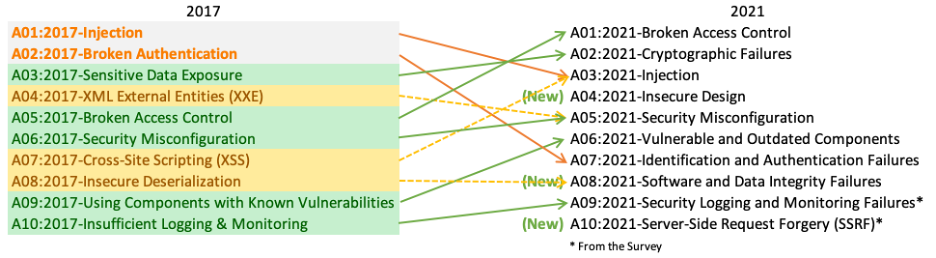
\includegraphics[width=10cm]{gfx/OWASPTop10 2017 to 2021}
    \caption{Verschuivingen OWASP Top 10 van 2017 naar 2021}
    \label{fig:OWASPTop10Shifts}
\end{figure}
\subsection{methode}
Om de top-10 samen te stellen wordt er gekeken naar de kwetsbaarheden gemeld in een CVE database. Waarbij er een gemiddelde wordt genomen van de exploit en impact score

In 2017, we selected categories by incidence rate to determine likelihood, then ranked them by team discussion based on decades of experience for Exploitability, Detectability (also likelihood), and Technical Impact. For 2021, we want to use data for Exploitability and (Technical) Impact if possible.

We downloaded OWASP Dependency Check and extracted the CVSS Exploit, and Impact scores grouped by related CWEs. It took a fair bit of research and effort as all the CVEs have CVSSv2 scores, but there are flaws in CVSSv2 that CVSSv3 should address. After a certain point in time, all CVEs are assigned a CVSSv3 score as well. Additionally, the scoring ranges and formulas were updated between CVSSv2 and CVSSv3.

In CVSSv2, both Exploit and (Technical) Impact could be up to 10.0, but the formula would knock them down to 60% for Exploit and 40% for Impact. In CVSSv3, the theoretical max was limited to 6.0 for Exploit and 4.0 for Impact. With the weighting considered, the Impact scoring shifted higher, almost a point and a half on average in CVSSv3, and exploitability moved nearly half a point lower on average.

There are 125k records of a CVE mapped to a CWE in the National Vulnerability Database (NVD) data extracted from OWASP Dependency Check, and there are 241 unique CWEs mapped to a CVE. 62k CWE maps have a CVSSv3 score, which is approximately half of the population in the data set.

For the Top Ten 2021, we calculated average exploit and impact scores in the following manner. We grouped all the CVEs with CVSS scores by CWE and weighted both exploit and impact scored by the percentage of the population that had CVSSv3 + the remaining population of CVSSv2 scores to get an overall average. We mapped these averages to the CWEs in the dataset to use as Exploit and (Technical) Impact scoring for the other half of the risk equation.
\subsection{Top 10}\label{subsec:top-10}
% TODO: door Google Translate halen
\begin{itemize}
    \item \textbf{A01:2021-Broken Access Control} moves up from the fifth position to the category with the most serious web application security risk; the contributed data indicates that on average, 3.81\% of applications tested had one or more Common Weakness Enumerations (CWEs) with more than 318k occurrences of CWEs in this risk category. The 34 CWEs mapped to Broken Access Control had more occurrences in applications than any other category.
    \item \textbf{A02:2021-Cryptographic Failures} shifts up one position to #2, previously known as A3:2017-Sensitive Data Exposure, which was broad symptom rather than a root cause. The renewed name focuses on failures related to cryptography as it has been implicitly before. This category often leads to sensitive data exposure or system compromise.

    \item \textbf{A03:2021-Injection} slides down to the third position. 94\% of the applications were tested for some form of injection with a max incidence rate of 19\%, an average incidence rate of 3.37\%, and the 33 CWEs mapped into this category have the second most occurrences in applications with 274k occurrences. Cross-site Scripting is now part of this category in this edition.

    \item \textbf{A04:2021-Insecure Design} is a new category for 2021, with a focus on risks related to design flaws. If we genuinely want to "move left" as an industry, we need more threat modeling, secure design patterns and principles, and reference architectures. An insecure design cannot be fixed by a perfect implementation as by definition, needed security controls were never created to defend against specific attacks.

    \item \textbf{A05:2021-Security Misconfiguration} moves up from #6 in the previous edition; 90\% of applications were tested for some form of misconfiguration, with an average incidence rate of 4.5\%, and over 208k occurrences of CWEs mapped to this risk category. With more shifts into highly configurable software, it's not surprising to see this category move up. The former category for A4:2017-XML External Entities (XXE) is now part of this risk category.

    \item \textbf{A06:2021-Vulnerable and Outdated Components} was previously titled Using Components with Known Vulnerabilities and is #2 in the Top 10 community survey, but also had enough data to make the Top 10 via data analysis. This category moves up from #9 in 2017 and is a known issue that we struggle to test and assess risk. It is the only category not to have any Common Vulnerability and Exposures (CVEs) mapped to the included CWEs, so a default exploit and impact weights of 5.0 are factored into their scores.

    \item \textbf{A07:2021-Identification and Authentication Failures} was previously Broken Authentication and is sliding down from the second position, and now includes CWEs that are more related to identification failures. This category is still an integral part of the Top 10, but the increased availability of standardized frameworks seems to be helping.

    \item \textbf{A08:2021-Software and Data Integrity Failures} is a new category for 2021, focusing on making assumptions related to software updates, critical data, and CI/CD pipelines without verifying integrity. One of the highest weighted impacts from Common Vulnerability and Exposures/Common Vulnerability Scoring System (CVE/CVSS) data mapped to the 10 CWEs in this category. A8:2017-Insecure Deserialization is now a part of this larger category.

    \item \textbf{A09:2021-Security Logging and Monitoring Failures} was previously A10:2017-Insufficient Logging & Monitoring and is added from the Top 10 community survey (#3), moving up from #10 previously. This category is expanded to include more types of failures, is challenging to test for, and isn't well represented in the CVE/CVSS data. However, failures in this category can directly impact visibility, incident alerting, and forensics.

    \item \textbf{A10:2021-Server-Side Request Forgery} is added from the Top 10 community survey (#1). The data shows a relatively low incidence rate with above average testing coverage, along with above-average ratings for Exploit and Impact potential. This category represents the scenario where the security community members are telling us this is important, even though it's not illustrated in the data at this time

\end{itemize}

%    % Appendix X

\chapter{Voortgang Module [Beter naam verzinnen]}

%TODO: MarginPARS zetten
%----------------------------------------------------------------------------------------
\section{Sprint 0}
\lipsum[01]
\subsection{Refinement}
\lipsum[01]
\subsection{Sprint verslag}
\lipsum[01]
\subsection{Retrosepctive}
\lipsum[01]

\section{Sprint 0}
\lipsum[01]
\subsection{Refinement}
\lipsum[01]
\subsection{Sprint verslag}
\lipsum[01]
\subsection{Retrosepctive}

%    \usepackage{lipsum}% Appendix X

\chapter{BegrippenLijst}\label{ch:begrippenlijst}


%----------------------------------------------------------------------------------------

% Content begins here

Goede manier vinden van onderscheiden zonder gebruik van secties....

\section*{Nog op alphabetische volgorde zetten!!!!!!}\label{sec:nog-op-alphabetische-volgorde-zetten!!!!!!}

\section{Docker}
\section{Kubernetes}
\section{Publish–subscribe pattern}
\lipsum[01]
\section{SOUP:}\label{sec:soup:} Software Of Unkown Provinence/Pedigree. is ook behandeld in de sectie~\ref{sec:dependency-trees?} in het kort is dit een weergave van dependencies en hun dependencies deze kan worden weergeven worden in een boom structuur.
\smallskip

\section{Dev-Stack:}\label{sec:dev-stack:} De ontwikkelomgeving die gebruikt wordt door een bedrijf. Dit is meestal een opsomming van gebruikte technologiën zoals Programeer talen, frameworks, en buildtools. Vaak worden ook andere tools genoemd zoald IDE's en andere Editors.
\smallskip

\section{Code smell:}\label{sec:code-smell:} De ontwikkelomgeving die gebruikt wordt door een bedrijf. Dit is meestal een opsomming van gebruikte technologiën zoals Programeer talen, frameworks, en buildtools. Vaak worden ook andere tools genoemd zoald IDE's en andere Editors.
\smallskip

\section{Linting:}\label{sec:linting:} De ontwikkelomgeving die gebruikt wordt door een bedrijf. Dit is meestal een opsomming van gebruikte technologiën zoals Programeer talen, frameworks, en buildtools. Vaak worden ook andere tools genoemd zoald IDE's en andere Editors.
\smallskip




\section{Dependency tree:}\label{sec:dependency-tree:} is ook behandeld in de sectie~\ref{sec:dependency-trees?} in het kort is dit een weergave van dependencies en hun dependencies deze kan worden weergeven worden in een boom structuur.
\smallskip

\section{Pure functie:}\label{sec:pure-functie:}
Een Pure functie is een functie die alleen een output genereerd op basis van een input dus als de functie \( y = x+1\) is dan geeft de functie bij een input van 2 dus 3 terug.
Een pure functie heeft dus geen side-effects die iets anders doen dan een output genereren op basis van de input.
Een applicatie bouwen met alleen maar pure functies is niet mogelijk gezien er nooit een I/O plaats kan vinden.
Deze I/O wordt dan ook meestal door een schil geregeld als in de volgende listing is te zien:
Zie \autoref{lst:pf} hieronder voor een voorbeeld.

%float=b,language=Scala,frame=tb, << Settings die eerst voor caption stonden
\begin{lstlisting}[caption={Pure functie met IO},label=lst:pf]


def abs(n:Int):Int =
  if(n<0) -n
  else n

def formatabs(x:Int): String = {
  val msg = "The absolute value of %d is %d"
  msg.format(x,abs(x))
}

//Unit is het Scala equivalent van Void in Java.
def main(args: Array[String]):Unit = {
  println(formatabs(-42)
}
\end{lstlisting}

Zoals te zien is de abs functie en pure functie gezien deze een input(Int) verwacht en alleen een output(Int) terug geeft.
Ook de format Abs is een pure functie er gaan twee input variabelen in en er komt altijd een String als output uit.
De waarde van de string is altijd hetzelfde bij dezelfde inputs.
De main functie is geen pure functie dit omdat er geen input en geen output is gedefineerd.
Echter, ontstaat er wel een output gezien er iets op de console wordt geprint door de println(formatabs(-42)) functie.
\smallskip

\section{JVM:}\label{sec:jvm:}
De JVM ook wel Java Virtual Machine is de runtime omgeving voor java applicaties.
Het voordeel is dat een JVM de runtime abstraheert van de os waardoor de applicaties geschreven in Java of een Java afgeleide taal kan worden uitgevoerd op verschillende bestuuringssystemen.
Dit wordt gedaan door middel van een compilatie van (Java)Sourcecode naar bytecode wat door de JVM wordt gecompileerd door het JIT (Just in Time) principe.
Dit komt de portabiliteit ten goede omdat er maar een enkele keer code geschreven hoef te worden wat zowel op mac, windows als linux hetzelfde gedraagt.
De JVM bied ondersteuning voor verschillende talen naast Java namelijk: Scala, Groovy en Kotlin.
\smallskip

\section{Time-to-market:}\label{sec:time-to-market:}
De marktintroductietijd is de tijdsduur benodigd om een product te ontwerpen totdat het op de markt verschijnt.
De benodigde tijd om een product op de markt te brengen is zeer belangrijk in industrieën waar de levensduur van een product kort is.
Bij een korte productlevenscyclus is het belangrijk, om winst te kunnen maken, om als eerste met het product op de markt te verschijnen.
\smallskip

\section{MoSCoW-methode:}\label{sec:moscow-methode:}
De MoSCoW-methode is een manier van prioriteiten stellen in onder meer de software-engineering.
De eisen aan het resultaat van een project worden ermee ingedeeld.
Het is een afkorting, waarvan de letters staan voor:

\textit{M} - must haves: deze eisen (requirements) moeten in het eindresultaat terugkomen, zonder deze eisen is het product niet bruikbaar;

\textit{S} - should haves: deze eisen zijn zeer gewenst, maar zonder is het product wel bruikbaar;

\textit{C} - could haves: deze eisen zullen alleen aan bod komen als er tijd genoeg is;

\textit{W} - won't haves: deze eisen zullen in dit project niet aan bod komen, maar kunnen in de toekomst bij een vervolgproject, interessant zijn.
De o's in de afkorting hebben geen betekenis
\smallskip

%    \chapter{TypeSetting Testst}\label{ch:typesetting-testst}

\section{Component diagram}


\section{Sequence diagram test}


Een aantal secties met tests om een bepaalde zaak uit te testen in \LaTeX
\section{mindmap test}\label{sec:mindmap-test}
Kijken of dit nog waardevol is:

\begin{tikzpicture}[grow cyclic, text width=2.7cm, align=flush center,
  level 1/.style={level distance=5cm,sibling angle=90},
  level 2/.style={level distance=3cm,sibling angle=45}]

  \node{ShareLaTeX Tutorial Videos}
  child { node {Beginners Series}
  child { node {First Document}}
  child { node {Sections and Paragraphs}}
  child { node {Mathematics}}
  child { node {Images}}
  child { node {bibliography}}
  child { node {Tables and Matrices}}
  child { node {Longer Documents}}
  }
  child { node {Thesis Series}
  child { node {Basic Structure}}
  child { node {Page Layout}}
  child { node {Figures, Subfigures and Tables}}
  child { node {Biblatex}}
  child { node {Title Page}}
  }
  child { node {Beamer Series}
  child { node {Getting Started}}
  child { node {Text, Pictures and Tables}}
  child { node {Blocks, Code and Hyperlinks}}
  child { node {Overlay Specifications}}
  child { node {Themes and Handouts}}
  }
  child { node {TikZ Series}
  child { node {Basic Drawing}}
  child { node {Geogebra}}
  child { node {Flow Charts}}
  child { node {Circuit Diagrams}}
  child { node {Mind Maps}}
  };
\end{tikzpicture}


\section{GANT CHART test}\label{sec:gant-chart-test}
\begin{figure}
  \begin{ganttchart}[hgrid=true,
  vgrid={*2{red}, *1{green}, *{10}{blue, dashed}}, x unit=1.2cm, y unit title=.6cm, y unit chart=.6cm]{1}{11}
  \gantttitle{2021 sprints}{11}\\
  \gantttitlelist{1,...,11}{1} \\
  \ganttgroup{Ontwerp}{1}{4}\\
  \ganttbar{interviews}{1}{2}\\
  \ganttlinkedbar{uitwerking interviews}{2}{3}\\
  \ganttlinkedbar{Design plan}{3}{4}\\
  \ganttmilestone{design approved}{4}\\

  \ganttgroup{Architectuur}{4}{5}\\
  \ganttbar{onderzoek }{4}{4}\\
  \ganttlinkedbar{ module integratie}{5}{5}\\
  \ganttmilestone{Architectuur approved}{5}\\
  \ganttgroup{Implementatie}{6}{11}\\
  \ganttmilestone{implementatie done}{11}\\

  \end{ganttchart}

  \begin{ganttchart}[hgrid=true,
  vgrid={*2{red}, *1{green}, *{10}{blue, dashed}}, x unit=2.4cm, y unit title=.6cm, y unit chart=.6cm]{1}{4}
  \gantttitle{2022 sprints}{4}\\
  \gantttitlelist{1,...,4}{1} \\
  \ganttgroup{Testing}{1}{4}\\
  \ganttmilestone{testing done approved}{4}\\

  \ganttgroup{Deployment}{2}{4}\\
  \ganttmilestone{Deployed}{4}\\
  \end{ganttchart}
  \caption{Planning}\label{fig:Planning}
\end{figure}


%----------------------------------------------------------------------------------------
%	POST-CONTENT THESIS PAGES
%----------------------------------------------------------------------------------------
%    \cleardoublepage% Bibliography

\chapter{Referencies}\label{ch:ref}

\cite{lamport94}



%\label{app:bibliography} % Reference the bibliography elsewhere with \autoref{app:bibliography}
%
%\manualmark % Work-around to have small caps also here in the headline
%\markboth{\spacedlowsmallcaps{\bibname}}{\spacedlowsmallcaps{\bibname}} % Work-around to have small caps also
%%\phantomsection
%\refstepcounter{dummy}
%
%\addtocontents{toc}{\protect\vspace{\beforebibskip}} % Place the bibliography slightly below the rest of the document content in the table of contents
%\addcontentsline{toc}{chapter}{\tocEntry{\bibname}}
%
%\printbibliography
 % Bibliography
%    \cleardoublepage% Declaration

\refstepcounter{dummy}
\pdfbookmark[0]{Declaration}{declaration} % Bookmark name visible in a PDF viewer

\chapter*{Declaration} % Declaration section text

\thispagestyle{empty}

Put your declaration here.
Diagrammen en tabellen zijn overgenomen van de bron echter is de layout/ kleurstelling aangepast aan de layout van dit document.
\bigskip
 
\noindent\textit{\myLocation, \myTime}

\smallskip

\begin{flushright}
\begin{tabular}{m{5cm}}
\\ \hline
\centering\myName \\
\end{tabular}
\end{flushright}
 % Declaration
%    \cleardoublepage% Colophon (a brief description of publication or production notes relevant to the edition)

\pagestyle{empty}

\hfill

\vfill

\pdfbookmark[0]{Colophon}{colophon}

\section*{Colophon}

This document was typeset using the typographical look-and-feel \texttt{classicthesis} developed by Andr\'e Miede. The style was inspired by Robert Bringhurst's seminal book on typography ``\emph{The Elements of Typographic Style}''. \texttt{classicthesis} is available for both \LaTeX\ and \mLyX: 

\begin{center}
\url{https://bitbucket.org/amiede/classicthesis/}
\end{center}

\noindent Happy users of \texttt{classicthesis} usually send a real postcard to the author, a collection of postcards received so far is featured here: 

\begin{center}
\url{http://postcards.miede.de/}
\end{center}
 
\bigskip

\noindent\finalVersionString % Colophon
%----------------------------------------------------------------------------------------
    \begin{thebibliography}{9}

        \bibitem{lamport94}\label{}
        Leslie Lamport,
        \textit{\LaTeX: a document preparation system},
        Addison Wesley, Massachusetts,
        2nd edition,
        1994.

        \bibitem{JanLeen2017}
        Jan Leen \& Jef Mertens,
        \textit{Praktijkgericht onderzoek in bedrijg},
        Tweede druk 2017,
        Uitgeverij coutinho, Bussum,

        \bibitem{wiki:SOUP}
        Wikipedia, auteur onbekend,
        \textit{https://en.wikipedia.org/wiki/Software\_of\_unknown\_pedigree}
        bezocht op 11-10-2021

        \bibitem{Kohnfelder2021}
        Loren Kohnfelder
        \textit{Designing Secure Software}
        november 2021

    \end{thebibliography}


\end{document}
